\documentclass[12pt]{article}
\usepackage[margin=1in] {geometry}                
\geometry{letterpaper}                   % ... or a4paper or a5paper or ... 
\pagestyle{plain}                           % Eliminates both the header and footer
\usepackage[parfill]{parskip}
\usepackage{graphicx}
\usepackage{amssymb}
\usepackage{epstopdf}
\DeclareGraphicsRule{.tif}{png}{.png}{`convert #1 `dirname #1`/`basename #1 .tif`.png}
\usepackage{amsmath, amsthm, amssymb}
\usepackage{array}
%\usepackage{pgfplots}
\usepackage{tikz}
\usepackage{tkz-euclide}
\usepackage{longtable}
\usepackage{caption}
\usepackage{subcaption}
\usepackage{verbatim}  %so that you can comment blocks of code
\usepackage{setspace}  %change the spacing
\usepackage[authoryear]{natbib}
\usepackage{bbm}
\usetikzlibrary{calc}
%\usepackage{csvsimple}
\usepackage[toc,page]{appendix}
\usepackage{hyperref}
\usepackage{cleveref}
\usepackage{rotating}
\usepackage{booktabs}
\usepackage{authblk}
\usepackage[bottom]{footmisc}
\usepackage{titling}
%% \newcommand{\KEYtitle}{Even Weights}
%\usepackage[nomarkers]{endfloat}
%\bibliography{library} 
%\renewcommand{\efloatseparator}{\mbox{}}
\usepackage{rotating}
\usepackage{pdflscape}
\usepackage[export]{adjustbox}
\usetikzlibrary{positioning}

%\usepackage{datetime}
%\newdateformat{monthyeardate}{\monthname[\THEMONTH]}


%\usepackage[dvipsnames]{xcolor}
%\usepackage{cite}
\onehalfspacing
\usepackage{natbib}  
\title{ Optimal Pricing and Informal Sharing: \\ Evidence from Piped Water in Manila }
\author{William Violette}
\affil{Brown University\thanks{ I am grateful to Andrew Foster, Matthew Turner, Jesse Shapiro, Daniel Bj\"{o}rkegren, and Bryce Steinberg for guidance and encouragement.  For helpful conversations, I am also grateful to John Friedman, Edward Glaeser, Emily Oster, Brian Knight, and Lint Barrage.  In Manila, thank you to the staff of my water company partner, government regulators at MWSS, as well as the USAID Be-Secure project for access to data and excellent conversations.  This work was supported through the Watson Institute for International and Public Affairs. } \\ [Job Market Paper: \href{https://drive.google.com/file/d/1dM41qZLZY3EPtUqHbca6MIS-nT77hv_-/view?usp=sharing}{\textcolor{blue}{Link to Current Version}}]}


\date{November, 2017}
\begin{document}

\maketitle
\begin{abstract}

%How should public utilities set fixed fees and marginal prices to provide access while covering costs?
%Why are there fixed vs. marginal?
%Public utilities recover fixed and marginal costs through a combination of fixed and marginal %prices.
%WHY CARE?! THE POOR!

	Public utilities subsidize fixed connection fees with high marginal prices to provide access especially for the poor, but this policy can have the opposite effect when many households share connections.  Using data on 1.5 million water connections in Manila, I establish that informal sharing networks provide 26\unskip\% 
	of total access.  I structurally estimate household water demand across three sources: purchasing directly from the provider, sharing with a neighbor's tap, or buying from a small-scale vendor.  The model predicts that low fixed fees and high marginal prices decrease access by weakening incentives to share water.  In contrast, the optimal pricing policy features high fixed fees and low marginal prices, increases shared connections, and ensures nearly universal access to piped water compared to current prices in Manila.  This policy improves welfare by up to 84\unskip\% of consumer surplus or 1.1\unskip\% of household income.

%	When households frequently share connections, this strategy may reduce access by weakening incentives to share.
%weaken incentives for households to extend water access to their neighbors through sharing 
%this strategy may have the opposite effect when connections are frequently shared between households.  
%	I analyze the welfare impacts of pricing for piped water in a context where households may choose to share their water connections with their neighbors.  
%	based on first-world experience


	%This policy improves welfare by up to 84\unskip\% of consumer surplus or 1.1\unskip\% of household income.

\end{abstract} 
{\bf JEL-Classification:} H23, L95, L98, O13, O17, O18 \\
\vspace{.1cm}
{\bf Keywords:} Water demand, non-linear pricing, informal sector, developing countries. 

\section{Introduction}
 
Despite large investments in piped water throughout the developing world, the share of urban households without piped water has remained stable at 5\% for middle income countries and at 20\% for low income countries for at least the past decade (World Bank [2015]).  Given health, time-savings, and other benefits from piped water, how can water utilities set prices in order to close gaps in access while still covering costs?\footnote{\cite{gamper2010impact,cutler2005role}, and \cite{galiani2005water} find health improvements in both developed and developing settings while \cite{devoto2012happiness} find time savings and other utility benefits.}  A popular approach particularly in developing cities is to subsidize upfront connection fees with high marginal prices to extend access especially for the poor.\footnote{\cite{mcintosh2003asian} and \cite{komives2006distributional} from the World Bank and Asian Development Bank argue for low connection fees.  Using a randomized controlled trial from Morocco, \cite{devoto2012happiness} confirm that modest assistance with connection fees can lead to increases in new water connections.}  In a similar spirit, over 70\% of developing cities increase marginal prices with monthly usage so that large users cross-subsidize access and usage for smaller, poorer users.\footnote{This strategy is also commonly referred to as ``Increasing Block Tariffs'' or  ``Convex Pricing'' (\cite{borenstein2012redistributional}). \cite{hoque2013state} and \cite{boland2000political} provide overviews of the use of increasing marginal prices in the water sector in developing countries.}  Recent empirical papers in South Africa and C{\^o}te d'Ivoire support this intuition, predicting gains in both access to piped water and total welfare from increasing marginal prices (\cite{szabo2015value,diakite2009proposal}). 






Conventional pricing policies often rely on the assumption that each water connection serves a single household; however, many households in developing cities share with neighbors instead of purchasing their own connections.  For example, 70\% of African cities report frequent water sharing (\cite{keener2010provision}) ranging from fetching from neighbors with hoses and buckets in Tangiers, Morocco (\cite{devoto2012happiness}) to drawing from single taps that each serve compounds in Kumasi, Ghana (\cite{whittington1992possible}).\footnote{\cite{nauges2006water} finds further evidence of widespread water sharing in Sri Lanka.}  In Manila, I establish that 23\% of households access water through a neighbor's connection by connecting plumbing directly to the meter (61\unskip\%), extending plastic pipes (25\unskip\%), or fetching water with containers (14\unskip\%).  While previous studies have focused on particular suburbs, this paper is the first to my knowledge to measure the role of water sharing in extending access across an urban population.

Water sharing has important implications for the welfare impacts of common pricing policies.  Increasing marginal prices weaken incentives for households to extend water access to their neighbors through sharing (\cite{whittington1992possible}).  Fixed fee subsidies may have limited impacts on water access when sharing households split connection fees with their neighbors.  Since low-income households are more likely to use water from their neighbors, increasing marginal prices and low fixed fees may combine to act as regressive taxes in the presence of sharing.  

%  Shared connections record high levels of monthly consumption, which can expose them to high prices when marginal prices increase with usage . 
This paper analyzes the welfare impacts of pricing policies in the presence of informal water sharing.  Welfare impacts depend not only on heterogeneity in demand for water across the population, but also on costs associated with forming and maintaining water sharing relationships.  To measure these features, I merge administrative data covering 1.5 million water connections in Manila from 2010 to 2015 with detailed survey data on the number of households and people using each water connection.  With comprehensive geographic coverage of half of Manila and a variety of price variation, these data allow for a rich characterization of water demand.  Additional variation in water source choices identify the relative fixed and marginal costs associated with sharing water with a neighbor.  I find that despite relatively high marginal costs of sharing, shared connections allow the city to save on installation and maintenance costs, providing an efficient means for extending piped water to low-demand households at low marginal prices.  At the same time, informal sharing networks act as resale markets for water, undermining the extent to which cities can redistribute surplus through increasing marginal prices.

To evaluate the impacts of different pricing policies, I build a model of household water demand that includes both initial source choices as well as monthly consumption choices.  This model expands on the demand estimation literature for public utilities that focuses almost exclusively on quantity choices (\cite{diakite2009proposal,mcrae2014infrastructure,olmstead2009reduced,szabo2015value}).  I specify a sequential game where households choose whether to connect individually, share with their neighbors, or purchase from a water vendor.  For sharing households, I develop a simple model of the water sharing contract that captures two key features of these relationships: (1) households face challenges in observing each other's demand and (2) households often split the monthly water bill evenly.  The model characterizes monthly consumption choices when households face non-linear budget constraints and imperfect control over their exact consumption levels.  This approach extends previous models of optimization over non-linear budget constraints by allowing households to anticipate unobserved shocks to their demand (\cite{moffitt1986econometrics,burtless1978effect}).

The estimation combines water source and consumption decisions to structurally recover preferences and unobserved costs of water sharing.  To include reduced-form approaches to identification within the context of a structural model, I divide the estimation into three steps.  The first step uses variation in the non-linear price schedule (both across and within households) to identify water demand for each household using monthly consumption data.  To measure the shadow costs of fetching water from a shared connection, the second step analyzes a quasi-experiment where households face leaks in their service pipes, forcing them to substitute to a neighbor's connection.  The model maps the extent to which these households are able to offset their consumption to a neighbor's connection into an estimate of the marginal costs of fetching water.  This exercise recovers sizable sharing costs on the order of 63.7\unskip\% of the average marginal water price.  This quasi-experimental approach builds on a descriptive literature pointing to potential costs of sharing water (\cite{whittington1992possible,nauges2006water}).  On top of an initial connection fee and monthly service fee, households may face unobserved fixed costs in owning a connection, which may include application costs, plumbing maintenance, as well as land-tenure issues in qualifying for a water connection.  The third step estimates these fixed costs by simulating the sequential game to match cross-sectional variation in water source choices.  This strategy provides a structural, revealed-preference approach to recovering unobserved fixed costs, complementing previous reduced-form evidence in \cite{devoto2012happiness}.

Combining the model and estimates, I simulate a series of counterfactual policies.  First, I consider a connection fee subsidy policy consistent with recommendations from the World Bank, NGOs, and other researchers to improve water access for the poor (\cite{komives2005water,wsup,jimenez2014factors,mcintosh2003asian}).  I discount the fixed fee by 12\% while increasing the tariff schedule proportionally to ensuring that the water provider exactly covers costs.  This policy reduces access by incentivizing households to substitute away from sharing arrangements toward both individual connections and water vendors (which mainly include deepwells and water refilling stations).  

Next, I compute an optimal tariff schedule to maximize consumer surplus while exactly covering production costs.  Compared to the current tariff, I find that a simple, two-part tariff characterized by a fixed fee and low, flat marginal price can produce gains on the order of 84\unskip\% of consumer surplus or 1.1\unskip\% of household income.  These gains are driven both by pricing closer to marginal cost as well as by increasing sharing, which reduces the number of connections to install and maintain.  Yet, since sharing involves costly redistribution of water, the optimal tariff subsidizes individual connections on the margin by pricing above marginal cost and setting the fixed fee below the cost of installing and maintaining each connection.

Finally, I compare the optimal tariff with a social tariff that maximizes consumer surplus only for the bottom 50\% of users and is intended to capture goals of ensuring minimum usage and access as well as income redistribution.  The social tariff features a much higher fixed fee and lower marginal price, does not improve access to piped water, and reallocates little consumer surplus to low-demand households at a large cost to average welfare.  By contrast, in a counterfactual world without sharing, the social tariff features a fixed fee subsidy and increasing marginal prices; it also increases access and efficiently redistributes consumer surplus to low users as compared the optimal tariff.  These results provide evidence that the presence of informal sharing networks constrains pricing policy as an effective tool for redistribution.

In focusing on water sharing behavior, this approach abstracts away from several features that may also affect optimal pricing policy.  First, I do not directly model environmental, health, or other externalities associated with piped water use.  From a policy perspective, water shortages may lead policymakers to promote conservation through higher marginal prices while positive health externalities may motivate further subsidizing piped water (\cite{timmins2002measuring}, \cite{galiani2005water}).\footnote{\cite{bennett2012does} shows that piped water can also lead to negative externalities through worse sanitation, possibly motivating higher prices for piped water.}  Second, I assume that government regulator is able to fully observe production costs for the water provider, eliminating scope for prices to correct for possible principal-agent frictions as characterized by \cite{laffont1993theory}.  Finally, the counterfactual exercises borrow the public-private partnership regulatory framework in Manila by assuming that revenue must fully cover production costs.  Additional data on the costs of raising public funds and risks of regulatory capture would allow for a more flexible analysis taking into account the possibility of public funding for water (\cite{laffont2005regulation}).  

% Despite the relevance of water sharing arrangements to pricing policy, previous studies have provided either a descriptive analysis of water sharing (\cite{whittington1992possible}) or 
% in fixed fee incentivizes households to substitute away from water sharing arrangements toward individual connections as well as  , it also increases the share of households using from a local 
%among low-demand households by as much as \input{tables/discount_low_welfare_change}\unskip\% of monthly income.  
%%%% WHAT IS ACCESS DUDE!!!!!!!

The next section describes the context of water provision in Manila.  Section~\ref{section:data} describes the data.  Section~\ref{section:patternsofwateruse} presents stylized facts about water usage in Manila.  Section~\ref{section:modelofhouseholdwateruse} introduces a model of household water usage and source choices.  The estimation is divided into three steps in Section~\ref{section:specificationandestimation}.  Section~\ref{section:preferenceestimation} uses monthly quantity choices and price variation to estimate preferences.  Section~\ref{section:hasslecostestimation} analyzes a quasi-experiment to recover an estimate of the marginal costs of sharing with a neighbor.  Given these estimates, Section~\ref{section:fixedcostestimation} recovers the relative fixed costs of owning a connection or using from a vendor.  Section~\ref{section:counterfactualexercises} uses these estimates to examine counterfactual pricing policies.  Section~\ref{section:conclusion} concludes.

%%  This strategy has counterintuitive effects in a context with widespread sharing by subsidizing costs for high

%%  Served by a large, government-regulated water monopoly, Manila provides an ideal setting since over 43\unskip\% of households share water connections.  Given many positive health exernalities from access to safe, reliable water (\cite{galiani2005water,gamper2010impact,kremer2011spring}), redesigning pricing regimes to boost access and usage especially among the poor can have significant welfare consequences.

%%  Over 70\% of developing cities have water pricing regimes characterized by high fixed connection fees and marginal prices that increase with monthly usage to cross-subsidize low-income users (\cite{hoque2013state}).  From a theoretical perspective, the optimal pricing strategy to maximize surplus especially for low-income households while covering costs of production depends on the frictions associated with sharing water.  These sharing frictions may include time costs fetching water from a neighbor as well as difficulties dividing the monthly water bill among sharing households.  If sharing frictions are large, policymakers may want to disincentivize sharing by implementing a low fixed fee and increasing the marginal price schedule.  On the other hand if sharing frictions are small, policymakers may instead use a high fixed fee and alongside a decreasing marginal price schedule in order to encourage sharing networks, set marginal prices closer to marginal costs, and minimize the number of connections that would need to be installed.  This paper provides empirical estimates of these sharing frictions in an effort to guide these pricing decisions.

%%  From a theoretical perspective, the impacts of this pricing regime depend on the frictions associated both with sharing water as well as connecting to the network.  These sharing frictions may include time costs fetching water from a neighbor as well as difficulties dividing the monthly water bill among sharing households.  If sharing frictions are high, policymakers may want to disincentivize sharing by implementing a low fixed fee and increasing marginal price schedule.  COME BACK TO THIS ISSUE: DO I WANT TO GET INTO OPTIMAL SO SOON!? NOT SURE....

%%  While low-cost sharing networks constrain the set of efficient pricing strategies available to the regulator, these networks ultimately improve welfare for low-income households by providing an additional mechanism for these households to access low-cost piped water.

%%  This paper contributes most directly to an expanding literature on estimating demand for public utilities in developing countries, including water in South Africa (\cite{szabo2015value}) and C{\^o}te d'Ivoire (\cite{diakite2009proposal}) and electricity in Colombia (\cite{mcrae2014infrastructure}).  Previous work has focused on how pricing affects monthly consumption decisions.  This paper extends these models by allowing households to also choose their initial water source.  By structurally modeling source choice, this paper also connects to a small reduced-form literature that emphasizes the importance of fixed costs associated with connecting to a piped water network (\cite{devoto2012happiness,jimenez2014factors,kayaga2007costs}).




\section{Water Provision in Manila}

In 1997, citing poor service quality and low coverage of the public water provider, the Philippines conducted the largest water privatization in the developing world.  Two private companies evenly divided the city into east and west zones as part of a public-private partnership.  Both companies invested heavily in infrastructure, which has resulted in near universal availability of piped water services for Manila.  A government regulator oversees these companies and implements rate-of-return regulation: water tariffs are revised periodically in order to ensure that providers recover all operating costs as well as earn a percentage return on any capital investments.  Rate-of-return regulation is common in developing countries since high costs of public funds as well as high risks of regulatory capture limit funding of utilities through government revenue (\cite{laffont2005regulation}).

This paper focuses on one of the providers which serves 1.5 million connections and around 5 million people.  Figure~\ref{figure:tariff} shows the regulated tariff in Manila.  The increasing marginal price is thought to cross-subsidize consumption among low-demand, poorer households through higher bills from large users.  The regulator assigns zero marginal price to the first 10 cubic meters of monthly usage, which is called the ``lifeline'' rate.  This policy is intended to provide a minimum level of consumption for all households.  This tariff may also perform efficient price discrimination if low-usage households are more price-sensitive.
\begin{figure}
\centering
\caption{Water Tariff in Manila}\label{figure:tariff}
\begin{center}
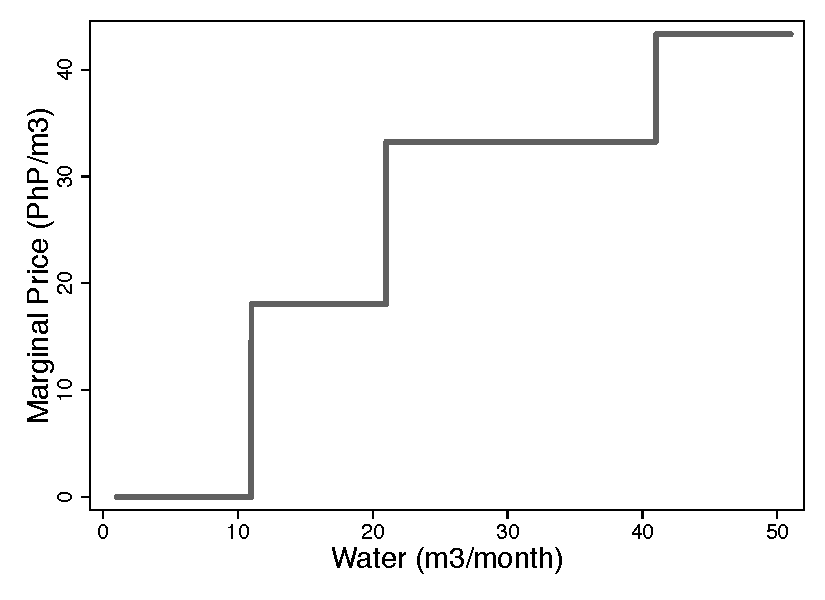
\includegraphics[scale=.7]{tables/tariff_structure.pdf}\\
\footnotesize{1 USD = 50 PhP}
\end{center}
\end{figure}
% detail more about how to get water, with the fixed fee and conne{}ction fee?!
On top of this tariff schedule, the regulator also charges a fixed fee independent of usage totaling 225 PhP/month.  This fee includes both the monthly service charge and the initial connection fee that I have put into monthly terms for the duration of the water connection.\footnote{Appendix~\ref{appendix:connectionfeeamortization} provides more details about how this monthly fee is calculated and amortized.}  The fixed fee allows the provider to recover any operating costs associated with serving the connection.  This form of increasing tariff and fixed fee combination is implemented in over 70\% of developing cities as well as over 50\% of developed cities (\cite{hoque2013state}).

Faced with this fixed fee as well as other costs associated with getting and maintaining a connection such as additional application costs or land tenure insecurity, I find that over 23\unskip\% of households use a neighbor's tap in Manila.  Sharing a connection with a neighbor mechanically increases the total monthly consumption recorded per connection, often doubling the marginal prices faced by these households compared to using a connection alone.  Although most households use piped water either through their own or neighboring connections, 6\unskip\% of households remain unconnected to the network and instead fetch water primarily from nearby deepwells while some use water refilling stations or other vendors.



\section{Data}\label{section:data}

%Monthly quantity choices across different households and at different prices reveal information about household demand.  Observing multiple quantities choices for the same household allows for a rich characterization of demand heterogeneity at the household-level.  
Evaluating different pricing policies requires measuring demand at the household level as well as costs associated with providing piped water.  For information about these attributes, I developed a partnership with one of the regulated, private providers in Manila who provided both billing records as well as information about the regulatory structure, pricing, and production costs.  Complete billing records for each water connection including the monthly meter reading, the total bill charged, and the precise location for each meter serve as the primary measure of quantity choices.  These data span 2010 to 2015, during which connections grew from 800,000 to 1.5 million water connections, generating nearly 100 million transaction records.  Connections are divided into residential (90\%), semi-business (4\%), commercial (5\%), and industrial (1\%).  This paper focuses on residential and semi-business connections.\footnote{Semi-business connections are largely composed of households that own small roadside stands.  These connections provide a useful source of price variation which is described in Appendix~\ref{appendix:ratechangeelasticity}.}  The monthly meter reading is used as the measure of consumption for each connection.  Meter readings are rounded to the nearest cubic meter, and I limit consideration to meter readings below 120 $\text{m}^{3}$ in order to exclude pipe leaks as well as meter reading errors (readings above 120 $\text{m}^{3}$ compose less than 0.5\% of the sample).

Since the object of interest for welfare is household-level demand, I merge the billing records to unique survey data recording information on households using each connection.  To evaluate the performance of the water provider, the regulator contracted with a local university to conduct the Public Assessment of Water Services (PAWS) in three waves from 2008 to 2012, surveying around 50,000 water connections.\footnote{Appendix~\ref{appendix:pawssampling} describes the sampling design and tests the extent to which it may be correlated with demographic characteristics.  This exercise finds relatively weak correlations in economic terms with key characteristics.}  I have collected unique identifiers for this survey, which allows responses to be linked to water connections.  The connection survey records the total number of households and people using each connection, providing the primary measure of sharing behavior.  The connection survey also includes basic demographics for the owner of the connection.  The demographics used in this paper are household size, dwelling type (whether apartment, duplex, or single house), number of employed household members, and whether the head of household is employed in a low-skill profession.
%consumption and water source choices at the household-level.  
%To examine both consumption decisions and water source choices at the household-level, I construct a dataset that merges (1) monthly water usage for around 50,000 connections, (2) demographics and water sharing measures for households using these connections, and (3) a cross-section of all households and their water source choices.  Put together, these data form a representative sample of households in half of Metro Manila.

A full analysis of water usage in Manila also requires describing households that choose to use water from local vendors.  For information on households that are using water from alternative sources, I turn to the 2010 Census of Population and Housing.  Households are defined as connected to the piped network if they report using a ``faucet community water system'' for their cooking, laundry, or bathing needs.\footnote{The census was designed largely for rural populations so it does not directly ask whether households are connected to a piped water network.}  Alternatively, I define households as using from a water vendor if they report any other category, which includes deep wells, peddlers, or other sources.  I then construct similar demographic measures to the connection survey using questions in the census and compare these measures across these data sources in Table~\ref{table:pawstocensus} of Appendix~\ref{appendix:pawstocensus}.  Households that own a connection in the connection survey are similar to households connected to the piped water network in the Census data.  To construct a profile of water source choices for the full population, I randomly sample from the pool of households using from vendors in 8 regions of the city so that the data form a representative sample when combined with households covered by the connection survey in each small area.\footnote{Regions are chosen to overlap with village administrative/political boundaries while ensuring that I am able to obtain a large enough sample of vendor households for each area to perform the counterfactual analysis in Section~\ref{section:fixedcostestimation}.}

For additional information on water sharing relationships between households, I fielded a small, non-representative survey of 600 households via mobile phone app.  This survey asks about issues associated with using different water sources, basic demographics, as well as how the bill and connection fee are paid for sharing households.  Appendix~\ref{appendix:pollfish} includes additional details on this survey and finds roughly similar measures between the connection survey and the mobile survey, suggesting that the mobile survey may provide a reasonable descriptive picture of sharing in Manila.

The water provider also maintains call records of all service complaints, which can be linked to individual connections.  This data is used to measure instances where households face unanticipated shocks to their water source as part of the identification strategy to estimate the hassle costs of sharing water.  Finally, the water provider tracks data on the marginal cost of pumping an additional cubic meter of water as well as the costs associated with installing new connections.  These data provide inputs into the provider's budget constraint, which are necessary for computing counterfactual pricing regimes.  Supplemental survey data from a subset of Manila include income measures that are used to impute income for the remainder of the sample across a variety of demographic variables and their interactions.


\section{Patterns of Water Use}\label{section:patternsofwateruse}

The welfare consequences of informal sharing networks depend on both the types of households that choose to share with neighbors as well as the costs of these networks.  To provide some descriptive evidence, Table~\ref{descriptives} merges the connection survey of water connections with billing records associated with each connection.  The columns group connections by the number of households they serve: one, two, or at least three.  

The first rows provide demographic information from the connection survey for households who own connections.  Smaller and younger households are more likely to share water with neighbors.  Because household size is a strong proxy for water demand, this finding suggests that sharing a connection is negatively correlated with household water demand.  Households with lower imputed income more commonly share water connections.  Sharing households are over twice as likely to reside in duplexes possibly because transporting water between neighbors requires less effort for duplex residents.

\begin{table}
\centering
\captionsetup{justification=centering}
\caption{ Water Connections  by Number of Households Served}\label{descriptives}
\begin{tabular}{l*{1}{ccc}}
%\hline
%\hline 
 &Serving One &Serving Two &Serving Three  \\
 &Household &Households &or More Households  \\
\hline

\textbf{Owner Demographics} &\multicolumn{3}{c}{ }\\
%\hline
Age (Head of HH) &       46.8  &       46.4  &       45.1   \\
HH Size &       5.32  &       4.68  &       4.49   \\
Total Empl. &       1.64  &       1.43  &       1.32   \\
Low-Skill Emp. (Head of HH) &         0.15 &          0.19 &         0.21  \\
Inc. (USD/Mo. Imputed) &        405  &        379  &        369   \\
Apartment &          0.24 &          0.13 &          0.13  \\
Single House &          0.62 &          0.52 &          0.38  \\
Duplex &          0.14  &          0.35 &          0.49  \\
 & &  & \\
\textbf{Connection Attributes} &\multicolumn{3}{c}{ }\\
%\hline
Water (m3/mo.) &      24.66  &      32.30  &      42.59   \\
Water Bill (USD/Mo) &      10.32  &      15.06  &      22.54   \\
Total People Served &       5.32  &       8.94  &      15.29   \\
Water per Person &       5.09  &       3.86  &       3.04   \\
 & &  &  \\
\textbf{Sample} &\multicolumn{3}{c}{ }\\
%\hline
Connected HHs &     42,798  &     16,930  &     19,896   \\
Share of Connected HHs &          0.54 &          0.21 &          0.25  \\
Months per Connection &         52  &         49  &         45   \\
%\hline
\hline
\end{tabular} \\
\footnotesize{The data include billing records merged with the connection survey. \\ Income is imputed using location, demographic variables, and their interactions.}
\end{table} 

Table~\ref{descriptives} also summarizes water use and sharing behavior for these connections, merging information from the connection survey with the billing records.  Larger numbers of households sharing a water connection are correlated with higher total water usage, but less water per person.\footnote{Total People Served by a connection includes both the owning household and any other households using a connection.}  This decline in usage per person may have many possible drivers: (1) sharing households face higher prices by locating at a higher point on the tariff schedule (Figure~\ref{figure:tariff}), (2) sharing households may face hassle costs in fetching water from neighboring taps, (3) these price effects may incentivize low-demand households to select into sharing relationships, consistent with the demographic patterns, and (4) low-demand households may have idiosyncratic preferences for sharing relationships.  On average, monthly water bills (inclusive of service fees) take up around 3\unskip\% of household income, which does not include other unobserved costs in accessing water.  These findings suggest that policies which affect sharing choices can have significant welfare consequences.  

%Also, the mobile survey indicates that only around 30\% of sharing households would substitute to toward a neighbor's connection if they no longer had access to their primary water source.  For this reason, I treat connections reported to serve more than three households as only serving three households.  
Table~\ref{descriptives} also computes the total number of households using from each source.  I assume that households sharing with one or two other households are uniquely linked to one connection so that the population of households connected to the network can be computed by summing the number of households served by each connection.  This assumption is consistent with the presence of fixed costs in setting up a connection or a sharing relationship.  To the extent that households are drawing water from multiple connections, this assumption may lead to an overestimation of the population engaged in sharing relationships.  Under this assumption, I find that 54\unskip\% of connected households receive their water from an individual connection, 21\unskip\% are involved in a sharing relationship with a single neighbor, and 25\unskip\% are in a sharing relationship with 2 or more other households.  These proportions do not take into consideration households that are using from water vendors, which are discussed in more detail below.  Each water connection contributes over six years of billing records on average.

Since the connection survey only includes households connected to piped water, I use census data to learn about households using from water vendors.  6\unskip\% of the population report using vendors, which is composed of 76\unskip\% of households using from a ``deep well'' and 17\unskip\% using from a ``peddler'' while the remaining fall into an ``other'' category.  Anecdotal evidence suggests that groundwater from wells often has very low quality.  Appendix Table~\ref{table:pawstocensus} compares means of demographic variables between connection owners from the connection survey and all households from the census.  Demographic variables are similar between connection owners in the connection survey and the census data.  Households using from vendors have lower imputed incomes, greater probability of low-skill employment, and slightly fewer members than own-use households.  Across most dimensions, households using from vendors more closely resemble households that share with their neighbors as opposed to households that use their connections individually.

%  While demographics are broadly similar between the first and second columns, any differences are likely driven by two factors.  First, connection owners may have different demographic characteristics than households using from a neighbor's tap.  This explanation is consistent with larger household sizes and lower rates of low skilled employment among connection owners in the first column relative to connection owners and other users captured in the second column.  Second, demographic measures may not be exactly comparable across these surveys.  Consistent with this theory, easily measured demographics like age of household head, household size, and total household members employed are very similar across the first and second columns; however, more subjective measures such as level of skill in employment and type of dwelling exhibit greater variation across data sources.  For this reason, the imputation strategy used in Section~\ref{section:fixedcostestimation} also relies on local geographic measures alongside these demographic measures.










\section{A Model of Household Water Use}\label{section:modelofhouseholdwateruse}
% Given that households derive utility from a water source through a stream of water use, 
% Taking these observed choices as inputs, this model is designed to recover both preference parameters for water as well as the shadow costs of using different water sources.  

This section presents a stylized model of water source choice and monthly quantity decisions at the household level.  This model allows for an analysis of the impacts of pricing policies on both source and quantity margins, which are often equally relevant to policymakers (\cite{mcintosh2003asian,komives2005water}).  Using both margins also enables the estimation to include cross-sectional variation in sources alongside time-series variation in quantities to recover a broad set of demand and cost parameters.

Let the city of Manila be partitioned into neighborhoods, where each neighborhood is defined by a set of households that are physically close enough to share water connections with each other.  In the context of Manila, these neighborhoods are often characterized by dense clusters of houses or duplexes.  This partition embeds the assumption that neighborhoods are mutually exclusive so that a household located in one neighborhood cannot share water with households in a nearby neighborhood.  Restricting the choice set in this way may tend to overestimate the costs that households face in finding a sharing partner.\footnote{This limitation is discussed in more detail in Section~\ref{section:fixedcostestimation}}

In the first period, each household makes a one-time decision about their water source between purchasing a connection, using a neighbor's connection, or buying from a local water vendor.  These decisions result in a set of water connections for each neighborhood ranging from an empty set if all households use from a vendor to equaling the size of the neighborhood if each household uses an individual connection.  If households choose to connect to the network, each connection, $C$, serves a set of households given by $S$, which depends on which households have decided to share the water connection.  Also, let the index $C$ indicate connection-level attributes, summing over all households using connection $C$.  This model does not allow for households to choose different water sources over time, which is consistent with large fixed costs involved in initially purchasing a connection or establishing a sharing relationship.  At the same time, some households may exogenously lose access to their water source, forcing these households to substitute toward other sources as detailed in Section~\ref{section:hasslemodel}.

Conditional on their water source choice, households then choose how much water to use each month.  Since water sources provide utility through monthly consumption, this section describes the decision process in reverse order, first characterizing monthly water consumption choices (taking the initial source choice as given) and second, describing the water source choice (according to the expected utilities from using each source).

\subsection{Consumption Choices for Households Using Piped Water}\label{section:consumptionchoice}
% The goal is to take water consumption data and map it into preferences...
% Water consumption data for each connection aggregates the monthly consumption for all households as well as individuals within these households. 
% Modeling this behavior is not only useful for accurately characterizing demand, but may also play an important role in measuring the potential welfare losses from these non-linear pricing schedules.  
%(CITE JAYACHANDRAN AND JACK)

This section details how households choose their monthly quantities of consumption holding their water source fixed.  For households using piped water, this consumption choice is complicated by four features:  (1) households may have difficulty targeting their exact monthly consumption levels; (2) increasing marginal prices in the water tariff result in non-linear budget constraints; (3) households that share a connection need to determine how to divide the monthly water bill; and (4) households fetching from a neighbor may face additional hassle costs in transporting water.  Since the data record monthly consumption for each connection, this model first introduces individual household demand before aggregating household demand at the connection-level for estimation.

Households that use piped water face the difficult task of coordinating water consumption among all household members.  For example, consider a household head trying to manage water consumption across all of their household members each month.  This task would involve monitoring the meter located outside of their dwelling and observing water use among all members.\footnote{Given that many developing countries feature steeply increasing prices with monthly usage, these coordination challenges may magnify any distortions caused by non-linear pricing.}  Mobile survey data indicate that 43\unskip\% of surveyed household members do not recall how much they paid for water in the last month while 64\unskip\% do not recall the amount that their household consumed in the previous month.  

As a simple way to capture this coordination task, the model assumes that each household $i$ sets a goal for water use each month, $w_i$, knowing that idiosyncratic factors, $\epsilon_i$, may increase or decrease the realized amount of usage.  Consumption shocks, $\epsilon_i$, are assumed to be unobserved to the household and independent across time, bringing the total realized water consumption each month to, $W_i=w_i+\epsilon_i$.  Household utility over water, $W_i$ and a numeraire good, $x_i$ is assumed to take the following shape:
\begin{align}\label{equation:umaxfirst}
\begin{split}
U(x_i,W_i) &=  x_i + W_i - \frac{1}{2\alpha_i } ( W_i - \Gamma_i + \alpha_i )^2  \\
W_i &= w_i + \epsilon_i \\
\epsilon_i &\sim \mathcal{N}(0,\Sigma_{\epsilon})
\end{split}
\end{align}
Following from quasi-linear preferences, this quadratic form for utility eliminates income effects and includes a natural satiation point for water consumption, capturing the tendency of households to target specific consumption levels despite low or zero marginal prices as in Figure~\ref{figure:consumptionhistogram}.  Household preferences for water are characterized by $\Gamma_i$, which can be interpreted as a fixed preference for water each month and $\alpha_i$, which captures the extent to which households are price sensitive.  These terms have clearer interpretations in the demand function below.  The exogenous shock to consumption, $\epsilon_i$, is assumed to be drawn from a multivariate normal distribution, $\Sigma_{\epsilon}$ with zero mean, variance terms, $\sigma_{\epsilon}^2$, and allowing for correlation with neighboring households, ${\rho}^{\epsilon}_{i,j}$.  Although households cannot anticipate the exact realization of $\epsilon_i$, they are assumed to understand the distribution of possible shocks, allowing them to maximize expected utility.
\subsubsection{Determining the Budget Constraint}
The household problem is additionally complicated by the presence of non-linear price schedules for water.  Figure~\ref{figure:tariff} provides the increasing tariff in Manila.  The non-linear price schedule produces kinks in household budget constraints leading to non-linear demand functions.  Let $P(W_C) = \{ p^{1},...,p^{K},\overline{W}^{0},...,\overline{W}^{K}\}$ describe tariff schedule as a function of total consumption for the water connection, $W_C = \sum_{i=1}^{S} W_i$.  The tariff includes $K$ segments where segment $k$ corresponds to price $p^{k}$ for water consumption between the consumption thresholds (or kink points), $\overline{W}^{k-1}$ and $\overline{W}^{k}$:
\begin{align*}
P(W_C)=&  
\begin{cases}
      p^{1} &\text{ if } W_C \in [\overline{W}^{0}(=0),\overline{W}^{1}], \\
      p^{2} &\text{ if } W_C \in [\overline{W}^{1},\overline{W}^{2}], \\
      ...   &\text{ ...}, \\
      p^{K} &\text{ if } W_C \in[\overline{W}^{K-1},\overline{W}^{K}(=\infty)]
    \end{cases}
\end{align*}
Given prices and household utility, the final ingredient for characterizing consumption choices is the budget constraint.  The budget constraint includes monthly household income, $Y_i$, and monthly fixed costs of using the water connection, $F_i$, which are assumed to capture three components: (1) monthly service fees, (2) initial connection fees amortized in monthly terms for the duration of the connection, and (3) unobserved, fixed hassle costs associated with setting up a connection, which are also amortized into monthly terms.  Data does not track household water source choices over time in a comprehensive way, which limits the extent to which the model can distinguish between one-time connection costs and monthly service/maintenance costs.  This limitation means that the model cannot address the optimal timing of fixed payments or capture any potential heterogeneity in monthly fixed costs.

Water sharing relationships impact monthly consumption choices through the budget constraint in three ways.\footnote{While the formation of these relationships is discussed in more detail in Section~\ref{section:watersourcechoice}, this section takes these sharing relationships as exogenously given.}  To develop notation for sharing, normalize $i=1$ to be the owner of the connection and define the total number of sharing households for a particular connection as $S$.

First, this model assumes that the monthly water bill is split evenly between all sharing households.  Descriptive evidence suggests that challenges observing and coordinating usage within members of a household also extend across households.  Among owners of the water connection responding to the mobile survey, 28\unskip\% report splitting the water bill evenly or alternating payment each month, 27\unskip\% charge sharing households a fixed amount each month regardless of their consumption, and 36\unskip\% charge other users a price according to their usage.\footnote{The remaining households report ``I don't know'' or ``other.''}  Evenly splitting the bill, alternating payment, or charging a fixed amount provide easy ways to extract compensation without requiring specific information on the monthly consumption of each sharing household.  Yet, these methods also introduce free-rider incentives since households do not have to fully pay for their contributions to the total water bill.  Since data limitations prevent identifying the specific type of contract associated with each shared connection, the model assumes that all households evenly split the bill and explores the theoretical and empirical implications of alternate models in Appendix~\ref{appendix:fixedprice}.  The model captures bill splitting by dividing the total monthly payment for a water connection across the $S$ sharing households.  

%\footnote{Under the additional assumption that households never directly observe the $\epsilon$ shocks, splitting the bill provides an intuitive way to ensure all households account for at least some of their usage.  }
Second, sharing households may face a hassle cost, $p_h$, per unit of water, which captures any inconvenience associated with using water from a neighbor's tap.  The mobile survey reveals that among households accessing water from a neighbor's connection, 14\unskip\% fetch water with containers, 25\unskip\% access water from a single hose/pipe provided by the connection owner, and 61\unskip\% are able to fully connect their household plumbing near the water meter.  These different modes of access suggest that sharing households may face higher time costs fetching water or lower water pressure from piping water additional distances.  Without data on the sharing mode and distance between households for each connection, the model assumes all sharing households, normalized as $i>1$, face a homogeneous hassle cost, $p_h$, from using a neighbor's connection.\footnote{Section~\ref{section:hasslecostestimation} discusses the extent to which this assumption may bias estimates.}  The partitioning of the city into sharing neighborhoods also imposes the implicit assumption that hassle costs rise substantially between neighborhoods so that no household has an incentive to share with households in another neighborhood.  Hassle costs for household $i$ are given by the following function:
\begin{align*}
H_{i} =& 
\begin{cases}
0     &  \text{ if } i=1 \text{ (connection owner) }\\
p_h   &  \text{ if } i \neq 1
\end{cases}
\end{align*}
Third, sharing households must negotiate over how to pay the monthly fixed fees.  The model assumes that households commit to dividing any fixed fees at the start of the sharing arrangement.  Under quasi-linear utility, any fixed transfers are exogenous to monthly consumption decisions.  For ease of exposition, this section assigns a fixed fee, $F_i$ to each household and postpones discussion of how the total fixed fee may be divided between households to Section~\ref{section:watersourcechoice}.  

Normalizing the price of the numeraire good, $x$, to one, the budget constraint for household, $i$, using a connection with households, $S$, takes the following form:
\begin{align*}
Y_i - F_i &=  
\begin{cases}
      x_i + H_{i} W_i + \frac{1}{S} p^{1} W_C   &\text{ if }   W_C \in [0,\overline{W}^{1}], \\
      x_i +  H_{i} W_i +  \frac{1}{S} \big [p^{k} W_C -  E_{k} \big]     &\text{ if } W_C \in [\overline{W}^{k-1},\overline{W}^{k}], \\
      ...   &\text{ ... }      
\end{cases} \\
E_{k} &= \big  [\sum_{j=1}^{k-1}  (p^{k} - p^{j})(\overline{W}^{j}-\overline{W}^{j-1})  \big ]
\end{align*}

$E_{k}$ represents the discount that the household earns on all previous price thresholds below the current level of consumption.  This term is calculated by subtracting the current price that the household faces, $p^{k}$, from the previous prices and multiplying by their exposure given by, $(\overline{W}^{j}-\overline{W}^{j-1})$.  In the case where a household uses a connection individually, this expression simplifies by setting the index, $i$, and the total using households, $S$, both equal to one.  In this scenario, the household does not face any hassle costs, $p_h$, and pays the total bill from its corresponding consumption.  

\subsubsection{Maximizing Expected Utility}

When households share a water connection, the consumption choice for each household becomes a strategic decision.  Since prices are non-linear, the total consumption level for each connection, $W_C$, determines the marginal price faced by all households.  For example, with an increasing block tariff like Figure~\ref{figure:tariff}, one household's choice to increase consumption may produce a higher marginal price for other sharing households.   Rewriting the utility function in equation (\ref{equation:umaxfirst}) by substituting the numeraire good, $x$, with the budget constraint, expected utility for household $i$ over the consumption shocks takes the following form:
%\begin{comment}
\scalebox{.88}{\parbox{1\linewidth}{
\begin{align*}
E[U(x_i,w_i)] = &  (Y_i - F_i)  - \frac{1}{S} \sum_{k=1}^{K} \int_{\overline{W}^{k-1}-W_C}^{\overline{W}^{k}-W_C}\big [p^{k} W_C -  E_{k} \big] d \epsilon_C + \int_{-\infty}^{\infty} W_i - H_{i} W_i - \frac{1}{2\alpha_i} ( W_i - \Gamma_i + \alpha_i )^2 d \epsilon_i  \\  
          = &  (Y_i - F_i)  - \frac{1}{S} \sum_{k=1}^{K} \int_{\overline{W}^{k-1}-W_C}^{\overline{W}^{k}-W_C}\big [p^{k} W_C d -  E_{k} \big] d \epsilon_C+ w_i - H_{i} w_i - \frac{1}{2\alpha_i} ( w_i - \Gamma_i + \alpha_i )^2 + \sigma_{\epsilon}^{2}  
\end{align*}
}} \\
Where $\epsilon_C$ is the convolution of consumption shocks across sharing households distributed as follows:
\begin{align*}
          \epsilon_C &\sim \mathcal{N}(0,\sigma_{\epsilon_C}^2 = \sum_{i=1}^{S} \sigma_{\epsilon}^2 + \sum_{i=1}^{S} \sum_{j>i}^{S} \sigma_{\epsilon}^2 \rho^{\epsilon}_{i,j} )
\end{align*}
To solve this system, the model assumes that households follow a perfect information, pure-strategy Nash-Equilibrium in choosing consumption.  Using this structure, households compute their best response consumption functions to arrive at a symmetric equilibrium taking consumption for their sharing partners as given.  
% % % % % % % % % % % % % % % % \footnote{  APPENDIX PROVES THIS;  NEED TO GO DEEPER PLEASE!!! SHOW EXPLICITLY }  % % % % % % % % % % % % % % % % % % %
%Because of the quadratic shape of the utility function, the exogenous shock to consumption, $\epsilon_s$, only affects the optimal consumption choice to the extent that it pushes the household across price thresholds.  Therefore, the solution to equation (\ref{equation:umaxfirst}) is isomorphic to removing the $\epsilon_s$ terms from the utility function and only allowing these shocks to enter through the budget constraint.  This simplification ensures that the $\epsilon_s$ terms enter linearly into the optimization problem through the budget constraint.  

Taking the derivative of expected utility with respect to $w_i$ while letting $\Phi(.)$ equal the standard normal cumulative distribution function produces the following first-order condition:
\begin{align}
\label{equation:firstordercondition}
\begin{split}
 0 =  w_i - \Gamma_i - \alpha_i H_{i} -  \frac{1}{S}  \sum_{j=1}^{K} \alpha_i  p^{j} \Big [ \Phi \Big( \frac{W_C - \overline{W}^{j}}{\sigma_{\epsilon_C}} \Big) - \Phi \Big( \frac{ W_C - \overline{W}^{j-1}}{\sigma_{\epsilon_C}} \Big)   \Big ]
\end{split}
\end{align}
The sum of the cumulative distribution functions in equation (\ref{equation:firstordercondition}) calculate the expected marginal price faced by the connection, which is scaled by the number of households sharing the connection, $S$.  This expression intuitively captures the extent to which increasing household consumption, $w_i$ --- lifting total consumption, $W_C$ --- exposes the household to higher prices.  Higher total consumption, $W_C$, raises the probability that the exogenous shock, $\epsilon_C$, places the households in a higher price range.  This first-order condition characterizes the best-response functions for each household.

The model deviates from the direct solution to this program in two ways.  

First, I use an approximation for the normal cumulative distribution function taking the following form:
\begin{align*}
g(z)=& 
\begin{cases}
       0  							  & \text{ if } z    < -\sqrt{2}                       \\
     \frac{1}{2} + \frac{z}{2\sqrt2}  & \text{ if } z \geq -\sqrt{2} \text{ and } z \leq \sqrt{2}  \\
       1 						      & \text{ if } z    >  \sqrt{2}
    \end{cases}
\end{align*}
This function can be interpreted in two ways.  On one hand, this function provides a useful approximation, allowing for an analytical solution to the demand function while the empirical exercise can rely on the properties of the normal distribution.  This approach recovers rich heterogeneity in preferences through a tractable likelihood function.  Appendix~\ref{appendix:linearapprox} graphs this approximation against a standard normal c.d.f. and conducts a simulation exercise, finding negligible evidence that this approximation significantly biases the estimates or affects welfare calculations.  On the other hand, this function implies the additional economic assumption that household decision-makers approximate normally distributed shocks with a simple uniform distribution.  In this case, households are assumed to give zero likelihood to extremely high or low shocks and even likelihood to moderate shocks.  

Second, I impose an ex-ante assumption on the size of consumption shocks, $\sigma_{\epsilon_C}$.  Given this linear approximation, the variance of the consumption shocks determine which prices enter the optimal demand function at each level of demand.  For example, in the limiting case where $\sigma_{\epsilon_C}$ is very large, demand becomes a function of all prices at every point because the consumption shocks are large enough to produce a positive probability of reaching every price segment regardless of where the households choose to consume.  In the opposite scenario where $\sigma_{\epsilon_C}$ is close to zero, then households can perfectly target their consumption and therefore, only need to consider the single price local to any desired consumption level.  I identify a demand function that best fits the observed consumption data by reestimating demand according to different ex-ante assumptions on $\sigma_{\epsilon_C}$.   Appendix~\ref{appendix:sigmanuassumptions} provides the results from this exercise finding that the results are robust to this ex-ante assumption.  This section proceeds by describing the demand function that is most consistent with the data.  

The model also allows for idiosyncratic preference shocks for each household by decomposing the fixed preference of water demand for each household given by $\Gamma_{i}$, into a static, household-specific component, $\gamma_i$, and a normally distributed idiosyncratic component, $\eta_{i}$, which is assumed to follow a multivariate normal distribution among sharing partners:
\begin{align*}
\Gamma_{i} &= \gamma_i + \eta_{i} \\
\eta_{i} &\sim \mathcal{N} (\textbf{0},\Sigma_{\eta}) 
\end{align*}
This component helps to capture unexplained fluctuations in consumption for households over time.  This preference shock is also assumed to be independent of the consumption shocks, $\epsilon_C$.  Aggregating these preferences shocks over all sharing households using connection, $C$, produces a joint shock, $\eta_C$, according to the convolution of these random normal variables with a variance equal to $\sum_{i=1}^{S} \sigma_{\eta}^2 + \sum_{i=1}^{S} \sum_{j>i}^{S} \rho^{\eta}_{i,j} \sigma_{\eta}^2$.

\subsubsection{Characterizing the Optimal Demand Function}

The best-response functions for each household can be solved and summed across all sharing households $S$ to form demand at the level of each connection, $C$.  The optimal demand function takes a piecewise form depending on the proximity of different price segments.\footnote{This approach is only relevant for strictly increasing block tariffs since in this case, the budget constraint is convex.  Tariffs that include both increasing and decreasing block tariffs require comparing indirect utilities across all segments.  I take this calculation into account when allowing for decreasing marginal prices in the counterfactual exercises.}  The aggregate demand function is as follows (where $L,M,H$ index low, medium, and high prices relative to each segment):\footnote{For ease of exposition, I use notation where $D^{l}_C=D^{l,l,l}_C$ and $D^{l,j}_C=D^{l,j,j}_C$.}
\begin{align}\label{equation:generaldemand}
\begin{split}
w^{*}_C &=
\begin{cases}
D^{1}_C   & \text{ if } \hspace{1.7cm}                                               \frac{ \eta_C }{ V_{1,1} }  \leq \overline{\eta}^{1}_{1,L}  \\
D^{1,2}_C   & \text{ if } \hspace{.5cm} \overline{\eta}^{1}_{1,L} <    \frac{ \eta_C }{ V^{1,2} }    \leq \overline{\eta}^{2}_{2,L}  \\
D^{1,2,3}_C   & \text{ if } \hspace{.5cm} \overline{\eta}^{2}_{2,L} <    \frac{ \eta_C }{ V^{1,3} }    \leq \overline{\eta}^{2}_{1,U}  \\
D^{2,3}_C   & \text{ if } \hspace{.5cm} \overline{\eta}^{2}_{1,U} <    \frac{ \eta_C }{ V^{2,3} }    \leq \overline{\eta}^{3}_{2,U}  \\ 
D^{3}_C   & \text{ if } \hspace{.5cm} \overline{\eta}^{3}_{2,U} <    \frac{ \eta_C }{ V^{3,3} }    \leq \overline{\eta}^{3}_{3,L}  \\ 
D^{3,4}_C   & \text{ if } \hspace{.5cm} \overline{\eta}^{3}_{3,L} <    \frac{ \eta_C }{ V^{3,4} }    \leq \overline{\eta}^{4}_{3,U}  \\ 
D^{4}_C   & \text{ if } \hspace{.5cm} \overline{\eta}^{4}_{3,U} <    \frac{ \eta_C }{ V^{4,4} }  
\end{cases}\\
\text{Where: } & \\
D^{L,M,H}_C        		&=  d^{L,M,H}_C + \frac{ \eta_C }{ V_{H,L} }   \\
d^{L,M,H}_C       		&= \frac{ 1}{ V^{L,H} } \Big ( \gamma_C - \alpha_C H_{C} - \frac{\alpha_C}{2 S}  [ p^{H} + p^{L} - \overline{W}^{H} (\frac{p^{H} - p^{M}}{\sqrt{2}{\sigma_{\epsilon_C}}})  - \overline{W}^{M} (\frac{p^{M} - p^{L}}{\sqrt{2}{\sigma_{\epsilon_C}}})  ]  \Big )    \\
V^{L,H} 	     	    &=   1 + \frac{\alpha_C}{2 S} ( \frac{p^{H} - p^{L}}{\sqrt{2}\sigma_{\epsilon_C}})   \\
\overline{\eta}^{j}_{l,L}   &= \overline{W}_l - ( \gamma_C - \alpha_C H_{C} -   \frac{\alpha_C}{S} p^j ) - \sqrt{2} \sigma_{\epsilon_C} \\
\overline{\eta}^{j}_{l,U}   &= \overline{W}_l - ( \gamma_C - \alpha_C H_{C} -   \frac{\alpha_C}{S} p^j ) + \sqrt{2} \sigma_{\epsilon_C} \\
\end{split}
\end{align}

In this expression, $d^{L,M,H}_C$ captures the deterministic component of demand while $D^{L,M,H}_C$ adds the stochastic component of fixed preferences.  Connection-level fixed preferences $\gamma_C$, price sensitivities $\alpha_C$, and  hassle costs $H_C$ sum across their respective values for all households using a connection.  A series of thresholds in the level of unobserved fixed preference, $\eta_C$, given by $\overline{\eta}^{j}_{l,L}$ and $\overline{\eta}^{j}_{l,U}$ work to determine which prices influence demand at each point in the schedule.  Crossing a threshold means that the consumption shock now exposes the connection to a different set of prices.  Figure~\ref{figure:intuitivedemand} graphs an example demand curve where the slope is determined by the functions $D^{L,M,H}_C$ and the changes in slope are given by the preference thresholds.

%Also, the model assumes ex-ante that the parameter $\sigma_{\epsilon_C}$ satisfies two boundary conditions that is developed in more detail below as well as in Section~\ref{section:preferenceestimation}.  

\begin{figure}
\caption{Example Demand Curve}\label{figure:intuitivedemand}
\centering
\begin{tikzpicture}[      
        every node/.style={anchor=south west,inner sep=0pt},
        x=1cm, y=1cm,
      ]   
     \node (fig1) at (0,0)
       {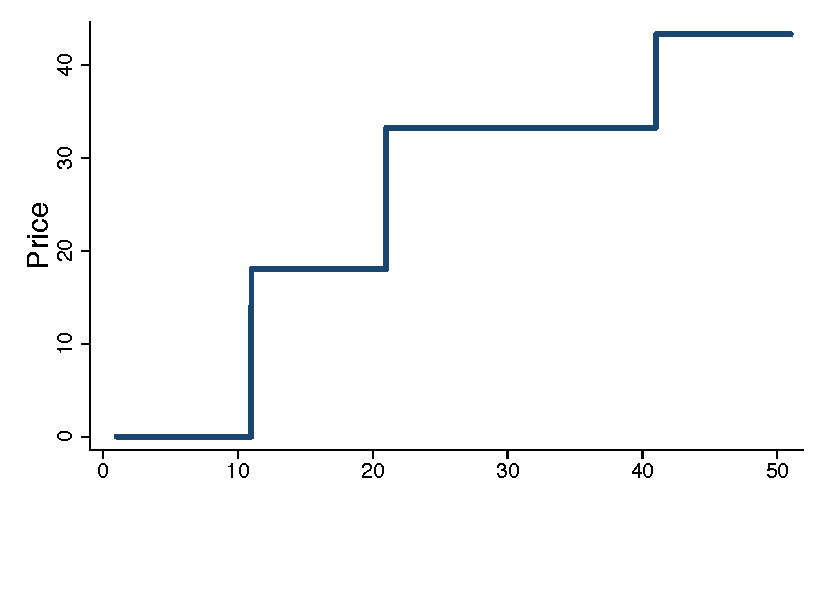
\includegraphics[width=.66\textwidth,height=1\textheight,keepaspectratio]{tables/tariff_structure_1_no_label.pdf}};

\draw [line width=0.2mm,color=red,dashed] (2.8,1.8) -- (2.8,7.6);
\draw [line width=0.2mm,color=red,dashed] (3.8,1.8) -- (3.8,7.6);
\draw [line width=0.2mm,color=red,dashed] (4.6,1.8) -- (4.6,7.6);
\draw [line width=0.2mm,color=red,dashed] (5.5,1.8) -- (5.5,7.6);
\draw [line width=0.2mm,color=red,dashed] (8.2,1.8) -- (8.2,7.6);
\draw [line width=0.2mm,color=red,dashed] (9.1,1.8) -- (9.1,7.6);

\node[align=center] at (2.7,7.6)  { \text{\footnotesize  $\overline{\eta}^{1}_{1,L} $}};
\node[align=center] at (3.7,7.6)  { \text{\footnotesize  $\overline{\eta}^{2}_{2,L} $}};
\node[align=center] at (4.5,7.6)  { \text{\footnotesize  $\overline{\eta}^{2}_{1,U} $}};
\node[align=center] at (5.4,7.6)  { \text{\footnotesize  $\overline{\eta}^{3}_{2,U} $}};
\node[align=center] at (8.1,7.6)  { \text{\footnotesize  $\overline{\eta}^{3}_{3,L}  $}};
\node[align=center] at (9,7.6)  { \text{\footnotesize  $\overline{\eta}^{4}_{3,U}  $}};

\draw [line width=0.5mm] (1.2,7.6) -- (2.8,7) -- (3.8,6) -- (4.6,4.5) -- (5.2,2); %% curve

\node[align=center] at (1.8,1)  { \text{\footnotesize  $D^{1}_C$}};
\node[align=center] at (2.8,1) { \text{\footnotesize  $D^{1,2}_C$}};
\node[align=center] at (3.8,1)  { \text{\footnotesize  $D^{1,2,3}_C $}};
\node[align=center] at (4.8,1) { \text{\footnotesize  $D^{2,3}_C $}};
\node[align=center] at (6.8,1)  { \text{\footnotesize  $D^{3}_C $}};
\node[align=center] at (8.3,1)    { \text{\footnotesize  $D^{3,4}_C $}};
\node[align=center] at (9.6,1)  { \text{\footnotesize  $D^{4}_C $}};

\node[align=center] at (2.3,2.3) { \text{$p^1$} };
\node[align=center] at (4,4.5)   { \text{$p^2$} };
\node[align=center] at (6.6,6.4) { \text{$p^3$} };
\node[align=center] at (10,7.6) { \text{$p^4$} };

\end{tikzpicture}
\end{figure}

This section now discusses the separate parts of the demand function in more detail.

\textbf{  Demand over a Single Price:  }  The first, third, and fourth price segments of the tariff schedule in Manila given in Figure~\ref{figure:intuitivedemand} exhibit large gaps of 20 $\text{m}^{3}$ between price changes.  Within these segments, the consumption shocks are not large enough to ever bounce the households across a kink point in these regions.  Therefore, households are exposed only to the current price for that segment.  Setting the low, medium, and high prices all equal to $k$ in expression $D^{L,M,H}_C$, demand arrives at the following expression:
\begin{align*}
  D_C  =& \gamma_C - \alpha_C H_{C} - \frac{\alpha_C}{S} p^k + \eta_C 
\end{align*}
This case produces a linear demand function where $\alpha_C$ can be readily interpreted as the price sensitivity parameter while $\gamma_C$ captures the portion of demand that is invariant to prices.  This demand function captures moral hazard from bill-splitting by dividing the price sensitivity, $\alpha_C$, by the total number of households using the connection, $S$.  Comparing demand among shared connections to individual connections, the extent of over-consumption at an average price of $p$ can be roughly summarized as $\frac{S-1}{S} \alpha_C p $.   

\textbf{ Demand over Many Prices: }  When households choose to consume close to price thresholds points, they become exposed to price segments both above and below the thresholds.  Demand becomes a weighted average of these two price segments.  In this case, demand takes the following form, setting low and medium prices equal to $k$, and the high price equal to $k+1$:
\begin{align*}
D_C &= \frac{ 1}{ V^{k,k+1} } \Big ( \gamma_C - \alpha_C H_{C} - \frac{\alpha_C}{2 S}  [ p^{k} + p^{k+1} - \overline{W}^{k+1} (\frac{p^{k+1} - p^{k}}{\sqrt{2}{\sigma_{\epsilon_C}}})  ]  \Big ) + \frac{ \eta_C }{ V_{k+1,k} } 
\end{align*}
Setting $L=M=k$ simplifies the demand expression so that only the single nearby kink point, $\overline{W}^{k+1}$, is considered.  Under increasing mprices, a decrease in the kink point, $\overline{W}^{k+1}$, lowers demand by increasing the probability that the household faces a higher price.

When the distance between price segments is relatively small compared to the size of the consumption shocks, then households are exposed to three prices when consuming on a particular segment.  Despite locating far from the neighboring kink points, households still face some probability of crossing into another price segment either above or below their current price.  This demand function applies to households locating between the second and third tariff blocks because this gap only spans 10 $\text{m}^{3}$ (as shown in Figure~\ref{figure:intuitivedemand}).  The demand function corresponds to the full expression for demand, setting indices for the low price equal to $1$, the middle price equal to $2$, and the high price equal to $3$.  

\subsubsection{Deriving the Likelihood Function}

Given the optimal consumption choice, $w^{*}_C$, for each connection, observed consumption for a particular connection, $Q_C$, becomes the sum of optimal consumption and the total consumption shock for that connection, $\epsilon_C$:
\begin{align}\label{equation:observeddemand}
Q_C &= w^{*}_C + \epsilon_C
\end{align}
The probability of observing any consumption outcome, $Q_C$, can be expressed as the sum of the probability that the preference shock, $\eta_C$, locates the households within a particular price segment multiplied by the joint probability that the consumption shock, $\epsilon_C$, and the preference shock are equal to $Q_C$ conditional on being in this price segment.

These probabilities allow for the derivation the likelihood function for each consumption realization, using some additional notation.\footnote{By allowing households to anticipate exogenous shocks to their consumption, this approach builds on the standard framework of \cite{burtless1978effect} and \cite{moffitt1986econometrics} to estimate demand over non-linear budget constraints, which has been recently implemented by \cite{szabo2015value} and \cite{mcrae2014infrastructure}.}  Let demand within each segment in equation (\ref{equation:generaldemand}) simplify to $D_k = D^{l_k,m_k,h_k}_C$.  Similarly, denote the variance term for each segment as $V_k = V^{l_k,h_k}$.  Given by the conditions on $\eta_C$ defining each segment in equation (\ref{equation:generaldemand}), denote the bottom threshold for the preference shock as, $\overline{\eta}_{B,k} = \overline{\eta}^{B_p,k}_{B_{\overline{W},k},B_{\sigma}}$ and the top threshold as $\overline{\eta}_{T,k} = \overline{\eta}^{T_p,k}_{T_{\overline{W},k},T_{\sigma}}$.  Define the variance-adjusted preference shock as $\Psi = \frac{\eta_C}{V_k}$.  Let the sum of the two stochastic terms equal $\zeta = \Psi + \epsilon_C$.  For any random variable, $x$, denote the cumulative distribution function as $F_x$ and the corresponding probability distribution function as $f_x$.  Also, let $\phi$ and $\Phi$ denote the standard normal p.d.f. and c.d.f. respectively.  Given equation (\ref{equation:generaldemand}), the contribution to the likelihood function for consumption observation for each connection can be written as:
\begin{align}\label{equation:llcontributionlinear}
\sum_{k} f_{\zeta}( Q - D_k ) \Big [ F_{ \Psi | \zeta = Q - D_k } (\overline{\eta}_{T,k}) - F_{ \Psi | \zeta = Q - D_k } (\overline{\eta}_{B,k})  \Big ]
\end{align}
This expression takes the sum of the densities of $\zeta$ for each consumption level weighted by the probability that the preference shock $\Psi$ locates the desired consumption level for that household between the two thresholds, $\overline{\eta}_{T,k}$ and $\overline{\eta}_{B,k}$ over all thresholds.  Given that $\eta_C$ and $\epsilon_C$ are assumed to be independent and normally distributed, the terms in equation (\ref{equation:llcontributionlinear}) can be rewritten using both the convolution and conditional distributions of multivariate normals:
\begin{align*}
f_{\zeta}( Q - D_k ) &= \frac{1}{\sigma_{\zeta,k}} \phi(\frac{Q - D_k}{\sigma_{\zeta,k}} ) \\
F_{ \Psi | \zeta = Q - D_k } (\overline{\eta}_{k}) &= \int_{-\infty}^{\overline{\eta}_{k}} f_{\Psi | \zeta = Q - D_k} (x) dx \\
&= \int_{-\infty}^{\overline{\eta}_{k}} \frac{1}{\sigma_{\zeta,k} \sqrt{1-\rho_k^2}}\phi \Big ( \big ( \frac{ x V_k}{\sigma_\eta} -  \rho_k q_{k} \big )\frac{1}{\sqrt{1-\rho_k^2}}   \Big ) dx \\
&= \Phi \Big ( \big ( \frac{\overline{\eta}_{k} V_k}{\sigma_\eta} -  \rho_k q_{k} \big )\frac{1}{\sqrt{1-\rho_k^2}}   \Big ) \\
\text{Where:} &\\
q_k &= \frac{(Q - D_k)}{\sigma_\zeta}, \hspace{.4cm}  \sigma_{\zeta,k} = \sqrt{ \frac{\sigma_{\eta}^2}{V_k^2} + \sigma_{\epsilon_C}^2}, \hspace{.4cm} \rho_{k} = \frac{ \sigma_{\eta}}{  \sigma_{\zeta,k} V_k  } 
\end{align*}
Given these terms, equation (\ref{equation:llcontributionlinear}) can be rewritten in the following way:
\begin{align}\label{equation:LLikelihood}
\begin{split}
LL &= \sum_{k=1}^{K}  \frac{1}{\sigma_{\zeta,k}} \phi (q_{k}) \Big[ \Phi \Big ( \big ( \frac{\overline{\eta}_{T,k} V_k}{\sigma_\eta} -  \rho_k q_{k} \big )\frac{1}{\sqrt{1-\rho_k^2}}   \Big ) -  \Phi \Big( \big ( \frac{\overline{\eta}_{B,k} V_k}{\sigma_\eta} -  \rho_k q_{k} \big )\frac{1}{\sqrt{1-\rho_k^2}}   \Big)\Big] 
\end{split}
\end{align}
Summing each part of the demand function in equation (\ref{equation:generaldemand}) in the likelihood expression in equation (\ref{equation:LLikelihood}) computes the probability of observing consumption outcomes for each connection.  In order to include multiple time periods, the model captures variation in consumption over time by assuming that each household receives independent draws of preference shocks, $\eta_{i,t}$, and consumption shocks, $\epsilon_{i,t}$, which aggregate at the connection-level to $\eta_{C,t}$ and $\epsilon_{C,t}$ respectively for each month, $t$.  All other parameters are assumed to remain stable over time.  The full log-likelihood is computed by summing the log of the likelihood in equation  (\ref{equation:LLikelihood}) over all connections and time periods.  


\subsubsection{Households using from Water Small-Scale Providers}

6\unskip\% of households source their water from small-scale water vendors.  These sources are collapsed into a single vendor category, which is modeled as a perfect substitute to piped water and is characterized by a monthly fixed fee, $F_v$, and a marginal price, $p_v$.  The monthly fixed fee, $F_v$, is assumed to capture primarily fixed differences in quality of service between vended water and other sources.  Similarly, the marginal price, $p_v$, includes both the price per unit as well as any differences in water quality or ease of use relative to piped water.  Demand for this source becomes a simple linear function of prices given by equation (\ref{equation:vendordemand}).
\begin{align}\label{equation:vendordemand}
w^{*} = \Gamma_i - \alpha_i p_v
\end{align}
Since the data do not record monthly consumption information for households using from vendors, these households do not contribute to the likelihood function above.  



\subsection{Water Source Choice}\label{section:watersourcechoice}

This section describes a sequential game where households choose their water sources.  This game results in a unique equilibrium of source choices given the preferences parameters for each household as well as the costs of using each water source.  This game also allows for a mapping between the fixed costs of setting up and maintaining each water source and cross-sectional variation in source choices, which informs the third step of the estimation strategy.  The fundamental assumption of this model is that the decision to share a water connection balances splitting the fixed costs among many households against facing higher marginal costs --- hassle costs in fetching water and free-rider costs splitting the water bill.

With demand for water for each household, I am able to calculate the expected utility that each household receives from each water source, guiding their source choices.  This choice becomes a strategic decision since each household's water connection can also serve as a water source for other households in a neighborhood.  The model assumes that each set of neighboring households plays a full-information, sequential game, deciding whether to purchase their own tap, share with a previously connected household, or purchase from a vendor.  Assuming a sequential order of moves acts a refinement to rule out situations with multiple equilibria.  Eliminated equilibria mainly include cases that are both strictly dominated and unrealistic such as having all households use from vendors when they would prefer to share a connection.

Let superscripts index households by the order in which they move.  Let $a^{i}$ denote the water source choice for each household $i$.  The choices consist of (1) using from a vendor, $v$, (2) purchasing a connection, $c$, or (3) sharing with neighbor, $j$, given by $s^{j}$.  The first mover faces a simple choice set defined by $A^{1} = \{  v, c  \}$.

For all other households, define the following function that maps a household's choice to connect into a sharing opportunity for the following households:
\begin{align*}
g( a^{j} ) &=
\begin{cases}
s^j        &  \text{ if } a^{j} = c \\
\emptyset  &  \text{ else } 
\end{cases}
\end{align*}
Given this function, the choice sets for households $i>1$ consist of $A^{i} = \{ v,c,g(a^{1}),...,g(a^{i-1}) \} $ where households only have the option to share with neighbors that have previously connected.  

The payoffs equal the expected utilities from each source over the duration of usage.  Since the data do not measure the exact duration for which households reside in a location using a water source, the model includes two additional assumptions: (1) households do not discount their future utilities and (2) all households demand water for an equal number of months.  These assumptions limit the extent to which this model can examine the timing of any one-time connection fees or other upfront costs of water connections.  Instead, the model collapses one-time fees into a single monthly fixed fee.  Any heterogeneity in either the duration of demand or discount factors is captured by estimates of this monthly fixed fee.  
%This section now describes the payoffs in more detail.
%% Potential limitations of this approach are discussed in more detail in the estimation section.

To compute the payoffs from using vended water, households simply compute their expected utility given by equation (\ref{equation:umaxfirst}) according to their demand in equation (\ref{equation:vendordemand}).  Let $u^{i}(v)$ capture this payoff.

The payoff from owning a connection depends on whether other households choose to use the connection as well.  Households are assumed to have perfect information about each other's preferences including distributions of preference and consumption shocks.  In order to calculate surplus from sharing, let the set $S^{i}$ contain all households that have chosen to use household $i$'s connection (including the owner).  In this model, sharing affects the utility of the owner in three ways.  First, increasing the number of sharing households splits the total water bill over more households, exacerbating any moral hazard distortions as illustrated in equation (\ref{equation:generaldemand}).  Second, under non-linear tariffs, including more consumption on the same connection may alter the marginal prices faced by all sharing households.  

Third, in this model, owning households ($i=1$) are assumed to pay the full fixed cost, $F$, and sharing households commit ex-ante to providing a fixed transfer to the owner each month to compensate the owner.  This transfer allows sharing households to help contribute to the fixed costs of owning and maintaining the connection.  60\unskip\% of sharing households in the mobile survey report splitting some or all of the initial connection fee with their neighbors; for the remaining share, the owner pays the full connection fee.  

To capture this behavior, the model assumes that sharing households offer transfers to the owner which equally split their surpluses from using the connection.  This setup is analogous to a Nash-Bargaining framework with equal bargaining weights.  While the division of surplus does not affect the efficiency of sharing relationships, it has normative implications for the types of households that are able to benefit from these arrangements.  Three features of the context in Manila support this assumption of a roughly equal division of surplus.  First, these sharing arrangements feature long-term relationships between close neighbors who are also often family members.  Second, neighborhoods often feature multiple sharing opportunities for each household, creating some competitive pressure on sharing arrangements.  Third, in the mobile survey, sharing households appeal to an ethic of fairness as the primary reason for dividing monthly payments instead of other reasons such as matching tariff prices or conserving environmental resources.

Expected utility from using a connection alone is defined as $u^{i} (c|1)$.  This expression can be computed by inputting demand from equation (\ref{equation:generaldemand}) with $S=1$ into utility given by equation (\ref{equation:umaxfirst}).  Expected utility from owning and sharing a connection is defined as $u^{i}(c | S^i ) $ and expected utility for household $j$ from using a connection owned by neighbor $i$ as $u^{j} ( s^{i} | S^i )$.  
%Sharing utilities can be calculated with the same method, substituting for $S$.

Sharing surplus for the owner of the connection can be represented as $ O^{i} = u^{i} ( c | S^{i} ) - max \{ u^{i} (c | 1), u^{i}(v) \} $ while surplus for each other sharing household $j$ takes the form $ G^{j} = u^{j} ( s^{i} | S^{i} ) - max \{ u^{j}(c | 1), u^{j}(v) \} $.  Let $t_{j}(S^{i})$ denote the transfer from sharing household $j$ to the owning household $i$.  Following the outcome of a Nash-Bargain with equal weights, define $  t_{j}(S^{i}) = \frac{S^{i}-1}{S^{i}} G^{j}  - \frac{1}{S^i} O^{i} - \sum_{k \in  S^{i} \setminus \{ 1,j \} } \frac{1}{S^i} G^{k}  $.  The total transfer that the owner receives from all sharing partners equals $T (S^{i}) = \sum_{j \in S^{i} \setminus \{ 1 \} } t_{j} (S^{i})$.  For example, when only two households use the connection, then $T(\{1,2\}) = t_{2}(\{1,2\}) = \frac{1}{2} (G^2 - G^{1})$, which simply divides the surplus in two.  While these transfers are usually positive since the owner is assumed to shoulder all of the fixed costs of maintaining a connection, there may be cases where the owner will offer payment to other households to use their connection: for example, if the owner has a much larger demand for water than other users, the owner may benefit substantially from splitting the bill evenly with these other households.  This case would be captured through a negative transfer.  

From a welfare perspective, these transfers help to ensure that households form efficient sharing relationships.  For example, transfers allow neighbors to incentivize others to purchase a connection in cases when owners would not otherwise be willing to own and share a water connection.  Transfers also serve to reconcile a tension introduced by the sequential structure of the game where a first mover may be compelled into a sharing relationship by a second mover although the first mover would rather use the connection alone.  Transfers eliminate this possibility by calculating surplus from sharing relative to the maximum expected utility from using a vendor or using a water connection alone.  

Given these transfers, the payoff for household $i$ choosing to connect takes the form $u^{i} (c|S^{i}) + T(S^{i})$.  Meanwhile, the payoff for household $j$ sharing a connection with household $i$ is $u^{j} (s^{i}|S^{i}) + t_{j}(S^{i})$.  Both the past and future decisions of all other households enter these payoffs by determining the resulting set of sharing households, $S^{i}$, which affects expected utilities directly as well as through transfers.

The last step in the specification of this game is determining the order in which households choose water sources.  The model sequences households according to their expected net utility from owning a connection alone relative to using from a vendor, $u^{i}(c|1) - u^{i}(v)$.  This arrangement matches the intuition that households with the greatest incentives to own and maintain a water connection would likely be the first to purchase a connection.  Table~\ref{descriptives} shows that for connections serving two households, the owner's household size is 8\% larger than the buyer's household size on average.  To the extent that household size serves as a proxy for demand, this finding provides suggestive evidence that larger demand households with greater utility from purchasing a water connection are also more likely to be owners.  Given that transfers allow households to efficiently share surplus, the sequence is unlikely to have large impact on the overall efficiency of the resulting arrangements.  However, moving earlier may affect the welfare of particular households.  On one hand, early movers can select to join high-value sharing relationships, crowding out these opportunities for later movers.  On the other hand, later movers have a broader choice set of already-connected households to establish a sharing relationship.

The sequential game is solved using backward induction and considering only pure-strategy equilibria.  First, the last mover, household $I$, identifies the choices that maximize its payoffs at each possible choice set reached by the game.\footnote{In rare cases where payoffs are equal, the tie-breaking rule prioritizes vendors, then individual connections, and finally shared connections ranked by the sequence of owners.}  Given these choices, the next-to-last mover, household $(I-1)$, can calculate its payoffs for each corresponding choice set.  Iterating backwards, this process characterizes a unique equilibrium set of source choices for all households.  Appendix Figure~\ref{figure:fullgametree} provides an extensive form for the game that is simulated in this paper.


\subsubsection{Exogenous Interruptions to a Water Source}\label{section:hasslemodel}

This section describes an extension of the model to allow for exogenous interruptions in a water source that induce households to substitute toward another water source.  Exogenous interruptions produce useful variation in the types of water sources used by each household, serving an important role in estimating the hassle costs of transporting water from a neighbor.  Due to shifts in the geology, road construction, or aging infrastructure, households sometimes experience underground breaks in the service pipe between the main line and the water meter.  These leaks result in repair costs and water bills borne by households that can be large enough to force affected households to switch to an alternative water source.

Descriptive evidence suggests that the decision process to choose an alternative water source in response to a leak is much different from the initial choice households face in deciding on a long-term water source.  The mobile survey asks households which source they would substitute towards if they were to be disconnected for at least three months.  30\unskip\% report that they would ``use a neighbor's tap'' while the remaining responses are roughly evenly split between using a public or private deep well, fetching from a water truck, or filling bottles at a water refilling shop.  Although shared connections vastly outnumber households using from vendors in the population as shown in Table~\ref{descriptives}, using a neighbor's tap is less common in response to a sudden disconnection.  Since sharing relationships often take the form of long-term contracts, households may often face high costs in reaching a temporary sharing agreement with a neighbor.  Additional descriptive findings discussed in Section~\ref{section:hasslecostestimation} suggest that the decision to share with a neighbor is uncorrelated with the features of water demand among both the household experiencing a leak as well as their neighbors.  These patterns indicate that substitution may be driven less by minimizing the long-term costs of using each source and more by convenience such as immediate access or relationships between neighbors.

From the perspective of the sequential game, households experiencing leaks are assumed to be last-movers, which implies that other households cannot update their water source choices in response to a neighbor's leak.  Additionally, the model assumes that households do not anticipate any risks of leaks in making their initial connection decisions.  Since leaks are relatively rare events as discussed in Section~\ref{section:hasslecostestimation}, this assumption is unlikely to significantly affect predicted water source choices.  

Let $l$ index households experiencing a leak while $j$ indexes connections in the same neighborhood (reaching a total of $J$ connections).  This model deviates from the initial water source choice by assigning an idiosyncratic preference term, $\xi_{A,l}$, to each alternative water source $A$ --- either using from a vendor, $v$, or sharing with a neighbor, $s^{j}$.  $\xi_{A,l}$ captures the convenience of temporarily using each source following a sudden loss of water access.  For example, the first term, $\xi_{A,l}$, may capture idiosyncratic, easy access to a neighbor's private deep well or a water refilling station.  Similarly, the second term, $\xi_{A,l}$, might measure the relative social capital among potential sharing partners: nearby family members may be more willing to quickly share their connection.  The model also includes the term $F^{S}$ to capture any fixed costs associated with setting up a temporary sharing relationship relative to simply fetching from a vendor.  Given these preference shocks, total utility for household $l$ for using alternative $A$ can be parameterized with the following:
\begin{align}\label{equation:hassleutilities} 
\begin{split}
U_{l}(A) &= \omega u_{l}(A) - \mathbbm{1}\{ A \neq v \} F^{S}  + \xi_{A,l} \\
A & \in \{v,s^{1},...,s^{J}\}
\end{split}
\end{align}
$F^{S}$ captures the relative substitution to sharing relationships and to water vendors.  This model includes the additional assumption that $\xi_{A,l}$ is distributed Type I Extreme Value and is independent of preferences for water usage.  Under the distributional assumptions, the model predicts that conditional on choosing a sharing relationship, households evenly distribute between sharing partners as $\omega$ approaches zero.  When $\omega$ equals zero, the probabilities of households choosing each alternative source simplify to the following:
\begin{align*}
Pr[A=v] &= \frac{e^{-F^{S}}}{e^{-F^{S}}+e J} = G \\
Pr[A=s^{j}] &= \frac{e}{e^{-F^{S}}+eJ} = \frac{(1-G)}{J}  \\
\text{ for } j &= 1..J
\end{align*}
Let $L$ represent the total households affected by a leak.  $L$ is greater than one in cases where connections serving multiple households experience a leak.  All $L$ households are assumed to receive the same preference shock $\xi_{leak,A}$ so that they follow identical substitution patterns.  This assumption may lead to a slight underestimation of the hassle costs since these households may actually distribute across different sharing relationships, exposing them to lower points on the tariff schedule than if all households were clustered on the same connection.

These assumptions allow for the specification of a likelihood function that expresses neighbor's consumption following a leak as a function of household preferences and the hassle cost, $p_h$.  Define $LL(\gamma,\alpha,S)$ as the likelihood function in equation (\ref{equation:LLikelihood}) in terms of the preference parameters--- $\gamma$ and $\alpha$ --- as well as the number of households using the connection, $S$.  Given the probabilities above, the likelihood for consumption from connection $j$ after a nearby leak can be expressed as follows:
\begin{align}\label{equation:hasslelikelihood}
\begin{split}
LL_{j,Post l} = & \frac{J-(1-G)}{J} \overbrace{LL(\gamma_j,\alpha_j,S_j)}^{\text{$L$ do not share with $j$}} + \\
	    & \frac{(1-G)}{J}  \underbrace{LL(\gamma_j + \gamma_{L},\alpha_j+\alpha_{L},S_j+S_L)}_{\text{$L$ share with $j$}}
\end{split}
\end{align}
The first term multiplies the standard likelihood for this connection by the probability that households $L$ do not share with connection $j$.  The second term adds the probability that $L$ households choose to share with connection $j$ following the leak.  This probability is multiplied by the likelihood corresponding to joint consumption, which includes both preference terms from connection $j$ as well from $L$ households.  This approach recovers the hassle cost, $p_h$, by comparing the fixed preferences for households experiencing the leak before and after they start using from a neighbor.  Let $pre$ take a value of one for months before a leak.  Fixed preferences for $L$ households take the following form:
\begin{align*}
\gamma_{L} = &  \sum_{l=1}^{\overline{L}} ( \gamma_{l} - \alpha_{l} P_{h,l} ) \\
P_{h,l} = & 
	\begin{cases}
	0     &  \text{ if } l=1 \text{ and } pre=1 \\
	p_h   &  \text{ else }
	\end{cases}
\end{align*}
Substituting to a neighbor's connection newly exposes the owner, $l=1$, to the hassle cost $p_h$ while other households $s \neq 1$ are assumed to be exposed to the hassle cost both before and after the leak.  Therefore, this method identifies hassle costs from variation in exposure for owners of the connection.  Section~\ref{section:hasslecostestimation} details potential limitations of this assumption.


















\section{Specification and Estimation}\label{section:specificationandestimation}

The estimation strategy takes place in three steps.  In the first step, preference parameters --- fixed preferences $\gamma$, price sensitivities $\alpha$, as well as variances for the consumption and preference shocks, $\sigma_{\epsilon}$ and $\sigma_{\eta}$ respectively --- are recovered by combining monthly consumption patterns with price variation.  The second step analyzes a quasi-experiment where households are exogenously switched from individual connections to shared connections to estimate the hassle cost, $p_h$, associated with sharing.  In the third step, monthly fixed costs associated with an individual connection, $F$, and using a water vendor, $F_{V}$, as well as the marginal price from vendors, $p_V$, are chosen to best match cross-sectional moments in the data, including the shares of households choosing each source.

\subsection{Preference Estimation}\label{section:preferenceestimation}

Household preferences for water are estimated by maximizing the likelihood function in equation (\ref{equation:LLikelihood}) for consumption recorded at each connection and month.  This section first details how each set of parameters are parameterized in the estimation:

\textbf{Fixed Preferences} $\hat{\gamma_C} = (\gamma_C - \alpha_C H_C)$  :  Since consumption data is recorded for connections rather than for households, this approach estimates a separate $\hat{\gamma_C}$ for each connection from the mean observed usage for each connection.  $\hat{\gamma_C}$ includes not only the total fixed preference parameters for households sharing a connection $\gamma_C$, but also any hassle costs faced by shared households weighted by the price sensitivity, $\alpha_C H_C$.  Since hassle costs do not vary over time or with prices, they are indistinguishable from fixed preferences for consumption in this step of the estimation.  I later decompose these estimates into household-level preferences as detailed in Section~\ref{section:fixedcostestimation}.

\textbf{Price Sensitivity} $\alpha_C$  :  The estimation parameterizes household price-sensitivity terms $\alpha_i$ as a linear function of a vector of observable characteristics $Z_i$ that may affect price sensitivity so that $\alpha_i = \alpha Z_i$.  $Z_i$ includes dummy variables for household size, type of dwelling, whether a household member is employed in a low-skilled industry, number of employed household members, and age of the head of household as shown in Table~\ref{table:demandestimates}.\footnote{For shared connections, the data include information on household size separately for owners and sharing households; however, the other observables are recorded only for owners.  For these owner-specific measures, the estimation simply assigns the owner's characteristics to sharing households.  While this imputation may be reasonable for spatially correlated characteristics like type of dwelling, this approach may introduce bias if sharing households have systematically different levels of employed individuals or ages.  Estimates of $\alpha$ in Table~\ref{table:demandestimates} exhibit little heterogeneity across many of these dimensions, which suggests that any bias from mismeasurement may have small effects on the counterfactual exercises.}  Since household-specific price sensitivities $\alpha_i$ enter linearly into the connection-level demand function in equation (\ref{equation:generaldemand}), connection-level price sensitivity can be written simply as $\alpha_C = \alpha \sum_{i=1}^{S} Z_i$.\footnote{The model does not control for seasonality or calendar time since the raw data exhibit negligible trends in water usage over time.}

The empirical setting in Manila provides a broad range of price variation to identify these price sensitivity terms separately from the fixed preferences.  First, the non-linear pricing structure given by Figure~\ref{figure:tariff} forces households to decide whether to consume above or below tariff kink points as they face monthly shocks to their demand.  Second, regulated tariff changes over time affecting all households generate time-series variation in the tariff, which can be seen in Appendix \ref{appendix:tariffvariation}.  Third, I use rate-changes which affect individual connections differently over time described in more detail in Appendix~\ref{appendix:ratechangeelasticity}.  The structural model combines all of these sources of price variation in the estimation.  The identification assumption is that the consumption and preference shocks, $\epsilon,\eta$ are uncorrelated with these price changes.

\textbf{Preference and Consumption Shocks} $\sigma_{\eta},\rho_{\eta},\sigma_{\epsilon},\rho_{\epsilon}$  :  This strategy also estimates parameters governing the distribution of preference and consumption shocks.  

%Household-level preference shocks $\eta_i$ can be aggregated to a connection-level preference shock $\eta_C$ which is composed of both the standard deviation of the $\eta_i$ terms as well as the extent to which these terms are correlated between sharing households.  
The estimation strategy recovers connection-level variance terms $\sigma_{\eta}$ for different types of connections, which are later decomposed into household variance and covariances between neighboring households below.  Heterogeneity in $\sigma_{\eta}$ is estimated with respect to connections serving one, two, or three plus households.  The estimation also allows $\sigma_{\eta}$ to vary non-parametrically according to quintiles of mean consumption at the connection-level.  Since larger users naturally have higher variance in their consumption, estimating a single $\sigma_{\eta}$ across all connections produces a large bias in the price sensitivity coefficients, $\alpha$.  This bias results from constraining large and small users to receive similarly scaled shocks and therefore enforcing that these users respond to the non-linear tariff schedule in similar ways.  While using quintiles of observed consumption may be problematic since consumption choices are themselves endogenous, this approach approximates connection-specific, $\sigma_{\eta}$ terms, which would be infeasible given limited months of data available for each connection.  The results are robust to different non-parametric specifications for $\sigma_{\eta}$.  

Following a similar strategy, the estimation recovers separate standard deviation terms at the connection-level for consumption shocks $\sigma_{\epsilon}$ according to the number of households using each connection.  Since consumption shocks exhibit little heterogeneity with respect to observed consumption quintiles, I exclude these terms from the estimation to preserve parsimony.

The $\sigma_{\eta}$ and $\sigma_{\epsilon}$ parameters are separately identified from the extent of clustering around price thresholds relative to the overall variance of consumption.  Greater clustering near price thresholds implies that households face small consumption shocks, allowing them to accurately target price thresholds and lowering estimates of $\sigma_{\epsilon}$.  Similarly, wide variance in overall consumption is attributed to large consumption shocks, increasing estimates of $\sigma_{\eta}$.  Identification for these parameters as well as the preference parameters also relies heavily on the distributional assumptions of normality.

To recover the correlations of preference and consumption shocks between neighboring households given by $\rho_{\eta}, \rho_{\epsilon}$, this method compares the estimates of $\sigma_{\epsilon}$ and $\sigma_{\eta}$ according to the number of households using each connection.  This approach assumes that household-level shocks are drawn from distributions with the same standard deviations --- $\sigma_{\eta}$ and $\sigma_{\epsilon}$.  Under this assumption, any differences in estimated standard deviations for connections serving different numbers of households can be attributed to correlations in shocks between households in the same neighborhood.  Ordering households according to the sequential game in Section~\ref{section:watersourcechoice}, let the correlation terms between the first-mover and any other households in the neighborhood, $\rho_{l,1}$, be determined in terms of the following expression where the second subscripts on the $\sigma$ terms index the number of households using a connection:
\begin{align*}
\rho_{l,1} &= \frac{\sigma_{l,2}^2 - 2\sigma_{l,1}^2}{2\sigma_{l,1}^2} \text{ for } l =  \eta, \epsilon 
\end{align*}
The next expression extends this framework to identify the correlation between the second mover and all other households in a neighborhood:
\begin{align*}
\rho_{l,2} &= \frac{\sigma_{l,3}^2 - 3\sigma_{l,1}^2- 4 \rho_{l,1} \sigma_{l,1}^2 }{2\sigma_{l,1}^2 } \text{ for } l =  \eta, \epsilon
\end{align*}
Although sharing relationships and neighborhoods are limited to a maximum of three households in this paper, this approach can be used to identify correlations between an arbitrary number of sharing partners.

\textbf{Sample} : The estimation uses a 10\% sample of connections from the connection survey (5,000 connections), which serves as the primary sample for the counterfactual exercises.  This sample is combined with 5,239 connections from the leak quasi-experiment used in Section~\ref{section:hasslecostestimation}, which takes preference estimates from this step as an input.  Together these connections produce 473,114 months of consumption observations used in the preference estimation.  All standard errors throughout this paper are bootstrapped using 60
repetitions.  This sample does not include households using water from vendors since the data do not include information on consumption for these households.  Section~\ref{section:fixedcostestimation} details the imputation procedure used to infer preferences for these households.  Appendix~\ref{appendix:sigmanuassumptions} determines the ex-ante assumptions on $\sigma_{\epsilon}$ needed to identify the particular demand function.
%The estimates are robust to varying the total and relative sample sizes of these groups.

\textbf{Estimates} : Table~\ref{table:demandestimates} provides estimates for the different parameters as well as bootstrapped standard errors.  The price sensitivity parameter, $\alpha$, exhibits some statistically significant heterogeneity across demographic measures although the magnitudes of these estimates are relatively small compared to the intercept.  Moderately sized households have larger price sensitivities while employment among household members tends to lower price sensitivity estimates.  Relative to living in a duplex, households in apartments and single houses exhibit greater price sensitivities with large standard errors.  These estimates can be difficult to interpret economically since the elasticity of demand depends not only on these $\alpha$ terms, but also on variation in the fixed preferences for water across households.

Estimates of the variance of consumption shocks, $\sigma_{\epsilon}$ increase slowly as the number of households using a connection increases.  This finding provides suggestive evidence that shocks to sharing households may be negatively correlated.  The standard deviation of preference shocks, $\sigma_{\eta}$, increases dramatically with quintile of water usage.  After controlling for quintile of water usage, increasing the number of households per connection has a very small effect on the term, $\sigma_{\eta}$.

\begin{table}
\centering
\caption{Demand Estimates}\label{table:demandestimates}
\begin{tabular}{lcc}
& Estimate & Standard Error \\
Price Sensitivity : $\alpha$ & \multicolumn{2}{c}{}\\
\hline
Intercept &0.83&0.09\\
HHsize 4 to 5 &-0.021&0.044\\
HHsize over 5 &-0.098&0.053\\
Apartment &-0.036&0.052\\
Single House &0.051&0.043\\
Low Skill Emp. &0.016&0.053\\
Over 2 Empl. Members &0.023&0.042\\
$\alpha$: HH Head 36 to 52 years  &0.078&0.043\\
$\alpha$: HH Head over 52 years  &0.132&0.052\\
\multicolumn{3}{c}{} \\
Consumption Shock : $\sigma_{\epsilon}$ & \multicolumn{2}{c}{}\\
\hline
Single HH &4.10&0.07\\
Two HHs &5.30&0.18\\
Three HHs &5.78&0.30\\
\multicolumn{3}{c}{} \\
Preference Shock : $\sigma_{\psi}$ & \multicolumn{2}{c}{}\\
\hline
Intercept &13.31&0.45\\
Below 1st Quintile Usage &-2.99&0.28\\
Over 3rd Quintile Usage &2.82&0.30\\
Two HHs &-0.44&0.43\\
Three HHs &1.13&0.52\\
\hline
\end{tabular} 
 \\
\vspace{.1cm}
{\footnotesize{Total Observations:  349,265   Total Connections:  7,151} }
\end{table}
To interpret these estimates in economic terms, I compute the elasticity of demand with respect to price at the connection-level.  Given a linear demand structure, the elasticity of demand depends on both the price sensitivity and fixed preferences for water.  As a simplified example, consider the calculation for elasticity under a single marginal price and linear demand specification:
\begin{align*}
\frac{\delta Q}{\delta P} \frac{P}{Q} = \alpha_{C} \frac{P}{\gamma_{C}-\alpha_{C} P}
\end{align*}
According to this expression, increasing the fixed preference for water consumption, $\gamma_C$, while holding constant the price sensitivity, $\alpha_C$, mechanically reduces the elasticity.  Many previous studies estimate heterogeneity in $\gamma_C$ alongside a single $\alpha_C$ parameter for the population (\cite{mcrae2014infrastructure}, \cite{olmstead2009reduced}, \cite{szabo2015value}).  This paper builds on these previous studies by estimating heterogeneity in both terms to allow to for a broader range of possibilities, including that larger users may be relatively more sensitive to prices than smaller users.  To compare estimates in this paper with previous papers under non-linear pricing schedules, this approach follows the same formula for computing elasticities by (1) taking draws of $\epsilon$ and $\eta$, (2) computing predicted demand under prices that are 1\% greater than current prices, and (3) comparing the average percentage change in demand before and after the price change.  For tariff blocks equal to zero, prices are increased from 0 to 1 PhP following \cite{szabo2015value}. 

Table~\ref{table:elasticity} presents demand elasticity estimates across terciles of (1) imputed income for the connection owner and (2) average monthly usage for the connection.  Elasticities exhibit little heterogeneity across imputed income levels, but substantial variation across usage levels with larger users appearing much less sensitive to prices than smaller users.  Since many low-income households share connections with neighbors, there is a weak correlation between income and usage-levels, which helps account for these patterns of heterogeneity.\footnote{Noise in the income imputation process may also weaken any correlation between elasticity and income.}  Heterogeneity in elasticities according to monthly usage is consistent with moral hazard when households share a connection:  increasing the number of households per connection increases the water use for those connections while also exacerbating free-riding behavior.  Different water using activities across the water demand profile may also produce this heterogeneity in elasticities.  This heterogeneity provides a potential motivation for usage-based price discrimination.  For example, matching larger, less price-sensitive users with higher prices may allow for a more efficient allocation of water while covering costs of production.

\begin{table}
\centering
\caption{Elasticity Estimates}\label{table:elasticity}
\begin{tabular}{lcc}
& Estimate & Standard Error \\
Mean Elasticity &0.778&0.106\\
\hline
 & &  \\
Elasticities by Income Tercile & & \\
\hline
Low Income &0.797&0.188\\
Medium Income &0.793&0.171\\
High Income &0.746&0.170\\
 & &  \\
Elasticities by Usage Tercile & & \\
\hline
Low Usage &1.271&0.213\\
Medium Usage &0.717&0.147\\
High Usage &0.634&0.135\\
\hline
\end{tabular} 
 \\
\vspace{.5cm}
{\footnotesize Total Observations:  349,265   Total Connections:  7,151 \\
Standard errors are bootstrapped at the connection level.}
\end{table}

The demand estimation yields an average elasticity of -0.78\unskip, which can be interpreted as the percentage change in quantity due to a one percentage change in price.  This estimate also closely matches reduced-form elasticity estimates from price-change quasi-experiment detailed in Appendix~\ref{appendix:ratechangeelasticity}.  This estimate is well below the -0.98 estimate of \cite{szabo2015value} but in the range of other similar studies in developing world that find elasticities between -0.01 and -0.81 (\cite{diakite2009proposal}, \cite{strand2005water}).  

\begin{figure}
\caption{Comparing Predicted and Observed Water Use}\label{figure:predictedwateruse}
\begin{center}
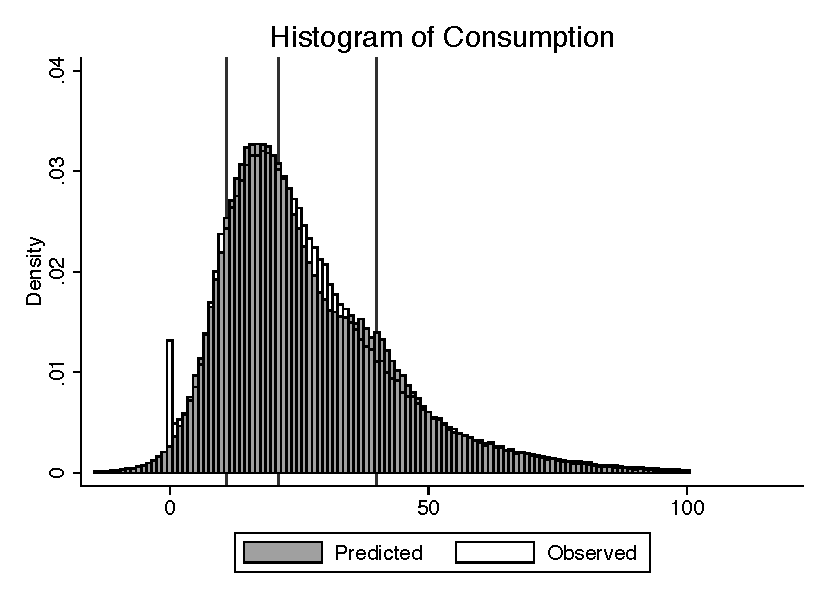
\includegraphics[scale=.77]{tables/hist_both.pdf}
\end{center}
\end{figure}

Figure~\ref{figure:predictedwateruse} compares the predicted histogram of consumption with observed values.  Vertical red lines indicate the price thresholds in the tariff schedule.  By roughly matching the smoothness of the distributions especially across price thresholds, this model improves on standard models in the literature, which often predict excessive bunching at thresholds (\cite{mcrae2014infrastructure}, \cite{olmstead2009reduced}, \cite{szabo2015value}).  The model has difficultly rationalizing low levels of consumption likely because households face zero prices below this threshold.\footnote{Since preference and consumption shocks are assumed to be normally distributed, the model predicts a handful of negative consumption values.  In the counterfactual exercises, I round these negative realizations to zero consumption.}  Likewise, the model also cannot account for bunching at zero (likely capturing households that go on vacation).  The model also predicts greater bunching around the upper price threshold despite little observed bunching in the data as large users tend to ignore this smaller jump in price.


Table~\ref{table:correstimates} presents correlation estimates decomposed from the standard deviation terms.  Both $\epsilon$ and $\eta$ shocks demonstrate negative correlations between neighbors for both first-movers and second-movers.  This finding suggests that neighboring households may intentionally form sharing relationships with whom their shocks are negatively correlated.  This behavior may provide an insurance benefit in the presence of non-linear prices, reducing the risk that joint consumption exceeds price thresholds each month.  Alternatively, these negative consumption findings may stem from households that frequently travel ensuring that at least one user is home to take care of the connection.  For example, given the high rate of overseas workers from the Philippines, it may be common for households to match with other households with different work schedules.  
%Since I have no information on the overseas work status of individuals, I am not able to test this hypothesis empirically.

\begin{table}
\centering
\caption{Correlation Estimates}\label{table:correstimates}
\begin{tabular}{lcc}
& $\epsilon$ & $\eta$ \\
\hline
Corr. Owner-Buyer: $\rho_{O,B}$ &-0.17&-0.35\\
  & (0.06) & (0.07) \\
Corr. Buyer-Buyer: $\rho_{B_1,B_2}$ &-0.17&0.21\\
 & (0.16) & (0.12) \\
\end{tabular}
\\
%\vspace{.3cm}
%\footnotesize{1 indexes correlations with first movers \\ while 2 indexes correlations with second movers}
\end{table}




\subsection{Hassle Cost Estimation}\label{section:hasslecostestimation}

This section details how exogenous interruptions in water connections caused by leaks combine with billing records to provide a measure of hassle costs of sharing water.  The estimation strategy compares a connection's demand before disconnection to the change in demand among neighboring connections after disconnection (as a result of sharing), attributing the extent to which neighbors may not fully offset their consumption to the hassle cost, $p_h$.  Baseline preference parameters for both disconnecting connections and their neighbors are estimated in the procedure from Section~\ref{section:preferenceestimation}.  Given preference parameters estimated in Section~\ref{section:preferenceestimation}, the estimation chooses the level of hassle cost, $p_h$ that best maximizes the likelihood function given in equation (\ref{equation:hasslelikelihood}).  

I now describe how the estimation sample is constructed.  In 36 months, the water provider received 106,171 complaints of excessive billing --- 34,927 of which can be precisely identified as underground pipe leaks along the service pipe through a text analysis of call transcripts.  These complaints do not appear to be spatially correlated with only a handful of leaks occurring among neighbors in the 36 months.  I consider any call identified as an excessive billing complaint as a leak.  While some calls may not explicitly refer to leaks, in all cases these calls refer to billing errors, meter malfunctions, or other surprise events that may drive disconnection.  Instances where leaks in main water pipes reduce access for entire neighborhoods at a time are coded separately and excluded from the sample.  Leaks are limited to cases with at least 3 observations before the leak in order to calculate baseline water demand for these connections.  Disconnection is defined as having 0 or missing consumption values for at least 90\% of the year following the leak date.  Neighboring connections that connect after the leak has taken place are dropped, since these connections lack a pre-period to estimate their fixed preference for water.  The estimation includes observations within a year and a half of the leak event to avoid bias from possible reconnection of these households as well as changes in the composition of neighboring households.  Since many of these households are not included in the connection survey, demographic characteristics as well as sharing behavior are imputed using averages from small areas surrounding these connections; this process introduces additional noise into the estimation.

To determine which neighbors to include, Appendix~\ref{appendix:sharingneighbor} ranks nearby households according to their distance from the leak and examine how the responsiveness of neighbors' consumption levels after a leak dissipates with distance.  Results indicate substitution is concentrated among the nearest four neighbors.  Given these findings, the empirical exercise defines neighbors as the four closest connections.  

%\footnote{Neighbors ranked 6 through 8 are grouped together since there are very few of them in the radius.}

Given the set of leaking households, $J=4$, as well as their preferences, the final input to the likelihood function in equation (\ref{equation:hasslelikelihood}) is the probability that leaking households choose to use from vendors.  This probability is calibrated directly from the hypothetical question in the mobile survey, which finds that 70\% of households would use a vendor in response to a sudden disconnection for over three months.  Directly including this parameter in the estimation requires the assumption that this hypothetical response provides an accurate measure of true behavior.

This analysis requires the assumption that the hassle cost, $p_h$, is homogenous across all households.  This assumption ensures that the hassle cost identified from the subset of leaking households can be extended to the population of households.  One concern may be that heterogenous hassle costs induce households to select into sharing relationships conditional on these costs.  Since households included in this quasi-experiment have selected into purchasing connections at baseline, they may face higher hassle costs compared to households that select into sharing.  Therefore, this exercise provides an upper-bound on hassle costs for the population.  The mobile survey finds a range of sharing access from fetching with containers to using the same plumbing, which suggests that households face different hassle costs.
The following additional assumptions are required to ensure that this empirical setting accurately captures the model described in Section~\ref{section:hasslemodel}.  These assumptions are discussed in more detail and tested empirically in Appendix~\ref{appendix:sharingcostassumptions}.
\begin{enumerate}
	\item \textit{ Connections that experience a leak are representative of the population of connections. } 
	\item \textit{ The decision to disconnect conditional on experiencing a leak is uncorrelated with water demand. } 
	\item \textit{ The timing of a leak is uncorrelated with any underlying changes in demand. } 
	\item \textit{  The leaking household's choice of a sharing partner is uncorrelated with that partner's water demand.  }	
	\item \textit{ Leaks are uncorrelated with changes in neighborhood demand. }
	\item \textit{  A leak for one household is uncorrelated with probability of a neighboring household experiencing a leak. }
\end{enumerate}

%%% ELABORATE ON ALL THE CAPTIONS TO MAKE THE FIGURES RELATIVELY SELF-CONTAINED!

Table~\ref{table:step2estimates} shows the estimation results for the hassle cost estimation.  The hassle cost is estimated to be 15.93PhP per cubic meter of usage, which is approximately 63.7\unskip\% of the average tariff.  With only 548 connections that experience leaks, the estimation recovers wide standard errors for this estimate.\footnote{Since Steps 2 and 3 of the estimation rely heavily on estimated preference terms, $\gamma$, from Step 1, Appendix~\ref{appendix:incidentalparametertest} tests for bias due to noisy estimation of these incidental parameters and finds little evidence of significant bias.}  These results suggest that the time-costs or other physical challenges transporting water to share with a neighbor may play an important role in the extent to which households choose to use water from a neighbor's tap.

%, rejecting a hassle cost of zero with 10\% confidence

%One possibility may be that estimating a single average hassle cost for the population of connections masks significant heterogeneity across household density and dwelling type among other factors.\footnote{Future versions will estimate this heterogeneity directly.}

\begin{table}
\centering
\caption{Hassle Cost Estimates}\label{table:step2estimates}
\begin{tabular}{lccc}
Hassle Cost (PhP/m3) & Sample Mean & Estimate & Standard Error \\
\hline
Intercept & 1 &-50.98 &32.79\\
\% HHs in Single Homes  &0.86&39.67&37.99\\
Avg. Distance Between HHs &1.87&17.59&6.24\\
\hline
\end{tabular} 
 \\
\vspace{.2cm} 
\footnotesize{Leaking Connections:  548,   Neighboring Connections:  2,151,   Total Obs:  20,299  \\ Standard errors are bootstrapped at the leaking connection-neighborhood level. }
\end{table}

\begin{table}
\centering
\caption{Predicted Hassle Cost Distribution}\label{table:step2histogram}
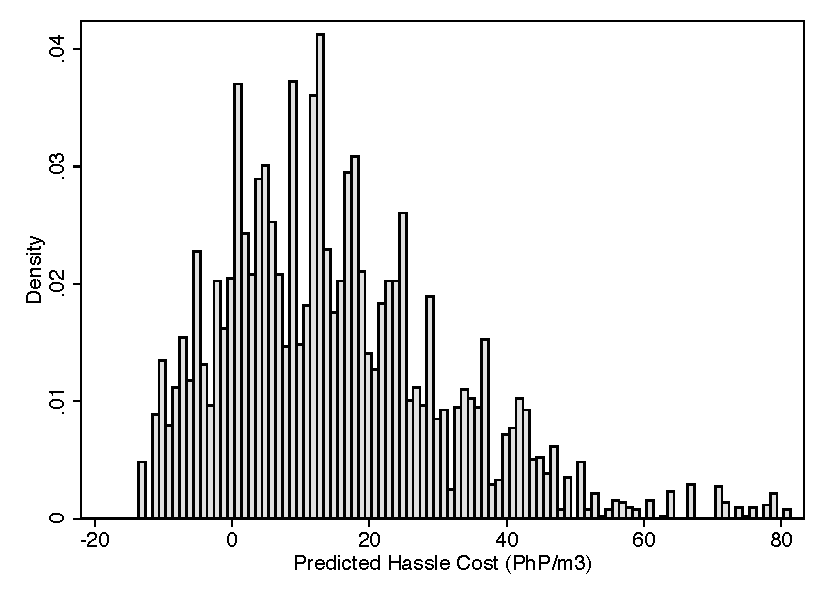
\includegraphics[scale=.7]{tables/hassle_cost_distribution.pdf} \\
%\vspace{cm}
\footnotesize{Excludes top and bottom 1\% outliers}
\end{table}

%Appendix~\ref{appendix:hasslecostbootstrap} includes more details on the bootstrapping procedure.

\subsection{Fixed Cost Estimation}\label{section:fixedcostestimation}

This section details how unobserved fixed costs of owning a connection are recovered from cross-sectional variation in water source choices.  The third step of the estimation uses the preference parameters recovered in Section~\ref{section:preferenceestimation} and hassle cost estimates from Section~\ref{section:hasslecostestimation} to simulate the initial water source choices for households.  By matching observed with predicted source choices, the estimation recovers the fixed costs of using a connection as well as prices associated with fetching from a vendor.  The fixed costs capture both one-time costs put into monthly terms --- connection fees, permitting with local governments, etc. --- as well as monthly costs --- service fees, plumbing maintenance, etc.  

The fixed cost estimation sample includes the random sample of 5,000 connections from the preference estimation.\footnote{This sample excludes connections used to estimate hassle costs since the majority of these connections use imputed demographics.}  I merge the estimation sample with the subsample of households using water from small-scale vendors drawn from the Census of Population and Housing 2010 as described in Section~\ref{section:data}.  Neighborhoods of potential sharing partners are limited to groups of three households, which is consistent with the vast majority of households forming sharing relationships of three households or less.  Within a three person neighborhood, households can share with a maximum of two other households. Assuming a limited neighborhood size and restricting households to only share within their neighborhoods both work to reduce sharing opportunities for households.  Since high fixed costs for new connections incentivize sharing, this approach may underestimate the true fixed costs faced by households.  

\subsubsection{Disaggregating Connection-Level Preferences to Household-Level Preferences}

In order to simulate these choices, I first need to recover household-level preferences from the connection-level preferences estimated in Section~\ref{section:preferenceestimation}.  Household price sensitivity, $\alpha_i$, can be inferred as a linear function of the vector of demographics specific to each household, $Z_i$, and estimates of $\alpha_C$.  Since fixed preferences $\hat{\gamma_C}$ are estimated non-parametrically at the connection-level, I specify a parametric method of splitting $\hat{\gamma_C}$ into $\gamma_i$ for all households using demographics, $Z_i$:
\begin{align*}
\hat{\gamma_C}  		   		& =  \sum_{i=1}^{S} ( \gamma_i - \alpha_i H_{i} ) \\
\big [ \hat{\gamma_C} - \sum_{i=1}^{S}  \alpha_i H_{i} \big ]		& =  \sum_{i=1}^{S}  (\lambda_{S} Z_i + \mu_{i})  
\end{align*}
$Z_i$ captures demographic characteristics specific to each household.  $\lambda_{S}$ are coefficients measuring the effect of these demographics on fixed preferences $\gamma_C$.  These coefficients are allowed to differ across connections serving different numbers of households, $S$ as well as whether household $i$ is an owner of the connection.  $\mu_{i}$ captures any residual variation that is unexplained by demographics.  In this case, $Z_i$ consists of household size since it is the only demographic measure reported separately for connection owners and other users.  I estimate a simple regression to recover estimates of $\lambda_{S}$, which provides predicted levels of $\gamma_i$ for each household.  Finally, this method needs to allocate any residual variation in preferences $\mu_{i}$ across the households.  Instead of either allocating $\mu_i$ entirely to the connection owner or splitting $\mu_{i}$ evenly across households, I allocate $M \mu_{i}$ to the owner and $\frac{(1-M)}{S-1} \mu_{i}$ to neighboring users where $M$ is the ratio of average connection-level preferences for single users, $\gamma_{S=1}$ to average connection-level preferences for shared connections $\gamma_{S>1}$.  This approach nests the assumption that connection owners are more likely than their sharing partners to resemble the water demand of single-users.  Another limitation is that the data only provide the total number of people using a connection for shared connections.  Therefore, in cases where three households use a connection, I assume that sharing people are allocated evenly between the two sharing households.
%%% , which is consistent with the discussion in Section~\ref{section:watersourcechoice}

\subsubsection{Imputing Preferences for Households using from Water Vendors}

Given the full set of household-level demand parameters for connected households, I then impute preferences for households using from vendors.  $\alpha_i$ can be computed simply from demographic measures, $Z_i$, for these households.  Since $\gamma_i$ is estimated non-parametrically for connected households, I use a regression with location, demographic variables, and their full set of interactions to impute preferences for households using from vendors:
\begin{align*}
\gamma_i = \beta_0 Z_i + \beta_1 L_i + \beta_2 Z_i L_i + \zeta_i
\end{align*}
$Z_i$ contains demographics while $L_i$ includes dummy variables for small census areas.  After recovering coefficients for the sample of connected households, I then compute predicted $\gamma_i$ for households using water from vendors.  This method requires the assumption that unobserved variation in preferences $\zeta_i$ is uncorrelated between connected households and households using from vendors.  This assumption may not hold if unobservable aspects of preferences drive some households to use from vendors.  Since vendors offer high marginal prices, this form of selection would likely lead the method to overestimate demand among households using from vendors.  

Disaggregating connection-level preferences as well as including households using from vendors combine to expand the sample from 6,363
 connections to  households.

\subsubsection{Simulation and Estimation}

With the full set of household preferences, the simulation routine first groups households into random sets of three neighbors with each of the 8 geographic regions.  The routine then orders households in the sequential game according to their utilities from using an individual connection.  This assumption captures the intuition that households who would have connected in the absence of any sharing are likely to be the first to take-up a new connection.  Random draws of the preference shocks, $\eta$ and $\epsilon$, are assigned to each household so that households can compute expected utilities over 5
months for all possible water source choices.  These shocks are sampled from a multivariate normal distribution taking into account the estimated correlation between sharing partners from Table~\ref{table:correstimates}.  
%\footnote{ Future versions will not condition on observed choices in this way, and instead sample households across sharing relationships. }

Households calculate payoffs following Section~\ref{section:watersourcechoice} given all potential choice sets.  Appendix~\ref{appendix:gametreefull} maps the full game tree with three players that is simulated in the estimation.  This sequential game is repeated 10
times to construct a set of draws to compute simulated moments.  The moments used in the estimation include the shares of households choosing different sources --- using an individual connection, using water from a neighbor, and using from a vendor --- as well as the covariance between each of these source choices and the fixed preference parameters for each household, $\gamma_i$.\footnote{I ensure that the estimation places heavier weight on matching the source-choice moments over the correlation moments because these correlations rely on possibly noisy measures of the preference parameters both due to incidental parameter issues in estimation as well as imputation for households using vended water. }  % Future versions will re-weight these moments given the boot-strapped variance-covariance matrix.

\begin{table}
\centering
\caption{Simulated Method of Moments Estimates}\label{table:smmestimates}
\begin{tabular}{lcc}
& Estimate & Standard Error \\
\hline
Fixed Cost per Connection (PhP/Month): $F$ &348.42&42.34\\
Fixed Cost for Vended Water (PhP/Month): $F_{V}$ &141.19&14.78\\
Price for Vended Water (PhP/m3): $P_{V}$ &39.80&2.54\\
Vendor Price Variance: $\sigma_{V}^2$  &8.20&0.67\\
\hline
\end{tabular}
\\
\vspace{.05cm}
\footnotesize{ Standard errors are bootstrapped at the connection level.  Total Households:  6,363
  }
\end{table}

Table~\ref{table:smmestimates} presents the estimation results, finding a total estimated monthly fixed cost of 348
PhP, which is around 50\% higher than the 225
PhP monthly fixed fee paid the provider.  This finding suggests that households face sizable barriers to connecting to the water network such as maintenance land tenure insecurity, or administrative costs.  This total fixed fee is also comparable to the total variable price paid to the provider each month in Table~\ref{descriptives}, suggesting that fixed costs compose almost half of the total costs of using piped water.  

The estimates also reveal a fixed cost for vendors equivalent to 141
PhP per month.  This likely captures fixed quality differences between vended water and other water sources.  The mean price for vended water of 40
PhP per cubic meter is close to the highest tariff price in Figure~\ref{figure:tariff}.  These estimates include a sizable variance term for the vendor price, which is consistent with the large variety of small-scale water sources that are collapsed into this measure, including primarily deep wells as well as tanker trucks and water refilling stations.  These sources may also be unevenly distributed throughout the city.

Since consumer surplus from using piped water is defined relative to using from a vendor, the magnitudes of the welfare calculations may be sensitive to the parameter estimates of the vendor option, particularly the marginal price, $p_v$.  As a simple out-of-sample test, I compare this estimate of $p_v$ to the implied $p_v$ from data on total water expenditures for vendor households using additional census data from a section of Manila.\footnote{The 2011 Community Based Monitoring System data covers over 70\% of households in Pasay City --- a large area with a population of 500,000 in downtown Manila --- and includes information on income (used to compute imputed income) as well as water source and monthly expenditures.}  In this data, households using from vendors report expenditures of 365 PhP/month while households using individual connections report expenditures of 470 PhP/month and households sharing connections report expenditures of 370 PhP/month.  Assuming that the vendor expenditures only reflect the marginal prices paid for water (excluding the fixed cost), I can express average expenditures, $E_v$, by multiplying average vendor demand by the vendor price, $E_v = (\gamma - \alpha p_v) p_v$.  Plugging in expenditures, $E_v =365$ PhP/$\text{m}^{3}$, average fixed preferences for vendors, $\gamma=33$, and price sensitivity, $\alpha=.62$, as well as solving the quadratic expression, I find that this level of expenditure is consistent with vendor prices of either 15.7 PhP/$\text{m}^{3}$ or 37.53 PhP/$\text{m}^{3}$.  The latter price matches closely to the estimated price of 37.16 PhP/$\text{m}^3$, providing additional support to the structural estimates.


\subsection{Out-of-Sample Test}\label{section:oostest}

To evaluate how well the model is able to match observed substitution patterns between water sources, I investigate reduced-form evidence from a connection-fee discount program since this variation is not used explicitly in any part of the estimation.  The fundamental assumption of the model is that the decision to share a water connection balances splitting the fixed fee among many households against facing marginal hassle costs in fetching water as well as free-rider costs in splitting the water bill.  Under this assumption, reducing the fixed fee would lead to substitution away from shared connections toward individual connections.  This section uses quasi-experimental variation in the connection-fee to test this assumption.

In 2009, the government regulator issued new regulations reducing the connection fee from 6,000 to 2,400 PhP for low-income areas partially in an effort to extend access and affordability to low-income households.  Under the assumption that households reside in Manila for 80 months and face negligible credit constraints, this discount lowered the monthly fixed fee faced by households by 45 PhP on average.  In the presence of credit constraints, this estimate can be interpreted as a lower bound on the policy's impact on the monthly fixed price faced by households.  Figure~\ref{figure:discountfirststage} indicates the share of new connections receiving discounted fees.  The sudden rise by 37percentage points coincides with the change in regulations and will be used to identify the timing of the discount policy.  A small fraction of households are observed to receive connection fee discounts prior to the program as part of other, smaller pro-poor strategies implemented by the water provider.

\begin{figure}
\centering
\caption{Share of New Connections Receiving a Discount}\label{figure:discountfirststage}
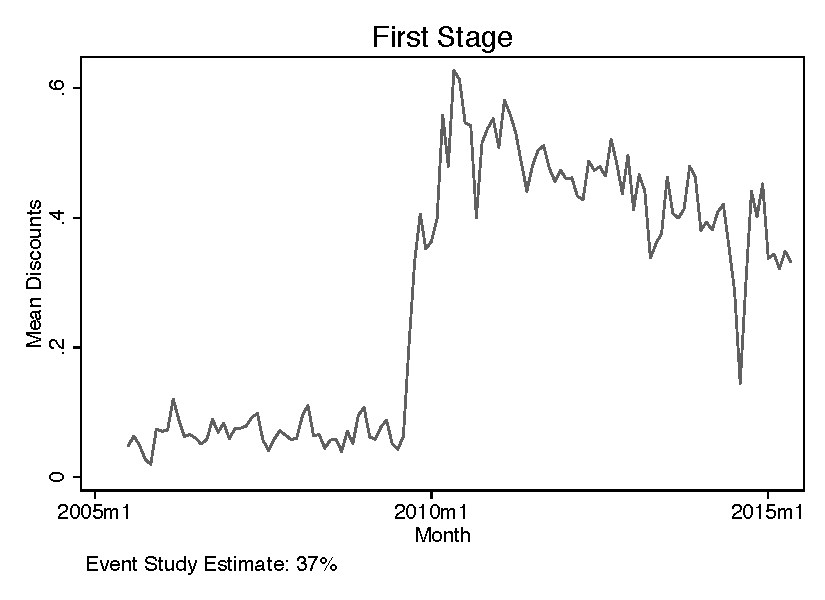
\includegraphics[scale=.7]{tables/diff_595_first_stage.pdf}
\end{figure}

Since the data do not identify precisely which local areas or specific households were eligible for the discount, additional assumptions are necessary to measure eligibility.  First, I define treated areas as any meter reading unit that receives at least one discounted connection over the full duration while control areas include any meter reading units that never receive discounts.  Meter reading units (MRUs) are common geographical designations used by the water provider and include between 100 and 500 meters.  There are 3,757 MRUs in the service area.  I include only MRUs that were established long prior to the discount fee program to ensure that these areas are likely to be at saturation in terms of water connections prior to the program.  Second, to identify the share of households in treated areas that were eligible, I conceptually divide new connections into two groups --- (1) households substituting away from shared connections or water vendors in response to the program and (2) new households migrating to the city.  I then measure eligibility as the share of new migrants receiving discounted connections fees after the policy.

This approach requires the following assumptions:
\begin{enumerate}
	\item Before the discount program, households that have already moved to the city have reached an equilibrium at the current prices; therefore, all new full-price connections in the pre-period are driven by migration to the city.  This assumption is consistent with the large fixed costs incurred in setting up a new connection.
	\item The rate of migration is unaffected by the policy, which is supported by the stable rate of new connections for untreated areas in Figure~\ref{figure:discountreducedform} below.  
	\item After the discount policy is implemented, all new migrant households that are eligible take up the discounted connections.
	\item Rates of eligibility are similar across migrant and non-migrant groups.
\end{enumerate}
Under these assumptions, I compute the impact of the policy on new full-price connections in the treated areas and interpret any reduction in the rate of new full-price connections as driven by new migrants receiving discounted connections.  I estimate the following simple difference-in-differences equation across all treated and untreated Meter Reading Units, $m$, and months, $t$, pre and post policy implementation:
\begin{align*}
\text{New Full-Price Connections}_{t,m} &= \beta_1 \text{Post X Treated}_{t,m} + \beta_2 \text{Post}_{t,m} + \beta_3 \text{Treated}_{t,m} + \epsilon_{t,m}
\end{align*}
Table~\ref{table:difffullpriced} presents the results from this estimation.\footnote{These results do not exactly match reduced-form results from Table~\ref{table:diffdiscountreducedform} because the data only have information on the price per connection for about 80\% of new connections.}  Adding the coefficients in Table~\ref{table:difffullpriced} shows that in the absence of the policy, treated areas were expected to have added 0.64new full-price connections each month; yet, as a result of the policy, these areas actually experienced 0.46new full-price connections with the remaining households receiving discounted connections.  This discrepancy implies that 28\unskip\% of households were eligible for the program.

\begin{table}
\centering
\caption{Difference-in-Differences Estimate for Full Priced Connections}\label{table:difffullpriced}
\begin{tabular}{lc} \hline
 & (1) \\
VARIABLES & Diff-in-Diff Estimate \\ \hline
 &  \\
Post X Treated & -0.184*** \\
 & (0.0168) \\
Post & 0.205*** \\
 & (0.00976) \\
Treated & 0.343*** \\
 & (0.0156) \\
Constant & 0.0901*** \\
 & (0.00677) \\
 &  \\
Observations & 382,462 \\
R-squared & 0.004 \\
 Avg. New Conn. & .39 \\ \hline
\multicolumn{2}{c}{ Robust standard errors in parentheses} \\
\multicolumn{2}{c}{ *** p$<$0.01, ** p$<$0.05, * p$<$0.1} \\
\multicolumn{2}{c}{ Clustered at the MRU Level: 3,757 MRUs} \\
\end{tabular}

\end{table}

I next examine the reduced-form impacts of the policy using the following event-study regression equation, which computes the average number of new connections in bi-monthly intervals relative to the discount fee program for both treated and untreated areas:
\begin{align*}
\text{New Connections}_{t,m} &= \sum_{r=0}^{T} \beta^{\text{Treated}}_{r} \mathbbm{1} \{t=r\} + \sum_{r=0}^{T} \beta^{\text{Untreated}}_{r} \mathbbm{1} \{t=r\}  +  \theta_{m} + \epsilon_{t,m} \\
t &= \text{2 Month Intervals}\\
m &= \text{Meter Reading Unit}
\end{align*}
Figure~\ref{figure:discountreducedform} provides the graphical estimates from this equation.  The untreated group on the left-hand side exhibits a very stable trend in new connections with no changes relative to the discount program.  This finding is consistent with steady population growth generating a constant rise in the total number of connections.

The treated group on the right-hand side shows a relatively stable pre-trend interrupted by a substantial increase in the number of connections just following the discount program implementation.  This increase lasts for a couple years before returning to pre-program levels.  These trends provide evidence that households who are sharing water or purchasing from vendors are gradually learning about the price change and choosing to purchase their own connections.  After a couple years, this additional demand for connections has been satisfied, letting migration take over as the sole driver of new connections.
\begin{figure}
\centering
\caption{Reduced Form: Connection Fee Discount}\label{figure:discountreducedform}
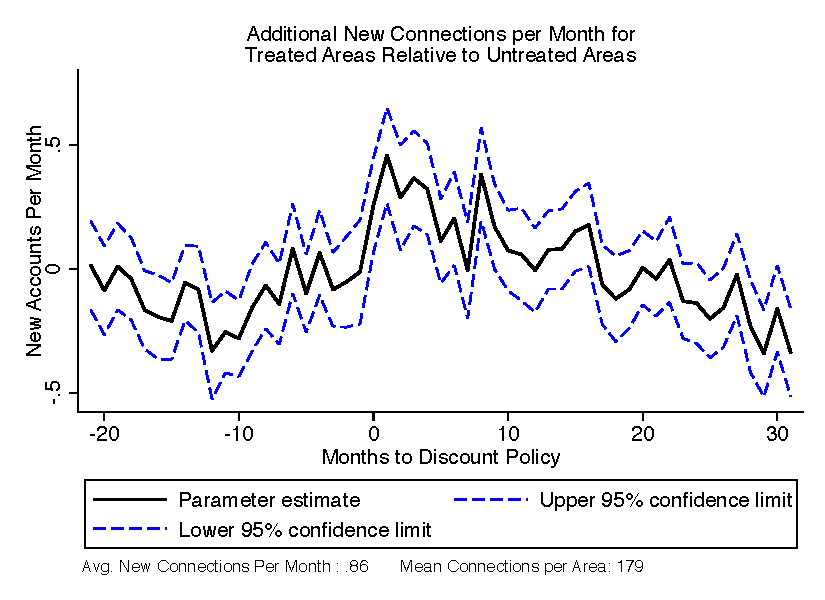
\includegraphics[scale=.8]{tables/diff_595.pdf}
%\includegraphics[scale=.57]{tables/diff_595_treated.pdf}
\end{figure}

\begin{table}
\centering
\caption{Difference-in-Differences Estimate}\label{table:diffdiscountreducedform}
\begin{tabular}{lc} \hline
 & (1) \\
VARIABLES & Diff-in-Diff Estimate \\ \hline
 &  \\
Post X Treated & 0.127*** \\
 & (0.0215) \\
Post & 0.0163 \\
 & (0.0122) \\
Constant & 0.794*** \\
 & (0.00855) \\
 &  \\
Observations & 382,462 \\
R-squared & 0.062 \\
Avg. New Conn. & .86 \\
 Area FE & Yes \\ \hline
\multicolumn{2}{c}{ Robust standard errors in parentheses} \\
\multicolumn{2}{c}{ *** p$<$0.01, ** p$<$0.05, * p$<$0.1} \\
\multicolumn{2}{c}{ Clustered at the MRU Level: 3,757 MRUs} \\
\end{tabular}

\end{table}

A simple difference-in-differences estimate provided by Table~\ref{table:diffdiscountreducedform} calculates an increase of 0.13new connections per month for the treated areas on a base average of 0.79new connections per month.  Aggregated over the full 69months of the program, this program led to a total of 8.74new connections per Meter Reading Unit.  Given that the average Meter Reading Unit has 179connections over the full time period, this program generated about a 3.5\unskip\% increase in the number of new connections.  

To compare results from this policy to counterfactual estimates from the model, I now convert the change in number of connections induced by the policy to a shift from shared and vendor connections to individual connections.  Given that 14\unskip\% of connections serve two households and 10\unskip\% of connections serve three or more households, and 5\% of households access water from vendors, then 179connections per Meter Reading Unit are calculated to serve an average population of around 250households.  This policy results in a 3.5percentage point increase in the share of households owning a connection, which can be directly compared to predictions from the counterfactual exercise.

In order to relate the quasi-experimental results from the policy to the model outputs, I simulate the impacts of the connection-fee discount policy by (1) randomly selecting 28\unskip\% of households, (2) lowering the fixed fee by 45 PhP for these households, and (3) recomputing their water source choices.  As a result of this policy, the share of households owning a water connection is calculated to rise by 1.34percentage points.  This finding is smaller, but comparable to the reduced form results indicating a 3.5percentage point increase.  There may be many reasons that the counterfactual results lag behind the reduced-form estimates.  First, the assumptions used to amortize the connection fee discount into monthly terms  may work to understate the impact of the discount, especially in cases where households face credit-constraints in funding large, lump-sum connection fees.  Second, in practice, the discount policy targeted a low-income segment of the population, which may have different substitution patterns across water sources.  

Despite these caveats, the fact that the reduced-form and model-based estimates are similar in magnitude lends support to the counterfactual exercises in Section~\ref{section:counterfactualexercises}.  Table~\ref{table:oosestimates} calculates the impacts of this connection fee discount on water source choices as well as consumer welfare.  Consumer welfare is computed as the difference between current utility and the utility that each household would receive from using vended water.  Since utility is assumed to be quasi-linear, consumer welfare is reported in PhP/month.  Lowering the fixed fee leads to substitution away from both vendor and neighbor water sources, which improves consumer welfare especially for the bottom 50\unskip\% of users.

\begin{table}
\centering
\caption{Connection Fee Discount: Out-of-Sample Test Results}\label{table:oosestimates}
\begin{tabular}{lcc}
%\hline
& Current &  Discount \\
\hline
%\hline
Fixed Fee (PhP) & 225 &180\\
Source Vendor & 0.044 & 0.039 \\
Source Neighbor &0.243 & 0.235 \\
 Surplus (PhP)  &143.0&153.1 \\
 Surplus: Low Users (PhP)  &76.4&84.0 \\
\hline
\end{tabular}
 \\ 
Consumer surplus is measured in PhP/month.
\end{table}


\section{Counterfactual Exercises}\label{section:counterfactualexercises}

This section reconstructs the economic problem faced by the regulator in order to investigate how alternative pricing policies might impact welfare.  I consider the government regulator's maximization problem given by equation (\ref{equation:regulator}) where the regulator chooses a fixed fee, $Fee$ and a price schedule, $P$, to maximize consumer surplus while covering the costs of production (holding profits equal to zero).  Consumer welfare is defined as the expected sum of all households' utilities subject to welfare weights, $\delta_i$, for different subpopulations, which capture any preferences the regulator may have towards redistribution.  The counterfactual exercises consider two sets of these preferences: (1) the regulator weights all utilities equally and (2) the regulator only considers utility for the bottom 50th percentile of water demand, summarized by the fixed water preferences $\gamma$ for each household.  Giving preference to low-demand households intends to capture dual policy goals of ensuring access as well as minimum monthly usage for all households.  Since low-demand households are also often low-income households, this preference also provides a proxy for standard preferences toward redistribution.\footnote{Using income directly is less informative due to noise in the imputation process, especially for households that are sharing with their neighbors.}  Similarly, this approach may capture efficiency gains if connecting low-users produces positive health externalities (\cite{galiani2005water,gamper2010impact}).  For ease of exposition, the utility function below nests the water source choices of each household.
\begin{align}
\begin{split}
max_{Fee,p_{L},p_{H}} &\hspace{.4cm} E\text{\LARGE [} \sum_{i=1}^{N} \delta_i U_{i}(Fee,p_{L},p_{H}) \text{\LARGE ]} \\
s.t. \hspace{.5cm} & \text{Total Connections} \times \big[ Fee - \text{Installation/Service Costs} \big] + \\
              & \text{Total Water} \times \big[ \text{Revenue per Unit}(p_{L},p_{H})  - \text{Marginal Cost}  \big] \\
      & \hspace{5.5cm} \geq \text{Capital Costs}
\end{split}
\label{equation:regulator}
\end{align}
The budget constraint ensures that the fixed monthly fee, $Fee$, paid to the company for each connection as well as the revenue earned for each unit of water consumption (given the non-linear pricing scheme) outweighs the costs of servicing each connection, the marginal costs of providing a cubic meter of water, as well as any capital costs associated with the pipe-network, pumping stations, and dam maintenance.  The water provider calculates that their marginal costs are equal to 5 PhP per $\text{m}^{3}$ and that the fixed fee exactly covers any installation/service costs.  To determine the capital costs, I subtract the total marginal and services costs from the total revenue earned by the company, assigning the remainder to capital costs.  Capital costs include maintaining the pipes, pumping stations, and billing infrastructure.  This calculation provides a close approximation to the Capital Expenditures regulatory structure implemented in this context, which exactly compensates the water provider for its costs through increases in the tariff.\footnote{This paper abstracts away from any principal agent problems between the company and the regulator by assuming that the regulator has perfect information over the firm's capital investments and operating costs (\cite{laffont1993theory}).}  This regulatory problem forms the basis for evaluating the following counterfactual policies.  All counterfactual policies evaluated below hold firm profits equal to zero.


\subsection{Compensated Fixed Fee Discount}

I first examine a counterfactual policy where the regulator discounts the upfront fee while increasing the tariff to remain revenue neutral.  By discounting the fixed fee by 45PhP, this policy mimics the policy implemented by the water provider; however, while the provider's discount decreased overall revenue, this policy imposes the necessary tariff increase to fund the lower fixed fee.  This counterfactual also echoes recent recommendations from policymakers and researchers including the World Bank who have strongly advocated for lower connection fees as a way of extending access to piped water among the poor (\cite{wsup,komives2005water,jimenez2014factors,kayaga2007costs,mcintosh2003asian}).  Figure~\ref{figure:discounttariff} indicates the current tariff and the compensated tariff, which is shifted upwards by 9.73PhP/$\text{m}^{3}$ to maintain revenue neutrality.  

\begin{figure}
\centering
\caption{Tariff Shift from Connection Fee Discount}\label{figure:discounttariff}
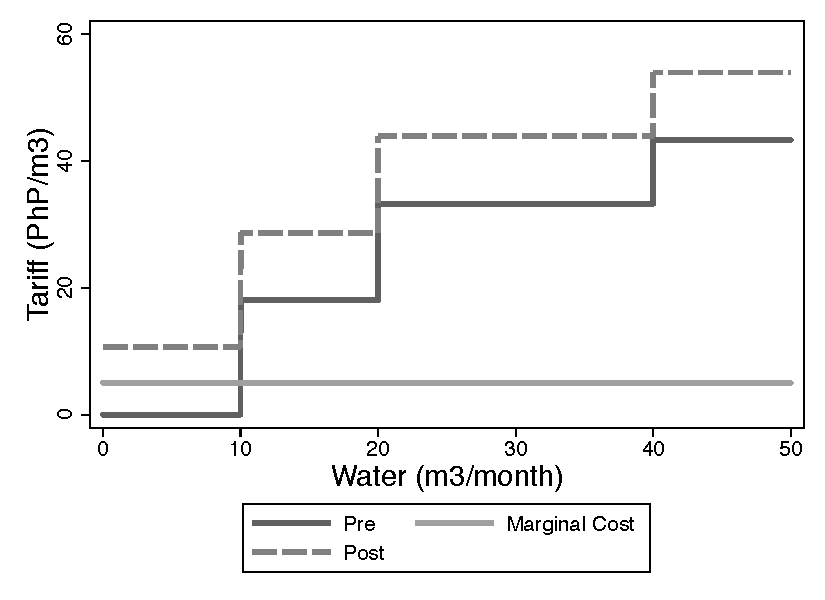
\includegraphics[scale=.7]{tables/discount_tariff_groups.pdf}
\end{figure}


Table~\ref{table:fixedfeediscount} summarizes the impacts of this change on source choices and consumer welfare measured in terms of the difference between current utility and utility from using the outside vendor option as in Section~\ref{section:oostest}.  The decrease in the fixed fee and increase in the tariff both act to decrease the incentives for sharing a connection and leading to a drop of 0.00percentage points in households using water from their neighbors.  The third row indicates even greater substitution toward water vendors of around 1.25percentage points in response to the higher tariff.  These effects combine to reduce average consumer surplus by 21.5PhP per month, which is over half of the initial fixed fee discount of 45PhP.  This decline translates into a 0.31percent loss of monthly household income.  Households in the bottom 50\unskip th percentile of water users also experience lower consumer surplus although the magnitude is much less, amounting to 0.03percent of monthly household income.  Taken together, these results suggest that connection fee discount policies in this context can have unintended distributional consequences by reducing both access to piped water and welfare for the intended beneficiaries. %\footnote{Consumer surplus is measured relative to utility from using vended water.}  
\begin{table}
	\centering
	\caption{Fixed Fee Discount Counterfactual}\label{table:fixedfeediscount}
	\begin{tabular}{lcc}
\hline
& Current & Discount \\
\hline
\hline
Fixed Fee (PhP/month) &381&336\\
Source Vendor &3.7\% &15.4\% \\
Source Neighbor &25.1\% &26.8\% \\
 Surplus  &218.6&105.2 \\
 Surplus: Low Users  &89.7&45.3 \\
\hline
\end{tabular}
 \\
	\footnotesize{Low Users include the bottom 50\% of water users. \\
	Surplus is measured in terms of PhPd/month.}
\end{table}

\subsection{Characterizing Optimal Tariff Schedules}

This section considers the welfare impacts of six tariff structures in order to inform water regulators who face a variety of institutional settings and redistributional priorities: while some regulators may be restricted to simple two-part tariffs, others can allow for complex, non-linear price schedules as in Manila (\cite{hoque2013state}).  Similarly, while encouraging efficient use, many developing countries also include distributional motivations for their tariff structures such as ensuring all households reach a certain minimum level of usage (\cite{szabo2015value}).

As a benchmark, this exercise first examines a First-Best tariff informed by the industrial organization literature where (1) the marginal price per unit of water equals the marginal cost of production, (2) every household pays a fixed fee just equal to costs of installing and maintaining a connection, and (3) the regulator is able to perfectly price discriminate according to household demand, extracting additional transfers from households to exactly fund the fixed capital costs (\cite{auerbach1978two,oi1971disneyland}).  Without sharing, this tariff follows economic theory to maximize efficiency.  I then compare how the current tariff in Manila performs relative to this First-Best tariff structure.
%Additionally in this case, I assume that the regulator can use these costless transfers to reallocate surplus from high users to low users in order to achieve distributional goals as well.  

The next tariff imposes restrictions on the regulator by only allowing for a simple two-part tariff with a monthly fixed component and a single variable component.  First, I look for the two-part tariff that maximizes overall consumer surplus.  Second, I define a social two-part tariff, which maximizes surplus for low users and provides a means of summarizing regulator preferences toward redistribution or ensuring basic levels of access.  Low users are classified as households with fixed preferences for water usage, $\gamma$, below the average level.  Since households exhibit little heterogeneity in their price sensitivities, $\alpha$, this approach provides a simple method to summarize water demand across the population.  
%An alternative approach may be to examine welfare impacts by household incomes; however, the data only allow for noisy imputations of income, which may mask larger distributional effects.  Additionally, placing extra welfare weight on smaller users captures the spirit of recent goals by policymakers to ensure a basic right to water.  

Finally, I calculate optimal three-part tariffs, which include a fixed fee and separate marginal prices for consumption below and above a 20 cubic meter threshold.  This structure more closely mirrors the current tariff implemented in Manila.\footnote{I calculate optimal tariffs for a 5\% subset of the sample since non-linear budget constraints make this process computationally expensive.  Preliminary tests suggest that the results are robust to this sampling technique.}

\subsubsection{Optimal Tariffs Without Sharing}\label{section:optimaltariffswithoutsharing}

This section computes optimal tariffs when sharing is prohibitively expensive.  This counterfactual setting without sharing allows me to (1) verify optimal tariff designs from the economics literature without sharing and (2) examine the extent to which these tariff designs resemble current pricing policies in Manila.  When households are unable to share, the provider raises less revenue at the current tariff.  Therefore, I recalculate a lower level of capital costs according to revenue generated by imposing the current tariff without sharing.  This procedure allows for direct welfare comparisons between the current tariff and counterfactual tariffs; however, because of this procedure, the magnitudes of the results in this section are not directly comparable to counterfactuals with sharing in Section~\ref{section:optimaltariffswithsharing}.

Figure~\ref{figure:optimaltariffnosharing} provides the optimal tariffs without sharing, and Table~\ref{table:optimaltariffnosharing} includes the corresponding monthly fixed fees as well as the impacts of these tariff structures on the share of households using vendors and using neighboring connections.  The last two rows include consumer surplus measures for the average household as well as the bottom 50\% of users.  Since producer surplus is always held to be zero in these exercises, these consumer surplus measures fully capture welfare.  For ease of comparison, Table~\ref{table:optimaltariffnosharing} also includes the average tariff level in the second row.

\begin{figure}
\centering
\caption{Optimal Tariffs Without Sharing}\label{figure:optimaltariffnosharing}
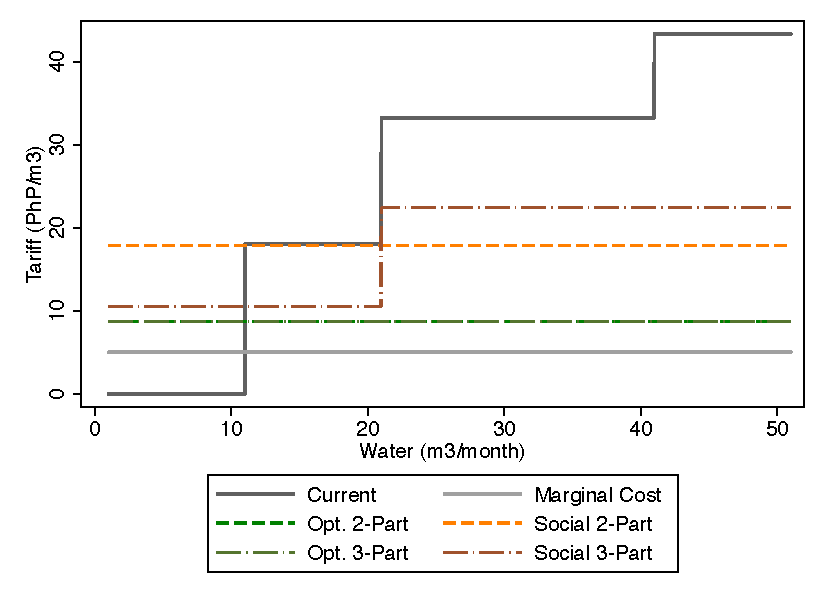
\includegraphics{tables/no_shr_tariff_groups.pdf}  
\end{figure}

The First-Best tariff schedule produces the highest level of consumer surplus reaching 385.1PhP/month or 1.64\unskip\% of household income.  This tariff also produces the minimum share of households using vended water at 21\unskip\%.  With costless transfers, the regulator could theoretically reallocate all surplus to the lowest users providing an upper bound on redistribution through pricing at almost double the average surplus.  

Relative to the First-Best, implementing the current tariff in this context without sharing reduces average surplus dramatically and increases the share of households using vended water by raising the average marginal price.  The optimal two-part tariff in column three features a higher fixed fee affording a lower marginal price at all consumption levels.  Compared to the current tariff, the optimal two-part tariff brings consumer surplus up to 94\unskip\% of the First-Best surplus.  These welfare gains are primarily driven by increased consumption for large users since surplus for low-users is cut in half and the share of households connected to the network declines substantially.

\begin{table}
\centering
\caption{Optimal Tariffs Without Sharing}\label{table:optimaltariffnosharing}
\resizebox{\textwidth}{!}{%
\begin{tabular}{lcccccc}
  & First-Best & Current & 2-Part  & 2-Part Social  & 3-Part & 3-Part Social \\
\hline
\hline
Fixed Fee (PhP/month) &225&225&290&31&293&108\\
Avg. Tariff (PhP/m3) &5.0&22.5&9.0&17.7&8.9&17.6\\
Source Vendor &21\% &25\% &33\% &19\% &33\% &21\%\\
Source Neighbor &0\% &0\% &0\% &0\% &0\% &0\%\\
Surplus &324.6&124.1&310.5&265.6&310.6&239.8\\
Surplus: Low Users &564.5&48.5&35.5&66.8&36.3&75.6\\
Consumption (m3/month) &33.8&17.3&28.7&24.9&28.6&23.0\\
\hline
\end{tabular}

}	\\
\footnotesize{$\text{ }^{*}$ The First-Best fee does not include individual transfers imposed by the regulator. \\  Social tariffs place all welfare weight on the bottom 50\% of water users. \\ Surplus is measured in terms of PhP/month.}

\end{table}

The optimal social tariff in column four attempts to offset these welfare losses for low users by reducing the fixed fee just below zero and doubling the marginal price.  The low fees incentivize small users to connect to the network, reducing the share using from vendors to the First-Best levels.  Average surplus declines since high marginal prices reduce consumption for large users; however, surplus for low users more than doubles.  This result points to the attractiveness of using non-linear pricing to achieve normative goals of redistribution when shared connections are infeasible.

By adding an extra segment to the tariff schedule, the fifth column tests the extent to which more complex linear tariffs can improve efficiency.  Figure~\ref{figure:optimaltariffnosharing} graphs this three-part tariff relative to the current tariff.  The shape of the optimal three-part tariff resembles the current tariff with a low first segment followed by a higher second segment (although the optimal three-part tariff maximizes total surplus while the current tariff is motivated by distributional concerns).  The intuition for this finding is that a low first price segment combined with a high fixed fee provides an additional mechanism for the regulator to price discriminate on the extensive margin; under this pricing regime, only relatively large users connect and their high usage allows the regulator to further lower prices (since the marginal price well exceeds marginal cost).  Despite this attempt to improve welfare, surplus changes are negligible.  

The social three-part tariff in column six has slightly more success in redistributing surplus by using an additional tariff block extract greater revenue from large users and improve reallocation to low users.  Relative to the social two-part tariff, the social three-part tariff achieves this goal by offsetting a lower first price segment with a higher second price segment.  


\subsubsection{Optimal Tariffs With Sharing}\label{section:optimaltariffswithsharing}

This section calculates the optimal tariff structure in the current environment in Manila (when sharing is possible subject to the estimated hassle costs).  Figure~\ref{figure:optimaltariffsharing} plots the marginal prices associated with each counterfactual tariff.  Table~\ref{table:optimaltariffsharing} computes the impacts of these tariffs on source choices as well as welfare.  Comparing columns two and three of Table~\ref{table:optimaltariffsharing}, I find large welfare improvements on the order of 84\unskip\% of consumer surplus or 1.1\unskip\% of household income from shifting from the current tariff schedule to an optimal two-part tariff schedule.  These gains are mainly enjoyed by large users benefiting from a lower marginal price relative to the current tariff.  At the same time, flattening the tariff greatly reduces the implicit ``tax'' on shared connections, allowing small demand households to also benefit from lower marginal prices through their neighbors' connections.  These lower marginal prices almost compensate for the higher hassle and free-rider costs facing low-demand households, leaving surplus for these households unchanged.
%zooming in on tariffs below 20 PhP/$\text{m}^{3}$ in order to highlight distinctions between the two-part and three-part tariffs.  
\begin{figure}
\centering
\caption{Optimal Tariffs With Sharing}\label{figure:optimaltariffsharing}
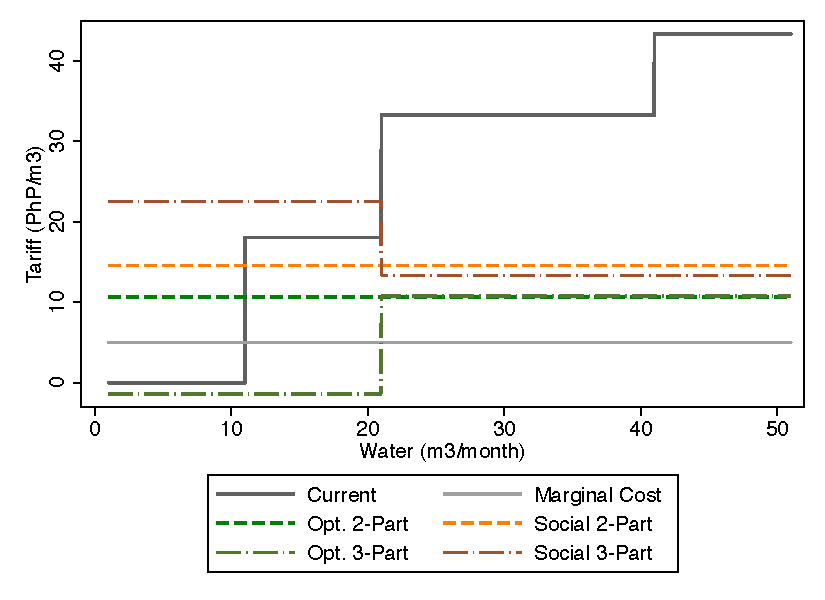
\includegraphics{tables/shr_tariff_groups.pdf}
\end{figure}

The optimal fixed fee lies below the current fixed fee, which is priced at the cost of installing and maintaining a connection.  Since households incur hassle costs and free-rider distortions from splitting the bill in sharing connections, pricing below cost allows the regulator to encourage households to substitute away from shared connections toward individual connections and avoid these hassle costs at the margin.  By subsidizing individual connections, the two-part tariff in column three performs very close to the First-Best tariff in terms of average consumer surplus.  

\begin{table}
\centering
\caption{Optimal Tariffs With Sharing}\label{table:optimaltariffsharing}
\resizebox{\textwidth}{!}{%
\begin{tabular}{lcccccc}
  & First-Best & Current & 2-Part  & 2-Part Social  & 3-Part & 3-Part Social \\
\hline
%\hline
Fixed Fee (PhP/month) &225&225&259&108&490&-12\\
Avg. Tariff (PhP/m3) &5.0&22.5&10.3&13.6&4.4&17.0\\
Source Vendor &1\% &4\% &1\% &0\% &1\% &0\%\\
Source Neighbor &39\% &25\% &44\% &37\% &44\% &35\%\\
Surplus &372.1&142.5&365.4&357.9&367.2&349.2\\
Surplus: Low Users &741.9&78.5&119.3&123.7&121.4&123.8\\
Consumption (m3/month) &35.7&17.9&31.9&30.6&32.0&30.2\\
\hline
\end{tabular}

}
\footnotesize{$\text{ }^{*}$ The First-Best fee does not include individual transfers imposed by the regulator. \\  Social tariffs place all welfare weight on the bottom 50\% of water users. \\ Surplus is measured in terms of PhP/month.}
\end{table}

Moving to a social two-part tariff in column four, I find that maximizing welfare for low users counterintuitively involves increasing the fixed fee in order to subsidize a very low marginal price.  This tariff maximizes the share of households using from neighbors while also driving a significant share of households toward water vendors.  Since low-users are able to split the fixed fee with their sharing partner, they can enjoy greater consumption at the low marginal price.  Despite this relatively extreme pricing schedule, surplus for low users only increases by 4.4PhP/month while average surplus declines by -43.0PhP/month.  While manipulating the two-part tariff proved to be an effective redistributive strategy without sharing in Section~\ref{section:optimaltariffswithoutsharing}, this finding suggests that informal sharing networks act to constrain the effectiveness of non-linear pricing in redistributing surplus.  

An optimal three-part tariff with sharing in column five follows the same pattern as in the case without sharing: moving to an increasing tariff structure selects for high-usage connections, which provide greater revenue to cover the fixed costs.  As before, this tariff produces negligible changes in welfare.  Figure~\ref{figure:optimaltariffsharing} indicates an optimal three-part tariff with an almost zero first price segment followed by a much higher second price segment, which again broadly aligns with the current tariff structure.  This tariff structure supports the ``life-line'' tariff as a way of efficiently maximizing surplus (rather than achieving distributional goals).  Column six (along with Figure~\ref{figure:optimaltariffsharing}) finds no difference in the optimal social two and three part tariffs.  This result points to the extent to which sharing networks constrain the ability of cities to achieve redistribution through complex, non-linear pricing strategies.


\subsubsection{Optimal Two-Part Tariffs and Sharing Hassle Costs}

To investigate mechanisms driving these optimal pricing schedules, this section considers how the optimal two-part tariff varies continuously with counterfactual levels of the hassle cost, $p_h$.  I follow the same routine as in Sections~\ref{section:optimaltariffswithoutsharing} and \ref{section:optimaltariffswithsharing} by (1) calculating total revenue raised under the current tariff (in Figure~\ref{figure:tariff}) given the counterfactual hassle cost, (2) recalculating the implied capital costs from total revenue under this hassle cost, and (3) determining the optimal two-part tariff maximizing total consumer surplus while just covering costs.\footnote{As the hassle cost rises, the current tariff raises less revenue, lowering the capital costs.  The patterns below are robust to instead holding the capital costs fixed while increasing the hassle costs.}

Figure~\ref{figure:tptshrcosts} plots the optimal marginal price, fixed fee, and share of the population choosing each water source as a function of the hassle cost.  The vertical gray lines show the estimated hassle cost of 15.14 from Section~\ref{section:hasslecostestimation}.  When hassle costs are very low, the regulator chooses a relatively high marginal price and low fixed fee.  This equilibrium maximizes sharing so that one third of households purchase connections and each share their connection with two neighbors.  The high marginal price serves as an way to mitigate overconsumption from free-riding on these shared connections: when three households share a tap, they respond to one third of the marginal price through spitting the bill.  Therefore, setting a price around 13 PhP/$\text{m}^3$ ensures that households actually respond close to the marginal cost of 5 PhP/$\text{m}^3$.  This high marginal price also raises greater revenue allowing the regulator to lower the fixed fee.  As the hassle cost increases to 5 PhP/$\text{m}^3$, the optimal marginal price decreases as more households substitute away from sharing arrangements.  This substitution reduces the extent of free-rider distortions, driving the marginal price closer to the marginal cost.

As the hassle cost increases from 5 PhP/$\text{m}^3$ to around 17 PhP/$\text{m}^3$, it becomes optimal for the regulator to increase the marginal price as a way of taxing shared connections and subsidizing individual connections.  In this range, households are not able to internalize the extent to which costly sharing relationships reduce their own contributions to the capital costs.  Therefore, a high marginal price serves as an additional disincentive for sharing.

Above 17 PhP/$\text{m}^3$, the hassle cost becomes large enough to disincentivize sharing on the margin, allowing the regulator to begin lowering the marginal price again.  Yet, at these high levels of hassle cost, some households begin substituting toward vended water, providing a new incentive for subsidizing access by keeping prices above the marginal cost (consistent with theoretical work by \cite{auerbach1978two}).  The slow decline in marginal price over this range helps to offset the increasing hassle cost, reducing the rate of substitution away from shared connections.  From a distributional perspective, I find that a hassle cost of around 18 PhP/$\text{m}^3$ represents a threshold where the bottom 50\% of users transition from preferring a very high fixed fee as in Section~\ref{section:optimaltariffswithsharing} to preferring fixed fee subsidies as in Section~\ref{section:optimaltariffswithoutsharing}.  

This exercise demonstrates how the presence of water sharing can have additional implications for optimal water pricing.  Free-rider behavior among sharing households creates an incentive for the regulator to maintain high marginal prices, and large hassle costs similarly motivate high marginal prices as an efficient tax on shared connections.


\begin{figure}
\caption{Two-Part Tariffs and Sharing Hassle Costs}\label{figure:tptshrcosts}
\begin{center}
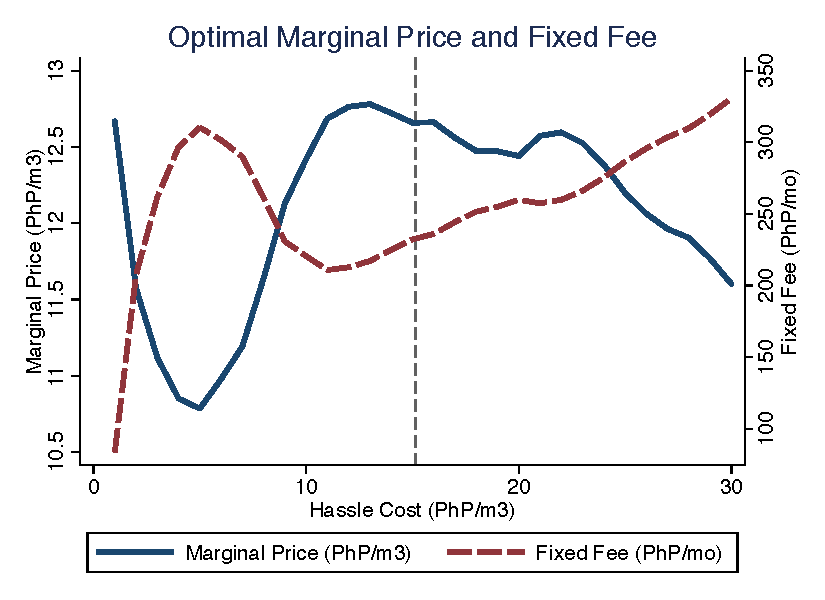
\includegraphics[scale=.55,valign=t]{tables/tpt_full_graph_prices.pdf}
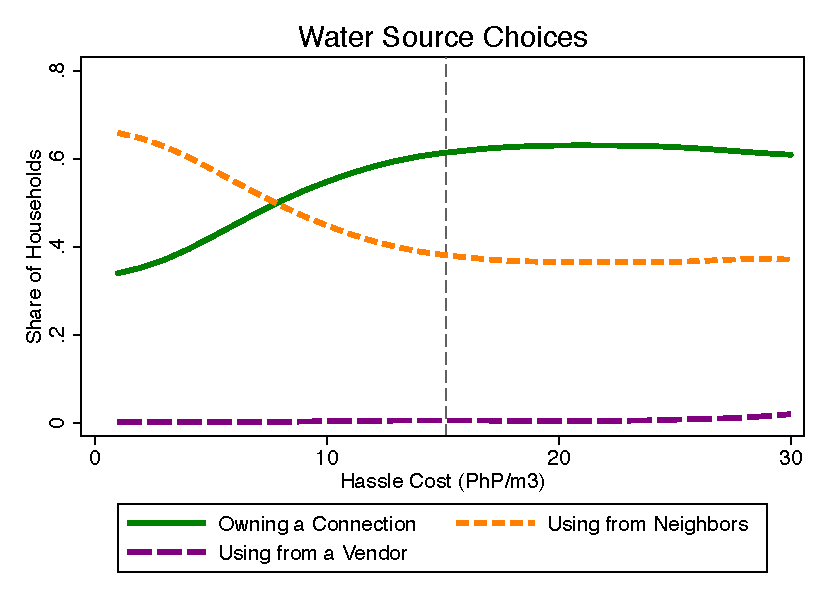
\includegraphics[scale=.58,valign=t]{tables/tpt_full_graph_shares.pdf}\\
{\footnotesize The vertical gray lines show the estimated hassle cost of 15.14 PhP/$\text{m}^3$ from Section~\ref{section:hasslecostestimation}.}
% \\ Marginal prices and fixed fees are smoothed with a moving average.}
\end{center}
\end{figure}


\section{Conclusion}\label{section:conclusion}

% didnt show this yet.... This paper finds that incorporating a model of informal sharing networks into a standard regulatory problem produces substantively different policy recommendations with potentially large welfare implications. 

This paper demonstrates that pricing policies intended to increase water access especially among the poor can have unintended consequences when low-income households can simply access the piped water network through their neighbors.  The counterfactual exercise finds that a simple two-part tariff structure outperforms the increasing block tariff currently implemented in Manila in terms of overall access to water and total welfare while leaving welfare among low-users unchanged.  In this counterfactual, high fixed costs of accessing an individual connection allow for sharing networks to play an important role in extending water access despite sizable hassle costs.  I also find that complex non-linear price schedules are largely ineffective in terms of achieving both efficiency and equity goals when sharing networks are readily available.  

Taken together, these results suggest that households may act as efficient subcontractors in redistributing water to their neighbors.  Instead of sending trained engineers to install and maintain connections in dense neighborhoods, providers can instead rely on informal networks to extend water distribution.  From this perspective, cities may benefit from considering how prices not only might encourage access and redistribute consumer surplus, but also may affect the endogenous formation of water sharing networks.  For example, price discriminating according to neighborhood income instead of by level of monthly usage may achieve similar goals of redistribution without distorting sharing networks.  While this policy may not be appropriate in Manila since neighborhoods are often very heterogeneous in income, this approach may work well in other contexts where neighborhoods are more segregated, such as in Colombia where electricity rates vary according to the social category of each neighborhood (\cite{mcrae2014infrastructure}).  

Since sharing networks constrain the menu of pricing policies available to policymakers, cities may benefit from considering a broader range of policies to improve welfare from water use.  For example, cities may be able to lower the frictions associated with these sharing networks by providing technical resources for managing plumbing networks or distributing extra water meters to assist households in accurately splitting the bill.  The empirical results also confirm previous findings that substantial barriers exist for households to connect to the network (\cite{devoto2012happiness}).  Cities may be able to similarly achieve substantial welfare gains by streamlining administrative requirements for new connections and by allowing households to pay connection fees in smaller increments.  

\pagebreak


%Taken together, these findings suggest that rather than serve as evidence of underdevelopment, shared water taps, which are common across the developing world, may instead act as an efficient solution to the ``last-mile'' problem of connecting the poor to bulk water infrastructure. 


\begin{appendices}

%%%%%%%%%%%%%%%%%%%%%%%%%%%%%%%%%%%%%%%%%%%%%%%%%%%%%%%%%%%%%%%%%%%%%%%%%%%%%%%%%%%%%%%%%%%%%%%%%%%%%
%%%%%%%%%%%%%%%%%%%%%%%%%%%%%%%%%%%%%%%%%%%%%%%%%%%%%%%%%%%%%%%%%%%%%%%%%%%%%%%%%%%%%%%%%%%%%%%%%%%%%
%%%%%%%%%%%%%%%%%%%%%%%%%%%%%%%%%%%%%%%%%%%%%%%%%%%%%%%%%%%%%%%%%%%%%%%%%%%%%%%%%%%%%%%%%%%%%%%%%%%%%
%%%%%%%%%%%%%%%%%%%%%%%%%%%%%%%%%%%%%%%%%%%%%%%%%%%%%%%%%%%%%%%%%%%%%%%%%%%%%%%%%%%%%%%%%%%%%%%%%%%%%
%%%%%%%%%%%%%%%%%%%%%%%%%%%%%%%%%%%%%%%%%%%%%%%%%%%%%%%%%%%%%%%%%%%%%%%%%%%%%%%%%%%%%%%%%%%%%%%%%%%%%


%%%%%%%%%%%%%%%%%%%%%%%%%%%%%%%%%%%%%%%%%%%%%%%%%%%%%%%%%%%%%%%%%%%%%%%%%%%%%%%%%%%%%%%%%%%%%%%%%%%%%
%%%%%%%%%%%%%%%%%%%%%%%%%%%%%%%%%%%%%%%%%%%%%%%%%%%%%%%%%%%%%%%%%%%%%%%%%%%%%%%%%%%%%%%%%%%%%%%%%%%%%
%%%%%%%%%%%%%%%%%%%%%%%%%%%%%%%%%%%%%%%%%%%%%%%%%%%%%%%%%%%%%%%%%%%%%%%%%%%%%%%%%%%%%%%%%%%%%%%%%%%%%
%%%%%%%%%%%%%%%%%%%%%%%%%%%%%%%%%%%%%%%%%%%%%%%%%%%%%%%%%%%%%%%%%%%%%%%%%%%%%%%%%%%%%%%%%%%%%%%%%%%%%
%%%%%%%%%%%%%%%%%%%%%%%%%%%%%%%%%%%%%%%%%%%%%%%%%%%%%%%%%%%%%%%%%%%%%%%%%%%%%%%%%%%%%%%%%%%%%%%%%%%%%


%%%%%%%%%%%%%%%%%%%%%%%%%%%%%%%%%%%%%%%%%%%%%%%%%%%%%%%%%%%%%%%%%%%%%%%%%%%%%%%%%%%%%%%%%%%%%%%%%%%%%
%%%%%%%%%%%%%%%%%%%%%%%%%%%%%%%%%%%%%%%%%%%%%%%%%%%%%%%%%%%%%%%%%%%%%%%%%%%%%%%%%%%%%%%%%%%%%%%%%%%%%
%%%%%%%%%%%%%%%%%%%%%%%%%%%%%%%%%%%%%%%%%%%%%%%%%%%%%%%%%%%%%%%%%%%%%%%%%%%%%%%%%%%%%%%%%%%%%%%%%%%%%
%%%%%%%%%%%%%%%%%%%%%%%%%%%%%%%%%%%%%%%%%%%%%%%%%%%%%%%%%%%%%%%%%%%%%%%%%%%%%%%%%%%%%%%%%%%%%%%%%%%%%
%%%%%%%%%%%%%%%%%%%%%%%%%%%%%%%%%%%%%%%%%%%%%%%%%%%%%%%%%%%%%%%%%%%%%%%%%%%%%%%%%%%%%%%%%%%%%%%%%%%%%




\section{Connection Fee}\label{appendix:connectionfeeamortization}

This section constructs a total fee paid to the water provider each month as the sum of the monthly service fee, 150 PhP/month on average, and the connection fee of 6,000 PhP, amortized over the duration of the water connection.  To amortize the connection fee without information on full durations of residence for all households, I assume that households move to Manila, use a water connection for 80 months, then leave the city.  This assumption is roughly consistent with the hazard rate of disconnection for water connections.  Dividing the connection fee by 80 months and adding it to the monthly service fee results in a total monthly fee of 225 PhP.  Any credit constraints, discount rates, or other barriers to accessing a water connection are captured in monthly terms in the fixed cost estimates in Section~\ref{section:fixedcostestimation}.


\section{Assessing the Sampling of the Connection Survey}\label{appendix:pawssampling}

This section assesses the extent to which the connection survey constitutes a random sample of connected households.  The documentation for the connection survey indicates that sampling was stratified based on geographic areas, assigning a target number of households owning connection to be survey according to the Census population for each area.  Households owning connections were randomly interviewed until these targets were reached.  While ensuring a random sample of connections with areas, this method may oversample areas with few connections per population.  To test this hypothesis, the following equation predicts the share of connections surveyed in each Meter Reading Unit (MRU) --- the smallest geographical unit used by the water provider including a couple hundred water connections on average --- according to demographics of households owning connections, $Z_{MRU,i}$, in each of these MRUs:
\begin{align*}
ShareSurveyed_{MRU} = \beta Z_{MRU,i} + \epsilon_{MRU,i}
\end{align*}
Table~\ref{table:pawssampling} provides the results for this regression.  Although many coefficients are statistically significant consistent with large sample sizes for this estimation, the magnitudes of the effects are small in economic terms across most measures.  For example, increasing the average number of households per connection by a standard deviation (0.65) results in a 0.0021 percentage point decrease in the probability of being surveyed; given a mean survey probability of 6\%, this change represents only a 3.3\% decrease.  Dwelling types are the strongest predictor of coverage, indicating that surveyors may have oversampled apartments possibly due to easier availability.  Taken together, these results suggest that to the extent that non-random sampling may affect results, it will lead to an underestimation of the importance of sharing networks in Manila.

\begin{table}
\centering
\caption{ Predicting Share of Connections Surveyed with \\ Connection Owner Demographics }\label{table:pawssampling}
\begin{tabular}{lc} \hline
 & (1) \\
VARIABLES & Percent Surveyed \\ \hline
 &  \\
Mean Consumption (m3) & 0.000286*** \\
 & (3.94e-05) \\
HHs per Connection & -0.00334*** \\
 & (0.000775) \\
HH Size & -0.000285 \\
 & (0.000190) \\
Age HoH & 0.000138*** \\
 & (2.27e-05) \\
Total Empl. & 4.04e-05 \\
 & (0.000326) \\
Low Skill Emp. & 0.00158* \\
 & (0.000909) \\
Apartment & 0.00704*** \\
 & (0.00157) \\
Single House & -0.0114*** \\
 & (0.00117) \\
Constant & 0.117*** \\
 & (0.00250) \\
 &  \\
Observations & 45,907 \\
R-squared & 0.018 \\
Mean Coverage & .06 \\
Std. Dev. Coverage & .06 \\
 Cluster MRU & Yes \\ \hline
\multicolumn{2}{c}{ Robust standard errors in parentheses} \\
\multicolumn{2}{c}{ *** p$<$0.01, ** p$<$0.05, * p$<$0.1} \\
\multicolumn{2}{c}{ 2,947 Meter Reading Units (MRUs)} \\
\end{tabular}

\end{table}




\section{Comparing Demographics in the Census to the Connection Survey}\label{appendix:pawstocensus}

Census households are divided into three groups according to their water source for cooking, laundry, or bathing needs: the first group includes households that select ``own use, faucet community water system'' defined as own use, the second group includes ``shared use, faucet community water system'' defined as shared use, and the third group includes all other categories defined as vendor.  I find a lower percentage of households sharing connections in Table~\ref{descriptives} than in Table~\ref{table:pawstocensus}.  One reason is that all households sharing a connection may identify as owning the connection while the water provider only registers one household as the owner.  Since the empirical strategy combines data from the connection survey with the census, I examine the first two columns for comparability across samples and find that demographics appear broadly similar.

Comparing columns two and three, I find that shared-use households have lower imputed incomes, greater probability of low-skill employment, and slightly smaller households than own-use households.  These trends mirror the findings from connection owners in Table~\ref{descriptives}.  Vendor households captured in the final column of Table~\ref{table:pawstocensus} closely resemble shared-use households across age, employment, and income measures.  These households are especially likely to reside in a single house, which may lead to easier access to vendors as well as more difficult access to neighboring connections.

\begin{table}
\centering
\caption{Household Demographics across \\ Survey and Census Data by Water Source}\label{table:pawstocensus}
\begin{tabular}{lcccc}
\hline
\hline
 & \textbf{PAWS} & \multicolumn{3}{c}{ \textbf{Census} } \\ \cmidrule(r){2-2} \cmidrule(l){3-5}
 & &Own Use &Shared Use &Vendor  \\
\hline
\hline
Age (Head of HH) &       46.5  &       46.6  &       42.4  &       44.2   \\
HH Size &       5.14  &       4.22  &       4.14  &       4.22   \\
Employed HH Members &       1.57  &       1.63  &       1.44  &       1.50   \\
Low Skill Emp. (Head of HH) &         16\% &         29\% &         35\% &         36\%  \\
Inc. (USD/Mo. Imputed) &        397  &        387  &        372  &        380   \\
Apartment &         21\% &         27\% &         30\% &         23\%  \\
Single House &         58\% &         60\% &         57\% &         65\%  \\
Duplex &         21\% &         12\% &         13\% &         12\%  \\
Households &     56,944  &    280,321  &     53,184  &     20,841   \\
Share of Pop. &   &         79\% &         15\% &          6\%  \\
\hline
\hline
\end{tabular} \\
\footnotesize{The data include connection survey data on households owning water connections \\ as well as 2010 Census data on households.  This sample includes overlapping villages between surveys (67\%)}
\end{table}


\section{Details on Mobile Survey}\label{appendix:pollfish}

The mobile survey was conducted using Pollfish--- an organization that advertises the opportunity to complete a survey for the chance to win an Amazon gift certificate.  Pollfish reaches potential respondents through ads on mobile apps and Facebook.  The survey was fielded in 6 batches of 100 respondents in July, 2017, which allowed for the addition and modification of questions across survey rounds.  

\begin{table}
\centering
\caption{Mobile and PAWS Water Source Choices}\label{table:pollfishpawsmeans}
\begin{tabular}{lcc}
                    &\multicolumn{1}{c}{(1)}&            \\
                    &      Mobile&        PAWS\\
\hline
Single User         &        0.62&        0.54\\
Share with 1 HH     &        0.13&        0.21\\
Share with 2 or more HHs&        0.17&        0.25\\
Obs.                &      594.00&   63,997.00\\
\end{tabular}
 
\vspace{.3cm}
\footnotesize{The PAWS data have been adjusted to reflect that \\ shared connections serve multiple households.}
\end{table}

Since this survey is not designed to be representative of the population of households in Manila, the following tables compare descriptive statistics between the mobile survey and the Public Assessment of Water Services (PAWS) survey.  Table~\ref{table:pollfishpawsmeans} compares the shares of households choosing each water source --- individual, sharing with 1 other household, or sharing with 2 other households --- across the two datasets, adjusting for the fact that the connection survey was conducted at the water connection-level.  I find similar shares of households choosing these three water sources across these datasets with more households choosing to connect as single users in the Mobile survey data.  Since the mobile survey was conducted over 8 years after the connection survey, this increase in single connections is consistent with a general substitution toward purchasing own connections (with increasing income and declining vendor opportunities).

Table~\ref{table:pollfishpawssharing} compares demographics within each of these categories of water source.  The first row indicates that Pollfish respondents tend to be much younger than connection survey respondents, which is consistent with higher mobile phone use among younger people as well as the fact that the connection survey largely targeted heads of household while any member could respond to Pollfish.  Dwelling types and household size appear largely similar for single users with differences increasing as the number of households using each water connection increases.  Since the connection survey only captures demographics for water connection owners while the mobile survey covers all users, this trend may capture differences between these groups.  Taken together, these findings suggest that the mobile and connection surveys are broadly consistent in capturing the population of water users despite differences in survey methods and timing.

%Finally, while the number of users increases with the number of households drawing from each connection, this increase is greater for the mobile survey than for the connection survey.


\begin{table}
\centering
\caption{Mobile and PAWS Descriptives by Water Sharing Status}\label{table:pollfishpawssharing}
\begin{tabular}{lcccccc}
&\multicolumn{2}{c}{Single User} & \multicolumn{2}{c}{Share: 1 HH} & \multicolumn{2}{c}{Share: 2 or more HHs} \\
\hline
\hline
                    &\multicolumn{1}{c}{(1)}&            &            &            &            &            \\
                    &      Mobile&        PAWS&      Mobile&        PAWS&      Mobile&        PAWS\\
\hline
Age                 &       31.71&       47.16&       29.33&       46.52&       29.15&       45.44\\
Apartment/Duplex    &        0.41&        0.39&        0.44&        0.49&        0.53&        0.63\\
Single House        &        0.59&        0.61&        0.56&        0.51&        0.47&        0.37\\
HHsize: 1-2         &        0.09&        0.06&        0.08&        0.11&        0.12&        0.14\\
HHsize: 3-5         &        0.48&        0.52&        0.43&        0.62&        0.40&        0.60\\
HHsize: 6-10        &        0.36&        0.39&        0.36&        0.27&        0.32&        0.25\\
HHsize: $>$10       &        0.07&        0.02&        0.12&        0.01&        0.16&        0.01\\
Other Users: 1-6    &           .&           .&        0.56&        0.91&        0.40&        0.18\\
Other Users: 7-10   &           .&           .&        0.25&        0.08&        0.27&        0.42\\
Other Users: 11-15  &           .&           .&        0.11&        0.01&        0.16&        0.24\\
Other Users: $>$15  &           .&           .&        0.08&        0.00&        0.17&        0.16\\
Obs.                &      244.00&   47,327.00&      113.00&    9,257.00&      130.00&    7,413.00\\
\end{tabular}

\end{table}


\section{Linear Approximation}\label{appendix:linearapprox}

This section now investigates the extent to which this linear approximation might impact coefficient estimates as well as welfare calculations.  The following figure compares the linear approximation to the standard normal CDF function over the range $(-3,3)$:
\begin{center}
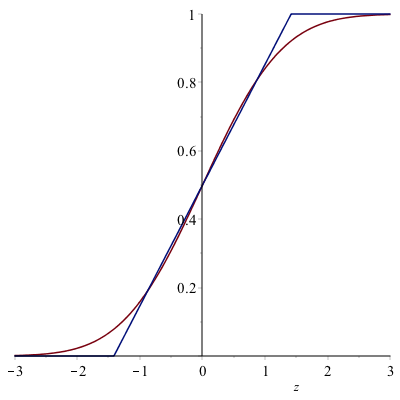
\includegraphics[scale=.5]{tables/cdf_approx.png}
\end{center}
To ballpark the effects of this approximation, I simulate a dataset with two prices and one kink point as well as simulated parameters that are close to estimated values.  Using this dataset, demand can be calculated in two ways: (1) according to the approximated function in equation (\ref{equation:generaldemand}) and (2) according to the exact demand function given by the numerical solution to the first order condition in equation (\ref{equation:firstordercondition}).  Table~\ref{table:linapproxsim} provides the parameters used for simulation as well as the simulation results.  The second and third columns provide estimates from the likelihood function in equation (\ref{equation:LLikelihood}).  The second column shows estimates when consumption is generated through the exact numerical solution to the first order conditions.  In this case, the likelihood function would be misspecified since the likelihood relies on the linear approximation.  The third column shows estimates for when consumption is generated using the linear approximation, ensuring that the likelihood function is properly specified in this case.  The estimates rely on a small sample of households in order to speed performance.  Sampling error can help explain why the estimates in column three do not exactly match the true parameters.  The last column finds small differences between estimates in columns two and three, providing some evidence that the linear approximation does not introduce substantial bias in the estimation.  Welfare differences between following  approximated versus actual versus are negligible, totaling -0.055PhP per month.

\begin{table}
\caption{Simulation Estimates for Linear Approximation}\label{table:linapproxsim}
\centering
\begin{tabular}{|lcccc|}
\hline
Parameters & Value & Est: Exact DGP  &  Est: Approx. DGP & Diff.   \\
\hline
\hline
$\sigma_{\epsilon}$  &5 &5.18 &5.01 &3.27\%  \\
$\sigma_{\eta}$  &10 &9.76 &9.92 &-1.59\%    \\
$\alpha$  &1 &0.49 &0.49 &-1.47\%    \\
$\gamma$  &[10,60] &34.72 mean &34.87 mean &-0.62\%   \\
\hline
\hline
Simulated Data &    &   &    &   \\
\hline
\hline
$P_L$ &[0,20] & & & \\
$P_H$ &[20,45] & & &  \\
Kink Point &20 & & &    \\
Households &2000 & & &    \\
Months per HH &80 & & &   \\
\hline
\end{tabular}
 \\
\footnotesize{The prices as well as the $\gamma$ terms are sampled from a uniform distribution on the given interval.  Approx. DGP stands for approximated data generating process, which generates consumption values using the linear approximation.  Exact DGP calculates consumption using the true demand function.   }
\end{table}



\section{Alternative Sharing Contracts}\label{appendix:fixedprice}

Two alternative sharing contracts include (1) alternating bill payment each month and (2) charging a fixed price to sharing households.  Alternating bill payments can be thought of as a fixed price contract where each household faces a payment of zero each month.  To model fixed price contract, consider a simple setting with two households and a linear budget constraint.  Let household $1$ pay the full bill while household $2$ pays a fixed amount $Z$ each month regardless of their consumption:.

The household optimization problems and solutions are as follows:
\begin{align*}
max_{x_1,w_1} \hspace{.2cm} & E\big[ U(x_1,w_1) \big] \\
\text{s.t.  }\hspace{.3cm} Y_1 &=   x_1  + p (W_1 + W_{2})  \\
w_1 &= \Gamma_1 - \alpha_1  p \\
max_{x_2,w_2} \hspace{.2cm} & E\big[ U(x_2,w_2) \big] \\
\text{s.t.  }\hspace{.3cm} Y_2 &=   x_1  + Z \\
w_2 &= \Gamma_2
\end{align*}
Joint consumption takes the following form:
\begin{align*}
(w_1+w_2) = (\Gamma_1 + \Gamma_2) - \alpha_1 p
\end{align*}
In the case where price sensitivities are equal between households, $\alpha_1=\alpha_2=\alpha$, joint consumption under a fixed price contract is empirically identical to joint consumption under even bill-splitting.  Therefore, assuming bill-splitting when households use fixed price contracts may bias price sensitivity estimates when these price sensitivities are very different from each other.  This bias becomes less of a concern if households alternate paying the bill because the joint estimate of $\alpha$ will capture some weighted average of $\alpha_1$ and $\alpha_2$.  Fixed price contracts may lead to a different allocation of surplus from sharing contracts depending on the size of the fixed price $Z$.  Yet, since the model assumes that households are able to split expected surplus from the sharing relationship through fixed monthly transfers in Section~\ref{section:watersourcechoice}, the type of contract likely has little effect on empirical or welfare estimates.


%%%%%%%%%%%%%%%%%%%%%%%%%%%%%%%%%%%%%%%%%%%%%%%%%%%%%%%%%%
%%%%%%%%%%%%%%%%%%%%%%%%%%%%%%%%%%%%%%%%%%%%%%%%%%%%%%%%%%  DEMAND  DEMAND  DEMAND  DEMAND  DEMAND  DEMAND  DEMAND 
%%%%%%%%%%%%%%%%%%%%%%%%%%%%%%%%%%%%%%%%%%%%%%%%%%%%%%%%%% DEMAND  DEMAND  DEMAND  DEMAND  DEMAND  DEMAND  DEMAND 
%%%%%%%%%%%%%%%%%%%%%%%%%%%%%%%%%%%%%%%%%%%%%%%%%%%%%%%%%%


\section{Descriptive for Estimation Sample}\label{appendix:descriptivesest}

\begin{table}
\caption{Descriptives for Estimation Sample}
\begin{center}
\begin{tabular}{l*{1}{cccc}}
 & & & &Standard  \\
 &Mean &Min &Max &Deviation  \\
\hline \\
\textbf{Owner Demographics} &\multicolumn{4}{c}{ }\\
\hline
Water (m3/mo.) &      27.07  &       0.00  &     100.00  &      17.67   \\
Shared 2 HHs &       0.14  &       0.00  &       1.00  &       0.34   \\
Shared Over 3 HHs &       0.09  &       0.00  &       1.00  &       0.29   \\
4 or 5 HH members &       0.41  &       0.00  &       1.00  &       0.49   \\
Over 5 HH members &       0.36  &       0.00  &       1.00  &       0.48   \\
Apartment &       0.23  &       0.00  &       1.00  &       0.42   \\
Single House &       0.59  &       0.00  &       1.00  &       0.49   \\
Low-Skill Emp. (Head of HH) &       0.17  &       0.00  &       1.00  &       0.37   \\
Two or more Empl. HH members &       0.45  &       0.00  &       1.00  &       0.50   \\
HoH Age Between 36 and 52 Yrs &       0.38  &       0.00  &       1.00  &       0.49   \\
HoH Age above 52 Yrs &       0.36  &       0.00  &       1.00  &       0.48   \\
\hline \\
\textbf{Village-Level Attributes} &\multicolumn{4}{c}{ }\\
\hline
Apt. or Single House &       0.86  &       0.00  &       1.00  &       0.08   \\
Distance Between Neighbors &       1.87  &       0.00  &      27.63  &       1.16   \\
\hline \\
\textbf{Sample Characteristics} &\multicolumn{4}{c}{ }\\
\hline
 Total Connections &\multicolumn{3}{c}{302,735 }\\
 Unconnected HHs &\multicolumn{3}{c}{286 }\\
 Number of Villages &\multicolumn{3}{c}{599 }\\
\hline
\hline
\end{tabular}
\end{center}
\end{table}



\section{Price Variation}\label{appendix:pricevariation}

\subsection{Targeting the Non-linear Tariff}

Figure~\ref{figure:consumptionhistogram} shows a histogram of monthly consumption choices across all water connections and months in the data alongside the tariff schedule (censored below 50).  Usage hovers around 20 cubic meters per month; by comparison, households in the United States use closer to 50 cubic meters per month.  Intuitively, households may be less willing to consume an additional cubic meter on the margin if the price for that unit is much higher.  The histogram provides some evidence of bunching at 10 and 20 cubic meters, although the magnitudes are quite small.  Many households are also observed to consume below 10 units where the marginal price is actually zero.  Taken together, this evidence suggests households may be unresponsive to price.

\begin{figure}
\caption{Consumption Histogram}\label{figure:consumptionhistogram}
\begin{center}
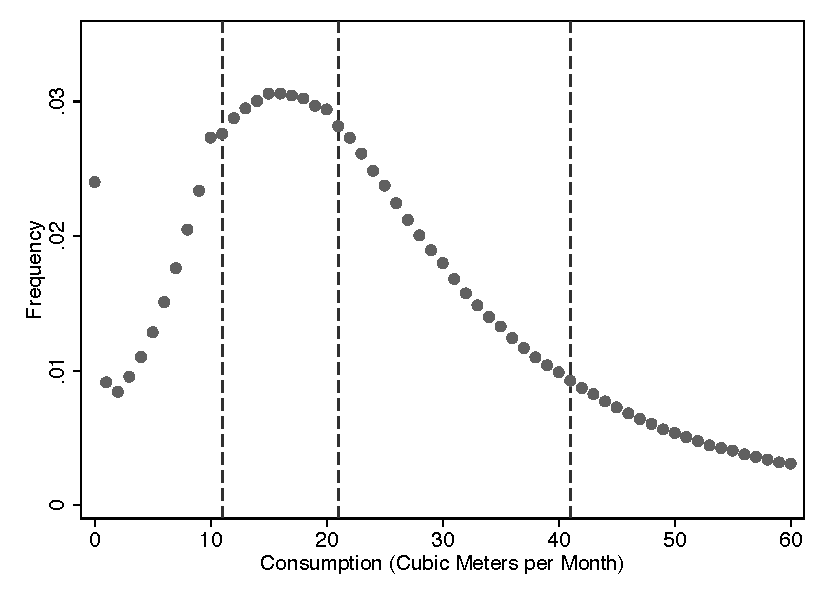
\includegraphics[scale=.7]{tables/consumption_histogram.pdf}\\
\footnotesize{Consumption values are truncated at 60 to highlight bunching at kink points.}
\end{center}
\end{figure}

\subsection{Time Series Variation in Tariffs}\label{appendix:tariffvariation}
This figure indicates time series variation in prices as a result of the government regulator raising prices incrementally to ensure production costs are covered.
\begin{figure}
\caption{Regulated Tariff Changes}\label{figure:regulatedtariffchanges}
\begin{center}
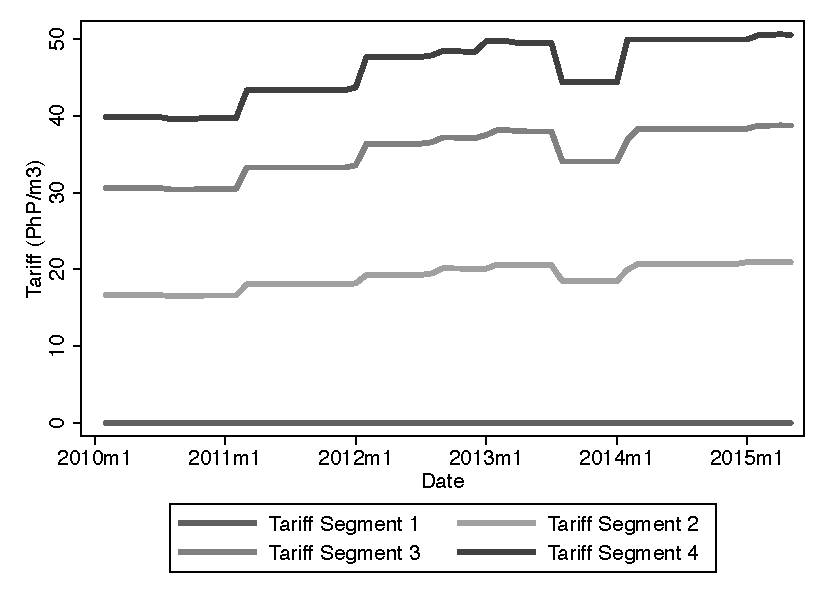
\includegraphics[scale=.7]{tables/tariff_time_series.pdf}
\end{center}
\end{figure}

\subsection{Within Connection Price Variation}\label{appendix:ratechangeelasticity}

This setting also provides quasi-experimental variation in the tariff over time at the connection-level, which serves as a useful setting to examine household demand response to price changes over time.  Previous work estimating demand for public utilities has relied on time-series variation from regulated changes in the tariff (\cite{szabo2015value,mcrae2014infrastructure}).  While the estimation strategy in this paper also includes this variation, regulated tariff changes are often relatively small, affect all households equally during the same month, and are anticipated well in advance.  Through a quirk in the regulatory agreement, the water provider is able to upgrade households that are discovered engaging small businesses to a higher tariff class called the semi-business rate.  The vast majority of these businesses are roadside stands, locally known as Sari-Sari stores.  The connection survey covers 771connections that are upgraded from residential to semi-business status used in the analysis.


Figure~\ref{figure:ressemi} compares the tariff structure between residential and semi-business rates.  The tariffs mainly deviate between 10 and 20 cubic meters where the semi-business rate is about 30\% higher.

\begin{figure}
\caption{Residential and Semi-Business Tariffs}\label{figure:ressemi}
\begin{center}
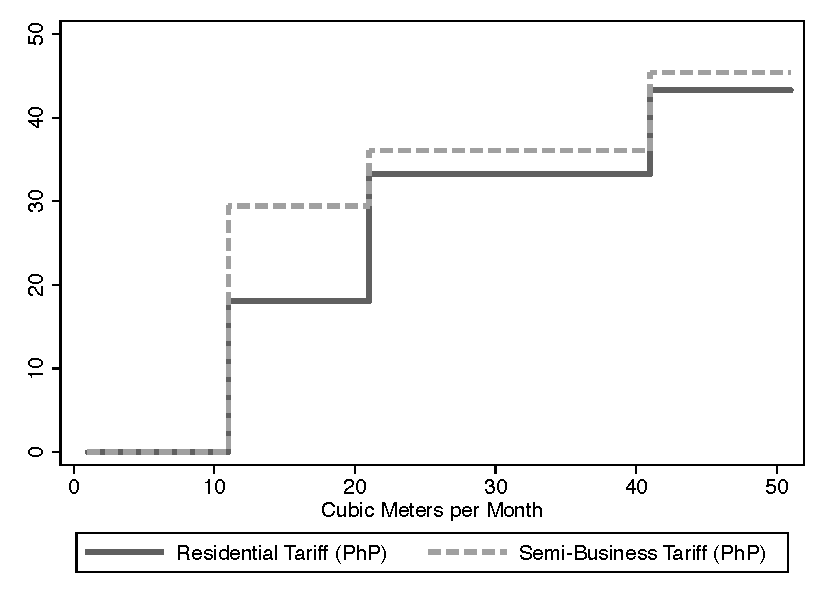
\includegraphics[scale=.65]{tables/res_semi_tariff.pdf}
\end{center}
\end{figure}

Table~\ref{table:semittests} provides summary statistics and t-tests comparing residential connections to semi-business connections, and semi-business connections to connections that are upgraded from semi-business to residential.  Semi-business connections use more water, while having smaller households sizes, greater low-skilled employment, and higher likelihoods of living in a single house.  Despite using more water, those upgraded to semi-business rates are broadly similar to the population of semi-business connections.  
%While many differences are statistically significant, the economic magnitudes of these differences are relatively small suggesting that demand responsiveness for this sub-population may be informative about the full population.

\begin{table}
\centering
\caption{Summary Statistics and Comparison of Means for Residential, Semi-Business, and Upgraded Connections}\label{table:semittests}
\resizebox{\textwidth}{!}{  
{
\def\sym#1{\ifmmode^{#1}\else\(^{#1}\)\fi}
\begin{tabular}{l*{1}{ccccc}}
\hline\hline
                    & Residential&Semi-Bus&Upgraded to &T-Test:         &T-Test:    Semi-Bus   \\
                    & Residential&Semi-Bus&Semi-Bus &Semi-Bus to Res         & to Semi-Upgrade         \\
\hline
Cons. (avg.)        &       29.42&       30.80&       35.20&       -1.37\sym{***}&       -5.78\sym{***}\\
Age HoH             &       46.26&       49.28&       46.25&       -3.01         &        0.01         \\
HH Size             &        5.15&        4.97&        5.20&        0.18         &       -0.05         \\
HH Size Empl.       &        1.58&        1.51&        1.50&        0.07\sym{*}  &        0.08\sym{*}  \\
Low Skill Emp.      &        0.16&        0.22&        0.25&       -0.06\sym{***}&       -0.09\sym{***}\\
Apartment           &        0.23&        0.14&        0.18&        0.09\sym{***}&        0.05\sym{***}\\
Single House        &        0.56&        0.68&        0.62&       -0.12\sym{***}&       -0.06\sym{***}\\
Obs.                &    47578&     5568&      771&    42010         &    46807         \\
\hline\hline
\end{tabular}
}

}\\
\footnotesize{Data are from the connection survey.}
\end{table}

The following equations estimate both event study and differences-in-differences strategies used to determine consumption response to changes in the rate class.  For connections $i$ in month $t$, these equations predict consumption as a function of individual, $\theta_i$, and time, $\delta_t$ fixed effects.  The event study in the first equation includes $\beta_r$ dummy variables for months to the rate change while the differences-in-differences approach in the second equation captures the $\beta$ effect on consumption of being after the rate-change, $Post_{i,t}$.
\begin{align*}
w_{i,t} &= \sum_{r=-12}^{12} \beta_{r} \mathbbm{1} \{t=r\}  +  \theta_{i} +\delta_t + \epsilon_{t,i} \\
w_{i,t} &= \beta Post_{i,t} +  \lambda_{1} r_{i,t} + \lambda_{2} Post_{i,t} \times r_{i,t} + \theta_{i} +\delta_t  + \epsilon_{t,i}\\
&r \text{ : month to upgrade to semi-business rate}
\end{align*}

Figure~\ref{figure:semieventstudy} plots average consumption for these connections relative to the month that they are upgraded to the semi-business tariff level.  Before the upgrade consumption trends slightly upward, before dropping immediately following the tariff increase.  A simple differences-in-differences estimate calculates a sizable price elasticity of 0.5 from this change, indicating significant demand responsiveness to time-series variation in the tariff.  This elasticity is very similar to the structural estimates in Section~\ref{section:preferenceestimation}.

\begin{figure}
\caption{Demand Response to Time Series Price Variation}\label{figure:semieventstudy}
\begin{center}
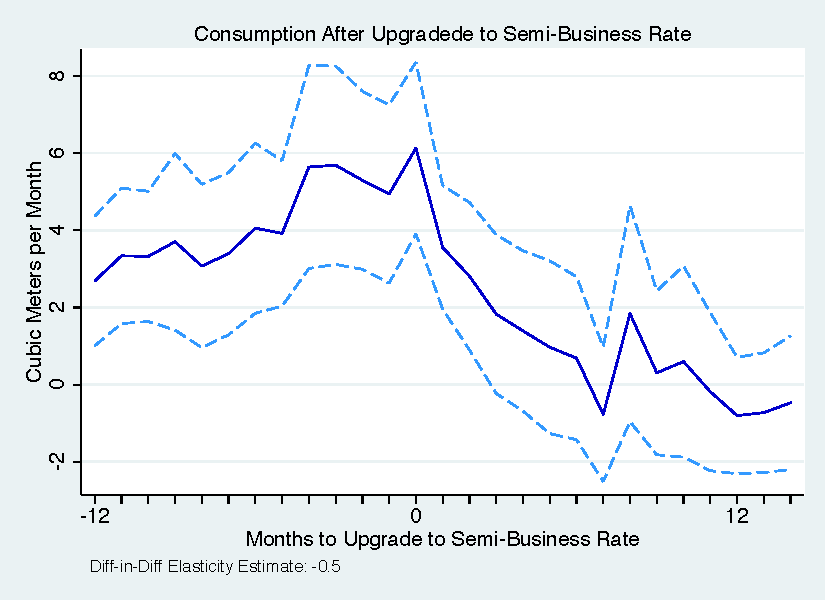
\includegraphics[scale=.7]{tables/sem_event.pdf}
\end{center}
\end{figure}







\section{Determining the Demand Function with Respect to Variance of Consumption Shocks}\label{appendix:sigmanuassumptions}

The specification of the demand function is sensitive to ex-ante assumptions on the standard deviation of the consumption shocks, $\sigma_{\epsilon}$.  To identify the appropriate demand function in this empirical setting, I maximize the likelihood function in equation (\ref{equation:LLikelihood}) over three demand specifications with different assumptions on $\sigma_{\epsilon}$ before selecting equation (\ref{equation:generaldemand}) as the primary specification.  

I first construct and estimate demand under the limiting assumption that $\sigma_{\epsilon}$ falls below the minimum threshold, $min_{\forall k}\hspace{.2cm} \{ \frac{\overline{W}_{k+1} - \overline{W}_k}{2\sqrt{2}} \} = \frac{10}{2\sqrt{2}} = 3.53$.  Under this assumption, households only consider one price at all segments and two prices near thresholds.  This assumption produces the following demand function:
\begin{align}\label{equation:demandalt1}
\begin{split}
w^{*}_C &=
\begin{cases}
D^{1}_C   & \text{ if } \hspace{1.7cm}   \frac{ \eta_C }{ V_{1,1} }  \leq \overline{\eta}^{1}_{1,L}  \\
D^{1,2}_C   & \text{ if } \hspace{.5cm} \overline{\eta}^{1}_{1,L} <    \frac{ \eta_C }{ V^{1,2} }    \leq \overline{\eta}^{2}_{1,U}  \\
D^{2}_C   & \text{ if } \hspace{.5cm} \overline{\eta}^{2}_{1,U} <    \frac{ \eta_C }{ V^{2,2} }    \leq \overline{\eta}^{2}_{2,L}  \\
D^{2,3}_C   & \text{ if } \hspace{.5cm} \overline{\eta}^{2}_{2,L} <    \frac{ \eta_C }{ V^{2,3} }    \leq \overline{\eta}^{3}_{2,U}  \\ 
D^{3}_C   & \text{ if } \hspace{.5cm} \overline{\eta}^{3}_{2,U} <    \frac{ \eta_C }{ V^{3,3} }    \leq \overline{\eta}^{3}_{3,L}  \\ 
D^{3,4}_C   & \text{ if } \hspace{.5cm} \overline{\eta}^{3}_{3,L} <    \frac{ \eta_C }{ V^{3,4} }    \leq \overline{\eta}^{4}_{3,U}  \\ 
D^{4}_C   & \text{ if } \hspace{.5cm} \overline{\eta}^{4}_{3,U} <    \frac{ \eta_C }{ V^{4,4} }   
\end{cases}\\
\text{Assuming:}\\
 \sigma_{\epsilon_C} \leq &\frac{  \overline{W}^{2} - \overline{W}^{1} }{ 2\sqrt{2} } = \frac{ 10 }{ 2 \sqrt{2} } = 3.53 
\end{split}
\end{align}
Estimates according to this demand function in the first column of Table~\ref{table:sigguess} find that the standard deviation for consumption shocks for connections serving single households through connections serving three or more households exceeds the 3.53 threshold in all cases.
\begin{table}
\centering
\caption{Alternative Demand Specification Estimates}\label{table:sigguess}
\begin{tabular}{lccc}
& $[\sigma_{\nu} < 3.53]$ & $[3.53 < \sigma_{\nu} < 7.06]$ &  $[7.06 < \sigma_{\nu} < 10.59]$ \\
Price Sensitivity : $\alpha$ &&&\\
\hline
Intercept &0.84&0.83&0.89\\
HHsize 4 to 5 &-0.02&-0.02&-0.02\\
HHsize over 5 &-0.10&-0.10&-0.10\\
Apartment &-0.04&-0.04&-0.04\\
Single House &0.05&0.05&0.05\\
Low Skill Emp. &0.02&0.02&0.02\\
Over 2 Empl. Members &0.02&0.02&0.03\\
HH Head 36 to 52 years  &0.08&0.08&0.08\\
HH Head Over 52 &0.13&0.13&0.14\\
 &&&\\
Consumption Shock : $\sigma_{\nu}$ &&&\\
\hline
Single HH &4.10&4.10&4.44\\
Two HHs &5.31&5.30&5.47\\
Three plus HHs &5.76&5.78&5.92\\
 &&&\\
Preference Shock : $\sigma_{\psi}$ &&&\\
\hline
Intercept &13.34&13.31&13.38\\
Below 1st Quintile Usage &-3.00&-2.99&-3.16\\
Over 3rd Quintile Usage &2.82&2.82&2.81\\
Two HHs &-0.48&-0.44&-0.33\\
Three HHs &1.12&1.13&1.27\\
\bottomrule
\end{tabular} \\

\end{table}
Next, I estimate the primary specification in equation (\ref{equation:generaldemand}), which holds under the hypothesis that $\sigma_{\epsilon}$ falls between $3.53$ and $\frac{\overline{W}_{2} - \overline{W}_1}{2\sqrt{2}} = \frac{20}{2\sqrt{2}} = 7.06$.  Estimates from the second column of Table~\ref{table:sigguess} fail to reject the hypothesis. 

Finally, I allow for greater variance of $\sigma_{\epsilon}$ exceeding $7.06$ and ensuring that the household responds to three prices at both interior price segments in the tariff schedule.  This specification takes the following functional form:
\begin{align}\label{equation:demandalt2}
\begin{split}
w^{*}_C &=
\begin{cases}
D^{1}_C   & \text{ if } \hspace{1.7cm}   \frac{ \eta_C }{ V_{1,1} }  \leq \overline{\eta}^{1}_{1,L}  \\
D^{1,2}_C   & \text{ if } \hspace{.5cm} \overline{\eta}^{1}_{1,L} <    \frac{ \eta_C }{ V^{1,2} }    \leq \overline{\eta}^{2}_{2,L}  \\
D^{1,2,3}_C   & \text{ if } \hspace{.5cm} \overline{\eta}^{2}_{2,L} <    \frac{ \eta_C }{ V^{1,3} }    \leq \overline{\eta}^{2}_{1,U}  \\
D^{2,3}_C   & \text{ if } \hspace{.5cm} \overline{\eta}^{2}_{1,U} <    \frac{ \eta_C }{ V^{2,3} }    \leq \overline{\eta}^{3}_{3,L}  \\ 
D^{2,3,4}_C   & \text{ if } \hspace{.5cm} \overline{\eta}^{3}_{3,L} <    \frac{ \eta_C }{ V^{2,4} }    \leq \overline{\eta}^{3}_{2,U}  \\ 
D^{3,4}_C   & \text{ if } \hspace{.5cm} \overline{\eta}^{3}_{2,U} <    \frac{ \eta_C }{ V^{3,4} }    \leq \overline{\eta}^{4}_{3,U}  \\ 
D^{4}_C   & \text{ if } \hspace{.5cm} \overline{\eta}^{4}_{3,U} <    \frac{ \eta_C }{ V^{4,4} }  
\end{cases}\\
\text{Assuming:}\\
 \sigma_{\epsilon_C} \geq &\frac{  \overline{W}^{2} - \overline{W}^{1} }{ \sqrt{2} } = \frac{ 10 }{  \sqrt{2} } = 7.06 \\
 \sigma_{\epsilon_C} \leq &\frac{  \overline{W}^{3} - \overline{W}^{2} }{ \sqrt{2} } = \frac{ 20 }{  \sqrt{2} } = 14.12
\end{split}
\end{align}
The final column in Table~\ref{table:sigguess} again rejects this hypothesis finding estimates of $\sigma_{\epsilon}$ that fall below the 7.06 threshold.  Comparing all of the parameter estimates across specifications, I find very minor differences according to the different demand functions, providing suggestive evidence that the estimation strategy is robust to ex-ante assumptions on $\sigma_{\epsilon}$.


\section{Hassle Cost: Neighbor Radius}\label{appendix:sharingneighbor}

The following equation predicts usage for neighboring households, $i$, relative to a nearby leak according to their distance rank, $DR$, relative to the leaking household with rank $1$ being closest and rank $D$ being furthest from the leaking household.  To capture any spatial changes in consumption over time, the regression also allows for differential time trends before and after the leak according to distance rank, $DR$, captured by $\lambda^{d}_{1}$ and $\lambda^{d}_{2}$:
\begin{align*}
	w_{t,i} &= \sum_{d=1}^{D} \mathbbm{1}\{DR_{i}=d\} \Big [ \beta^{d} Post_{i,t} +  \lambda^{d}_{1} r_{i,t} + \lambda^{d}_{2} Post_{i,t} \times r_{i,t} \Big ] + \theta_{i}  + \epsilon_{t,i}\\
r_{i,t} &\text{ : Months to leak} \\
DR_{i} &\text{ : Distance Rank Relative to Leaking Connection} \\
Post_{i,t} &\text{ : After leak}
\end{align*}
The coefficients of interest, $\beta^{d}$, are presented in Table~\ref{table:neighbordistance}.  I find that the closest neighbor receives the most consumption from the leaking household, closely followed by the second and fourth neighbors.  Substitution drops off quickly past the fourth neighbor, reaching statistically insignificant and economically smaller magnitudes for the fifth through eighth neighbors.  
\begin{table}
\caption{Sharing and Distance to Leaking Connection}\label{table:neighbordistance}
\centering
\begin{tabular}{lc} \hline
 & (1) \\
VARIABLES & Q (m3) \\ \hline
 &  \\
Distance Rank 1 & 0.972* \\
 & (0.504) \\
Distance Rank 2 & 0.981** \\
 & (0.444) \\
Distance Rank 3 & -0.760 \\
 & (0.479) \\
Distance Rank 4 & 0.253 \\
 & (0.512) \\
Distance Rank 5-5 & 0.216 \\
 & (0.517) \\
Constant & 22.68*** \\
 & (0.124) \\
 &  \\
Observations & 59,225 \\
R-squared & 0.678 \\
 Pre Post Trends by Rank & Yes \\ \hline
\multicolumn{2}{c}{ Robust standard errors in parentheses} \\
\multicolumn{2}{c}{ *** p$<$0.01, ** p$<$0.05, * p$<$0.1} \\
\end{tabular}

\end{table}


\section{Hassle Cost Assumptions}\label{appendix:sharingcostassumptions}

The following additional assumptions are required to ensure that this empirical setting accurately captures the model described in Section~\ref{section:hasslemodel}:
\begin{enumerate}

	\item \textit{ Connections that experience a leak are representative of the population of connections. }  This assumption is supported by minimal economic differences in means of observables between connections with leaks and without in Table~\ref{table:leakbalance} (although some differences are statistically significant).  
\begin{table}
\centering
\caption{Descriptives and Balance Test for Non-Leaking and Leaking Connections}\label{table:leakbalance}
{
\def\sym#1{\ifmmode^{#1}\else\(^{#1}\)\fi}
\begin{tabular}{l*{1}{cccc}}
\hline\hline
                    &\multicolumn{4}{c}{}                                        \\
                    &Mean No Leak&   Mean Leak&       Diff.         &  Std. Error\\
\hline
Cons. (avg.)        &       29.43&       32.42&       -2.98\sym{***}&        0.28\\
Age HoH             &       46.56&       46.36&        0.20         &        0.24\\
HH Size             &        5.14&        5.12&        0.01         &        0.03\\
HH Size Empl.       &        1.58&        1.62&       -0.04\sym{**} &        0.02\\
Low Skill Emp.      &        0.16&        0.14&        0.02\sym{***}&        0.01\\
Apartment           &        0.21&        0.23&       -0.02\sym{***}&        0.01\\
Single House        &        0.58&        0.57&        0.01         &        0.01\\
Obs.                &    56853.00&     3976.00&    52877.00         &        0.00\\
\hline\hline
\end{tabular}
}
 \\
\footnotesize{Drink is a dummy for drinking tap water.  Water flow is a dummy for low water pressure. \\ Water storage is a dummy for owning a water storage container.  Std. errors result from a T-test of differences in means.}
\end{table}

	\item  \textit{ The decision to disconnect conditional on experiencing a leak is uncorrelated with water demand. }  Table~\ref{table:leakbalancedc} provides partial support by showing few large differences in characteristics between those that disconnect and those that remain connected other than the size of leak.  This evidence suggests that the disconnection decision is driven primarily by variation in the magnitude of the leak.
\begin{table}
\centering
\caption{Balance Test for Disconnection among Leaking Connections}\label{table:leakbalancedc}
{
\def\sym#1{\ifmmode^{#1}\else\(^{#1}\)\fi}
\begin{tabular}{l*{1}{cccc}}
\hline\hline
                    &\multicolumn{4}{c}{}                                        \\
                    &  Mean No DC&     Mean DC&       Diff.         &  Std. Error\\
\hline
Cons. (avg.)        &      28.026&      30.063&      -2.037\sym{***}&       0.402\\
Leak Size           &      42.304&      59.398&     -17.094\sym{***}&       1.216\\
Age HoH             &      46.400&      46.209&       0.191         &       0.319\\
HH Size             &       5.094&       4.924&       0.170\sym{***}&       0.047\\
HH Size Empl.       &       1.538&       1.500&       0.037         &       0.024\\
Low Skill Emp.      &       0.154&       0.180&      -0.026\sym{***}&       0.008\\
Apartment           &       0.154&       0.166&      -0.012         &       0.008\\
Single House        &       0.672&       0.626&       0.046\sym{***}&       0.010\\
Obs.                &   32246.000&    2270.000&   29976.000         &       0.000\\
\hline\hline
\end{tabular}
}
 \\
\footnotesize{Drink is a dummy for drinking tap water.  Water flow is a dummy for low water pressure. \\ Water storage is a dummy for owning a water storage container. Std. errors result from a T-test of differences in means.}
\end{table}

	\item \textit{ The timing of a leak is uncorrelated with any underlying changes in demand. }  I test this assumption with a regression predicting a connection $i$'s consumption in the 30 months before the leak event controlling for a connection fixed effect, $\theta_{i}$:  
\begin{align*}
w_{t,i} &=  \sum_{r=-30}^{0} \beta_{r} \mathbbm{1} \{t=r\}  +  \theta_{i} + \epsilon_{t,i} \\
r 		 &\text{ : Month to leak}\\
\theta_i &\text{ : Connection-level fixed effect}
\end{align*}
	I include a dummy variable for each month before the leak.  Figure~\ref{figure:leakpretrend} plots demeaned monthly consumption relative to the month of the leak.  This figure shows stable a consumption pattern interrupted by a large jump at the exact time of the leak.
\begin{figure}
\centering
\caption{Pre-Trend in Leaker's Consumption}\label{figure:leakpretrend}
\begin{center}
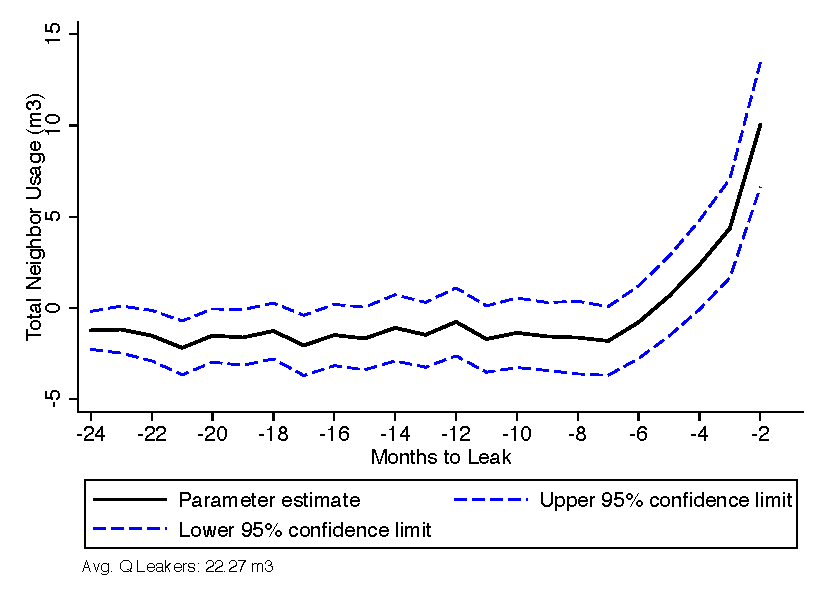
\includegraphics[scale=.7]{tables/leakers_pre_2.pdf}
\end{center}
\end{figure}

	\item \textit{ Leaks are uncorrelated with changes in neighborhood demand. }  A simple regression tests this assumption by predicting total consumption among four closest neighbors in neighborhood $N$, before and after a nearby leak, controlling for a neighborhood fixed effect, $\theta_{N}$.  I include a dummy variable for each month relative to the month that the neighbor leaks:
	\begin{align*}
	w_{N,t} &= \sum_{r=-14}^{14} \beta_{r} \mathbbm{1} \{t=r\}  +  \theta_{N} + \epsilon_{N,t} \\
	r &\text{ : Month to leak} \\
	N &\text{ : Neighborhood }
	\end{align*}
	Figure~\ref{figure:leakeventstudy} plots the results of this regression indicating average total neighborhood consumption in the months just preceding and following the date that the leakis reported.  I find a stable trend in neighbors' consumption before the leak followed by a quick leap as the leaking household starts to share with their neighbors.  This sharing behavior remains persistent for at least a year after the initial pipe leak, providing a useful window of time to estimate the hassle cost.
	\begin{figure}
	\centering
	\caption{Neighbors' Water Usage following a Leak Disconnection}\label{figure:leakeventstudy}
	\begin{center}
	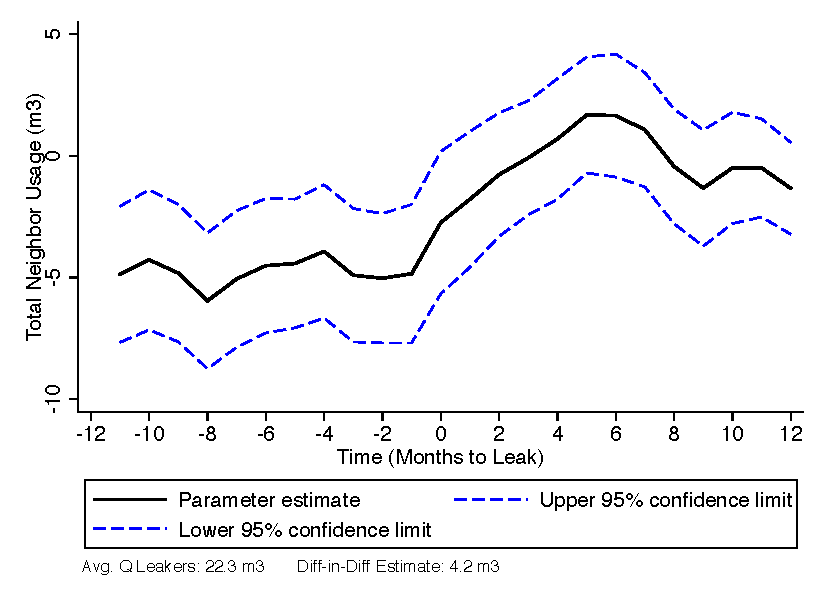
\includegraphics[scale=.7]{tables/leakers_full_2.pdf}
	\end{center}
	\end{figure}

	\item \textit{  The leaking household's choice of a sharing partner is uncorrelated with that partner's water demand.  }  This assumption holds when the $\omega$ term in equation (\ref{equation:hassleutilities}) is equal to zero.  If $\omega$ is nonzero allowing leaking households to weigh the utility from using each source in this decision, households may choose to share with low demand neighbors to enjoy lower points on the tariff in Figure~\ref{figure:tariff}.  To test this hypothesis, I predict the heterogeneous increase in neighbor's consumption following a leak according to that neighbor's water demand, which is proxied by average consumption prior to the leak.  The following regression equation tests this relationship by predicting changes in usage according to the rank of average consumption at baseline among all neighbors: 
\begin{align*}
	w_{t,i} &= \sum_{d=1}^{4} \mathbbm{1}\{Rank_{i}=d\}  \beta^{q} Post_{i,t}  + \theta_{i}  + \epsilon_{t,i}\\
r &\text{ : Month to leak} \\
Rank &\text{ : Rank of avg. usage in the neighborhood at baseline} \\
\theta_i &\text{ : Connection-level fixed effect}
\end{align*}
	One issue with this analysis is that predicting the usage response of a neighbor as a function of their previous consumption is likely to produce mean reversion bias: connections with low usage at baseline demonstrate larger increases in consumption than connections with high usage at baseline due to natural variation in preference shocks.  To test for mean reversion, I create a random treatment date using only data before the leak has occurred.  Table~\ref{table:neighborselection} presents the $\beta^{d}$ estimates of the true leak-date specification in the first column and the mean randomized leak-date estimates in the second column.  The third column takes the difference of the first and second columns, which provides a coarse method of netting out any mean reversion bias.  The first column predicts strong increases in consumption for smaller users (ranks 1 and 2) while large users (ranks 3 and 4) exhibit small and even negative demand responses.  These differential responses are only exaggerated in the second column, suggesting that mean reversion may play a large role in biasing estimates.  The third columns shows that after adjusting for mean reversion bias, the demand response of neighboring connections is roughly equal as the relative demand increases for these connections.  This finding provides suggestive evidence that households are not selecting sharing partners conditional on their neighbors' water demands.
\begin{table}
\centering
\caption{Leak Demand Response and Rank of Baseline Usage in Neighborhood}
\begin{tabular}{lccc} \hline
 & (1) & (2) & (3) \\
VARIABLES & Q (m3) & Q (m3) & Difference \\ \hline
 &  &  &  \\
Demand Rank 1 & 1.480*** & 1.334*** & 0.145 \\
 & (0.247) & (0.292) &  \\
Demand Rank 2 & 0.918** & -0.0839 & 1.002 \\
 & (0.361) & (0.398) &  \\
Demand Rank 3 & 0.157 & 1.275* & -1.117 \\
 & (0.541) & (0.663) &  \\
Demand Rank 4 & -0.122 & -0.813 & 0.691 \\
 & (1.013) & (0.929) &  \\
Demand Rank 5 & 1.769 & 4.117 & -2.348 \\
 & (1.915) & (3.283) &  \\
Constant & 22.06*** & 21.99*** &  \\
 & (0.0799) & (0.0409) &  \\
 &  &  &  \\
Observations & 59,225 & 42,108 &  \\
R-squared & 0.678 & 0.710 &  \\
Connection FE & Yes & Yes &  \\
 Simulated Leak & No & Yes &  \\ \hline
\multicolumn{4}{c}{ Robust standard errors in parentheses} \\
\multicolumn{4}{c}{ *** p$<$0.01, ** p$<$0.05, * p$<$0.1} \\
\end{tabular}
\label{table:neighborselection}
\end{table}
	\item \textit{ In response to a leak, the choice to share with a neighbor or use a vendor is uncorrelated with water demand. }  This assumption also holds when the $\omega$ term in equation (\ref{equation:hassleutilities}) is equal to zero.  If water demand were correlated with substitution across these sources, then I would expect to find that the water demand of the leaking household predicts a differential rise in usage among neighbors following the leak.  Since vended water is characterized by high prices and low fees, a simple model would predict that households with low water demand would substitute toward vendors at a higher rate and would therefore offset less consumption to neighboring households following a leak.  To test this assumption, I use average consumption for a leaking household prior to the leak as a proxy for their water demand.\footnote{Using the same test as before, I detect no evidence of mean reversion given this demand proxy.}  The following equation predicts total usage in neighborhood, $N$, before and after a household in that neighborhood experiences a leak.  The regression allows for separate impacts of a neighbor's leak, $\beta^d$ depending on that neighbor's quintile of average consumption (measured before the leak).
\begin{align*}
	w_{t,N} &= \sum_{d=1}^{5} \mathbbm{1}\{Quintile_{N}=d\}  \beta^{d} Post_{N,t}  + \theta_{N}  + \epsilon_{N,t}\\
r &\text{ : Month to leak} \\
Quintile &\text{ : Quintile of avg. usage for leaking connections at baseline} \\
\theta_N &\text{ : Neighborhood-level fixed effect}
\end{align*}
	Table~\ref{table:leakerselection} presents the results from this regression in the first column.  The size of the coefficients increase as the quintile of leaker demand increases, which is consistent with larger users at baseline using greater amounts of water from their neighbors.  To compare the relative demand response for large and small users, column three divides this coefficient estimate by the average usage for each quintile at baseline to arrive at the percentage of water consumption that is offset among neighbors after a leak occurs.  Column three finds no strong trends in the share of consumption that is offset to neighbors across water demand quintiles.  This finding provides suggestive evidence that household's are left to use whichever source is most immediately available (neighbor or vendor) following a leak.
\begin{table}
\centering
\caption{Neighborhood Usage Response and Quintile of Usage for Leaking Connection}\label{table:leakerselection}
\begin{tabular}{lccc} \hline
 & (1) & (2) & (3) \\
VARIABLES & Q (m3) & Avg. Q (m3) & Share Offset \\ \hline
 &  &  &  \\
Quintile 1 & -0.397 & 9.704 & -0.0409 \\
 & (1.612) &  &  \\
Quintile 2 & 5.290*** & 16.69 & 0.317 \\
 & (1.587) &  &  \\
Quintile 3 & 4.311** & 22.66 & 0.190 \\
 & (1.818) &  &  \\
Quintile 4 & 4.560** & 29.96 & 0.152 \\
 & (1.927) &  &  \\
Quintile 5 & 3.838** & 47.79 & 0.0803 \\
 & (1.918) &  &  \\
Constant & 65.40*** &  &  \\
 & (0.331) &  &  \\
 &  &  &  \\
Observations & 18,763 &  &  \\
R-squared & 0.788 &  &  \\
 Neighborhood FE & Yes &  &  \\ \hline
\multicolumn{4}{c}{ Robust standard errors in parentheses} \\
\multicolumn{4}{c}{ *** p$<$0.01, ** p$<$0.05, * p$<$0.1} \\
\end{tabular}

\end{table}

	\item \textit{  A leak for one household is uncorrelated with probability of a neighboring household experiencing a leak. }  While the data show little evidence that leaks  are spatially correlated, I cannot rule out unreported leaks affecting nearby households.  The presence of unobserved spatial correlation in leaks would lead this method to overestimate the hassle costs associated with sharing a connection.
\end{enumerate}


%\section{Bootstrapping Procedure for Hassle Cost}\label{appendix:hasslecostbootstrap}

%The bootstrapping procedure resamples at the level of full neighborhoods including both leaking connection and the neighboring connections, which treats each ``leak'' as its own cluster.  In a small number of bootstrapped samples ($<5\%$), the estimation procedure for this step converges to extreme outliers; this is because these samples have a relatively high share of households choosing zero monthly consumption, which are difficult values for the model to fit.  In these cases, I adjust the routine to drop zero consumption values ($<2\%$ of all values), which allows the procedure to converge to plausible parameter values.  



%\begin{align*}
%w_{i}^{pre} &= \Gamma_{i} - \alpha_{i} p \\
%w_{i}^{post} &= \Gamma_{i} - \alpha_{i} ( p + p_{h}) \\
%\frac{w_{i}^{pre} - w_{i}^{post}}{\alpha_{i}} &= p_{h}
%\end{align*}

\section{Game Tree with Three Players}\label{appendix:gametreefull}

This section maps the game tree for three players, $1$, $2$, and $3$ in Figure~\ref{figure:fullgametree}. 

%\begin{landscape}
%\setcounter{figure}{10}

\begin{figure}
\caption{Sequential Game Choosing Water Sources}\label{figure:fullgametree}
\centering
\begin{turn}{90}
\resizebox{1.1\textwidth}{!}{%
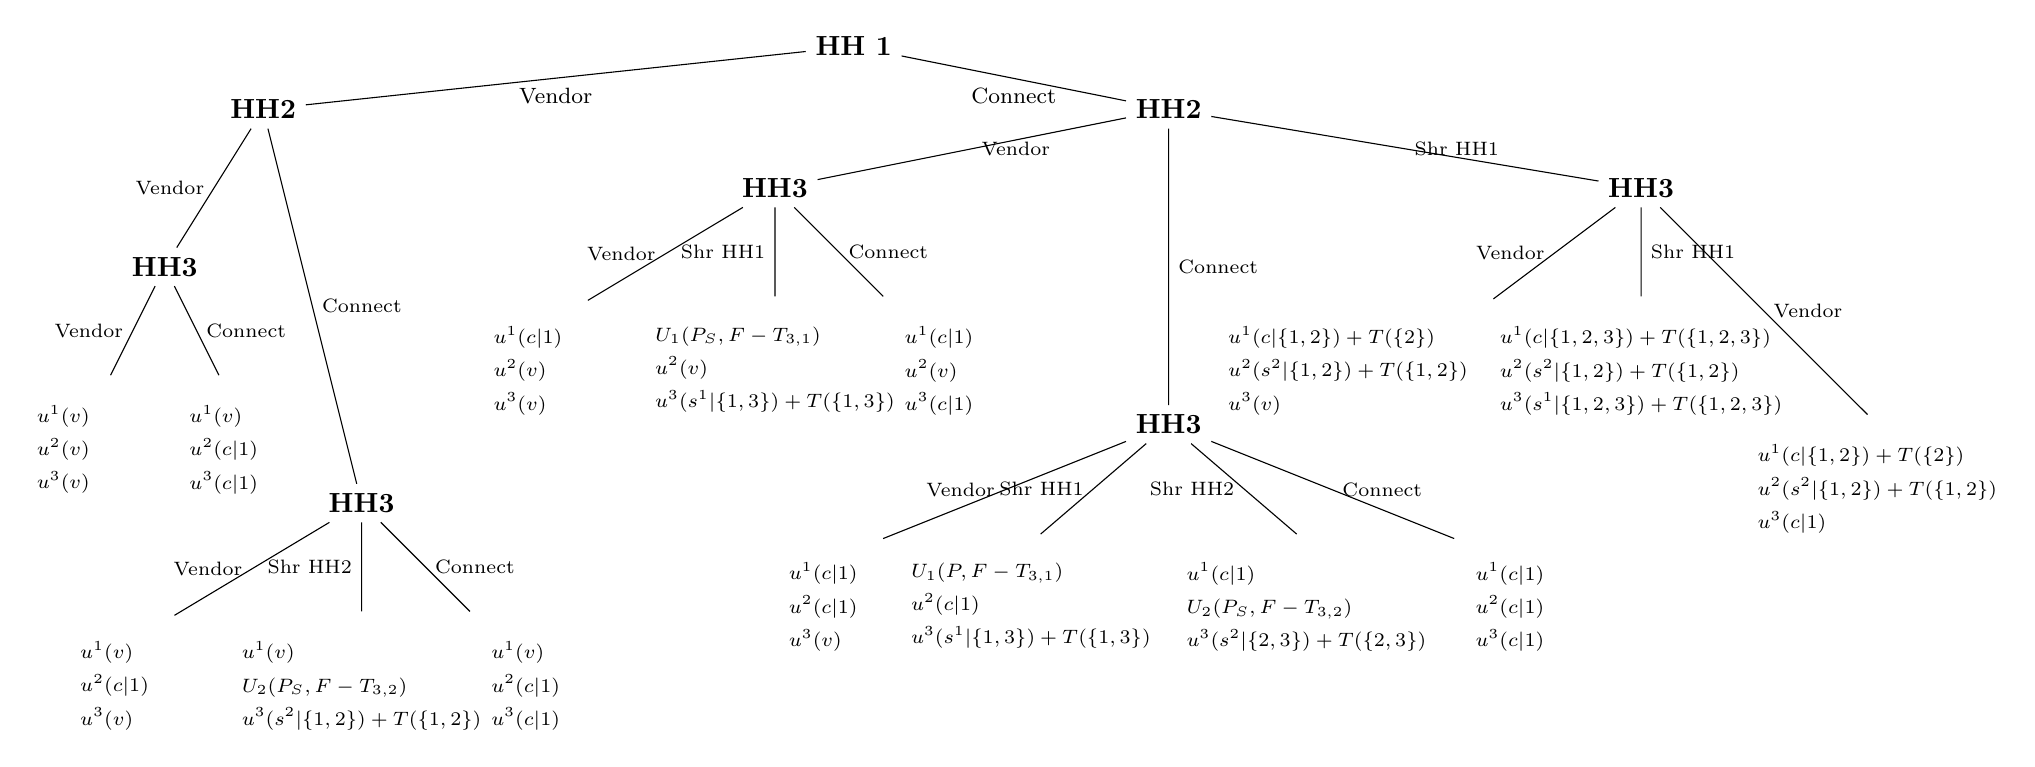
\begin{tikzpicture}
\node(0){ \textbf{HH  1}}
child[level distance=8mm,sibling distance=150mm]{node{\textbf{HH2}} %%% HERE IS NODE 1 %%%
child[level distance=20mm,sibling distance=25mm]{node{\textbf{HH3}}
child[level distance=15mm,sibling distance=15mm]{node[label={[align=left,label distance=.01cm]240: \scriptsize{$u^{1}(v)$} \\ \scriptsize{$u^{2}(v)$} \\ \scriptsize{$u^{3}(v)$}  }]{} edge from parent node[left]{\scriptsize{Vendor}}
}  
child[level distance=15mm,sibling distance=15mm]{node[label={[align=left,label distance=.01cm]270: \scriptsize{$u^{1}(v)$} \\ \scriptsize{$u^{2}(c|1)$} \\ \scriptsize{$u^{3}(c|1)$}  }]{} edge from parent node[right]{\scriptsize{Connect}}
}
edge from parent node[left]{ \scriptsize{Vendor}}
}
child[level distance=50mm,sibling distance=25mm]{node{\textbf{HH3}}
child[level distance=15mm,sibling distance=25mm]{node[label={[align=left,label distance=.01cm]240: \scriptsize{$u^{1}(v)$} \\ \scriptsize{$u^{2}(c|1)$} \\ \scriptsize{$u^{3}(v)$}  }]{} edge from parent node[left]{\scriptsize{Vendor}}
}  
child[level distance=15mm,sibling distance=25mm]{node[label={[align=left,label distance=.01cm]270: \scriptsize{$u^{1}(v)$} \\ \scriptsize{$U_{2}(P_S,F-T_{3,2})$} \\ \scriptsize{$u^{3}(s^{2}|\{ 1,2 \}) + T(\{ 1,2 \})$}  }]{} edge from parent node[left]{\scriptsize{Shr HH2}}
}
child[level distance=15mm,sibling distance=15mm]{node[label={[align=left,label distance=.01cm]280: \scriptsize{$u^{1}(v)$} \\ \scriptsize{$u^{2}(c|1)$} \\ \scriptsize{$u^{3}(c|1)$}  }]{} edge from parent node[right]{\scriptsize{Connect}}
}
edge from parent node[right]{ \scriptsize{Connect}}
}
edge from parent node[below]{ \footnotesize{Vendor} }
}
child[level distance=8mm,sibling distance=80mm]{node{\textbf{HH2}} %%% HERE IS NODE 2 %%%
child[level distance=10mm,sibling distance=50mm]{node{\textbf{HH3}}
child[level distance=15mm,sibling distance=25mm]{node[label={[align=left,label distance=.01cm]240: \scriptsize{$u^{1}(c|1)$} \\ \scriptsize{$u^{2}(v)$} \\ \scriptsize{$u^{3}(v)$}  }]{} edge from parent node[left]{\scriptsize{Vendor}}
}  
child[level distance=15mm,sibling distance=25mm]{node[label={[align=left,label distance=.01cm]270: \scriptsize{$U_{1}(P_S,F-T_{3,1})$} \\ \scriptsize{$u^{2}(v)$} \\ \scriptsize{$u^{3}(s^{1}|\{ 1,3 \}) + T(\{ 1,3 \})$}  }]{} edge from parent node[left]{\scriptsize{Shr HH1}}
}
child[level distance=15mm,sibling distance=15mm]{node[label={[align=left,label distance=.01cm]280: \scriptsize{$u^{1}(c|1)$} \\ \scriptsize{$u^{2}(v)$} \\ \scriptsize{$u^{3}(c|1)$}  }]{} edge from parent node[right]{\scriptsize{Connect}}
}
edge from parent node[right]{ \scriptsize{Vendor}}
}
child[level distance=40mm,sibling distance=50mm]{node{\textbf{HH3}}
child[level distance=15mm,sibling distance=25mm]{node[label={[align=left,label distance=.01cm]240: \scriptsize{$u^{1}(c|1)$} \\ \scriptsize{$u^{2}(c|1)$} \\ \scriptsize{$u^{3}(v)$}  }]{} edge from parent node[left]{\scriptsize{Vendor}}
}
child[level distance=15mm,sibling distance=35mm]{node[label={[align=left,label distance=.01cm]270: \scriptsize{$U_{1}(P,F-T_{3,1})$} \\ \scriptsize{$u^{2}(c|1)$} \\ \scriptsize{$u^{3}(s^{1}|\{ 1,3 \}) + T(\{ 1,3 \})$}  }]{} edge from parent node[left]{\scriptsize{Shr HH1}}
}  
child[level distance=15mm,sibling distance=35mm]{node[label={[align=left,label distance=.01cm]270: \scriptsize{$u^{1}(c|1)$} \\ \scriptsize{$U_{2}(P_S,F-T_{3,2})$} \\ \scriptsize{$u^{3}(s^{2}|\{ 2,3 \}) + T(\{ 2,3 \})$}  }]{} edge from parent node[left]{\scriptsize{Shr HH2}}
}
child[level distance=15mm,sibling distance=25mm]{node[label={[align=left,label distance=.01cm]280: \scriptsize{$u^{1}(c|1)$} \\ \scriptsize{$u^{2}(c|1)$} \\ \scriptsize{$u^{3}(c|1)$}  }]{} edge from parent node[right]{\scriptsize{Connect}}
}
edge from parent node[right]{ \scriptsize{Connect}}
}
child[level distance=10mm,sibling distance=60mm]{node{\textbf{HH3}}
child[level distance=15mm,sibling distance=20mm]{node[label={[align=left,label distance=.01cm]240: \scriptsize{$u^{1}(c|\{ 1,2 \}) + T(\{ 2 \})$} \\ \scriptsize{$u^{2}(s^{2}|\{ 1,2 \}) + T(\{ 1,2 \})$} \\ \scriptsize{$u^{3}(v)$}  }]{} edge from parent node[left]{\scriptsize{Vendor}}
}
child[level distance=15mm,sibling distance=25mm]{node[label={[align=left,label distance=.01cm]270: \scriptsize{$u^{1}(c|\{ 1,2,3 \}) + T(\{ 1,2,3 \})$} \\ \scriptsize{$u^{2}(s^{2}|\{ 1,2 \}) + T(\{ 1,2 \})$} \\ \scriptsize{$u^{3}(s^{1}|\{ 1,2,3 \}) + T(\{ 1,2,3 \})$}  }]{} edge from parent node[right]{\scriptsize{Shr HH1}}
}  
child[level distance=30mm,sibling distance=30mm]{node[label={[align=left,label distance=.01cm]270: \scriptsize{$u^{1}(c|\{ 1,2 \}) + T(\{ 2 \})$} \\ \scriptsize{$u^{2}(s^{2}|\{ 1,2 \}) + T(\{ 1,2 \})$} \\ \scriptsize{$u^{3}(c|1)$}  }]{} edge from parent node[right]{\scriptsize{Vendor}}
}
edge from parent node[right]{ \scriptsize{Shr HH1}}
}
edge from parent node[below]{ \footnotesize{Connect} }
}
;
%\node at($(0-1)!.7!(0-2)$){ \textbf{HH 2} };
%\node at($(2-1)!.5!(2-2)$){ \textbf{HH 3} };
\end{tikzpicture}
}
\end{turn}
%\begin{itemize}
%\item $p_v$: Vendor Price
%\item $F_v$: Vendor Fee/Disutility
%\item $T_{i,j}$: Transfer from household $i$ to household $j$
%\item $P, P_S$: Tariff schedules for single and joint users
%\item $p_{h}$: Hassle Cost
%\end{itemize}
\end{figure}

%\end{landscape}

\section{Test for Incidental Parameter Bias}\label{appendix:incidentalparametertest}

The estimation strategy relies heavily on connection-specific fixed preference terms estimated in the Section~\ref{section:preferenceestimation} to recover parameters in Section~\ref{section:hasslecostestimation} and Section~\ref{section:fixedcostestimation}.  Since the data contain a limited number of months of consumption for each connection (averaging around 77 months), noise in the estimation of these preference terms may produce bias in latter estimates.  I test for this type of bias by simulating data given true parameters close to the estimates and reestimating the model on this simulated data.  Table~\ref{table:incidentalparameters} provides results for this test.  

The first column presents the true assumed parameter values, the second column provides the estimations results for the simulated data using the full sample, and the third column includes estimates for a subsample of the data where I have dropped half of the observations for each connection.  Examining the second column and percent deviations in the third column, I find that the incidental parameters do not seem to lead to a large degree of bias in any of the coefficients with the maximum occurring for the variance estimate for the vendor price.  Dropping half of the time periods, the fourth and fifth columns indicate that the hassle cost and connection fee parameters would be the most sensitive to any possible bias from incidental parameters.

\begin{table}

\centering
\caption{Simulation Test for Incidental Parameter Bias}\label{table:incidentalparameters}
\begin{tabular}{lccccc}

Parameter & True Value & Est: Full T & (\% Diff)  & Est: 50\% T & (\% Diff) \\
\hline
\hline
$\sigma_{\epsilon}$&5.00&5.03&0.01&5.01&0.00\\
$\sigma_{\eta}$&12.00&11.91&-0.01&11.79&-0.02\\
$\alpha$&0.50&0.51&0.02&0.51&0.03\\
$\gamma$ (avg.)&34.32&34.60&0.01&33.98&-0.01\\
$p_h$&15.00&14.17&-0.06&11.74&-0.22\\
$F$&400.00&393.72&-0.02&378.30&-0.05\\
$F_v$&100.00&99.87&-0.00&98.70&-0.01\\
$p_v$&40.00&41.00&0.02&40.48&0.01\\
$\sigma_v$&5.00&5.69&0.14&5.88&0.18\\
\hline
\end{tabular}
\\
\footnotesize{T refers to months observed for each connections.  The first sample includes half of the time periods per connection (around 35 months), while the second sample includes all months.  Both samples include 5,000 accounts.}
\end{table}


\end{appendices}


{
\small
\nocite{*}
\bibliographystyle{abbrvnat}
\setcitestyle{authoryear,open={((},close={))}}
\bibliography{library}
}



%\begin{center}
%  \input{mean_diff_leak1}
%\end{center}

%\begin{center}
%    \input{mean_diff_DC1}
%\end{center}



% \begin{table}[]
% \centering
% \caption{Source Choices}
% \label{my-label}
% \begin{tabular}{|l|c|c|c|}
% \hline
%                 & Fixed Price                  & Marginal Price                 & Tariff Kink Points      \\ \hline
% Individual (I)  & $F$                          & $P_k$                         & $\overline{w}_{k}$                         \\ \hline
% Shared   (S)    & $\frac{F}{2}$                & $P_k + P_{h}$                 & $\frac{\overline{w}_{k}}{2}$                            \\ \hline
% Vendor   (V)    & $0$                          & $P_{v}$                        & $0$                          \\ \hline
% \end{tabular}
% \end{table}
%\bibliography{lib}


\end{document}  